%% This is file `elsarticle-template-1-num.tex',
%%
%% Copyright 2009 Elsevier Ltd
%%
%% This file is part of the 'Elsarticle Bundle'.
%% ---------------------------------------------
%%
%% It may be distributed under the conditions of the LaTeX Project Public
%% License, either version 1.2 of this license or (at your option) any
%% later version.  The latest version of this license is in
%%    http://www.latex-project.org/lppl.txt
%% and version 1.2 or later is part of all distributions of LaTeX
%% version 1999/12/01 or later.
%%
%% The list of all files belonging to the 'Elsarticle Bundle' is
%% given in the file `manifest.txt'.
%%
%% Template article for Elsevier's document class `elsarticle'
%% with numbered style bibliographic references
%%
%% $Id: elsarticle-template-1-num.tex 149 2009-10-08 05:01:15Z rishi $
%% $URL: http://lenova.river-valley.com/svn/elsbst/trunk/elsarticle-template-1-num.tex $
%%
\documentclass[preprint,12pt]{elsarticle}

\usepackage{algorithm}
\usepackage{algorithmic}
\usepackage{graphicx,subfigure}
\usepackage{multirow,color}
\usepackage{amsmath}
\usepackage{url,hyperref}

%% Use the option review to obtain double line spacing
%% \documentclass[preprint,review,12pt]{elsarticle}

%% Use the options 1p,twocolumn; 3p; 3p,twocolumn; 5p; or 5p,twocolumn
%% for a journal layout:
%% \documentclass[final,1p,times]{elsarticle}
%% \documentclass[final,1p,times,twocolumn]{elsarticle}
%% \documentclass[final,3p,times]{elsarticle}
%% \documentclass[final,3p,times,twocolumn]{elsarticle}
%% \documentclass[final,5p,times]{elsarticle}
%% \documentclass[final,5p,times,twocolumn]{elsarticle}

%% if you use PostScript figures in your article
%% use the graphics package for simple commands
%% \usepackage{graphics}
%% or use the graphicx package for more complicated commands
%% \usepackage{graphicx}
%% or use the epsfig package if you prefer to use the old commands
%% \usepackage{epsfig}

%% The amssymb package provides various useful mathematical symbols
\usepackage{amssymb}
%% The amsthm package provides extended theorem environments
%% \usepackage{amsthm}

%% The lineno packages adds line numbers. Start line numbering with
%% \begin{linenumbers}, end it with \end{linenumbers}. Or switch it on
%% for the whole article with \linenumbers after \end{frontmatter}.
%% \usepackage{lineno}

%% natbib.sty is loaded by default. However, natbib options can be
%% provided with \biboptions{...} command. Following options are
%% valid:

%%   round  -  round parentheses are used (default)
%%   square -  square brackets are used   [option]
%%   curly  -  curly braces are used      {option}
%%   angle  -  angle brackets are used    <option>
%%   semicolon  -  multiple citations separated by semi-colon
%%   colon  - same as semicolon, an earlier confusion
%%   comma  -  separated by comma
%%   numbers-  selects numerical citations
%%   super  -  numerical citations as superscripts
%%   sort   -  sorts multiple citations according to order in ref. list
%%   sort&compress   -  like sort, but also compresses numerical citations
%%   compress - compresses without sorting
%%
%% \biboptions{comma,round}

% \biboptions{}


\journal{Computer Networks}

\begin{document}

\begin{frontmatter}

%% Title, authors and addresses

%% use the tnoteref command within \title for footnotes;
%% use the tnotetext command for the associated footnote;
%% use the fnref command within \author or \address for footnotes;
%% use the fntext command for the associated footnote;
%% use the corref command within \author for corresponding author footnotes;
%% use the cortext command for the associated footnote;
%% use the ead command for the email address,
%% and the form \ead[url] for the home page:
%%
%% \title{Title\tnoteref{label1}}
%% \tnotetext[label1]{}
%% \author{Name\corref{cor1}\fnref{label2}}
%% \ead{email address}
%% \ead[url]{home page}
%% \fntext[label2]{}
%% \cortext[cor1]{}
%% \address{Address\fnref{label3}}
%% \fntext[label3]{}

\title{Early Flow Discard for Packet Scheduling over Wired and Wireless links}

%% use optional labels to link authors explicitly to addresses:
%% \author[label1,label2]{<author name>}
%% \address[label1]{<address>}
%% \address[label2]{<address>}

\author[*]{Jinbang Chen}
\author[**]{Martin Heusse}
\author[***]{Guillaume Urvoy-Keller}
\address[*]{East China Normal University, China\footnote{This study was carried out while the author was at Eurecom, 450 Route des Chappes, 06410 Biot France}}
\address[**]{Laboratoire LIG CNRS UMR 5217, Grenoble, France}
\address[***]{Univ. Nice Sophia Antipolis, CNRS, I3S, UMR 7271, 06900 Sophia Antipolis}
\begin{abstract}
%% Text of abstract

\end{abstract}

\begin{keyword}
Priority scheduling \sep TCP \sep Performance \sep Flows \sep QoS \sep 802.11
%% keywords here, in the form: keyword \sep keyword

%% MSC codes here, in the form: \MSC code \sep code
%% or \MSC[2008] code \sep code (2000 is the default)

\end{keyword}

\end{frontmatter}

%%
%% Start line numbering here if you want
%%
% \linenumbers

%% main text
\section{Introduction}
\label{sec:intro}


To improve the Quality of Experience of end users, two general approaches exist. The first one involves the deployment of end-to-end mechanisms like IntServ and DiffServ.  This appears out of reach at the moment as it requires ISPs to cooperate with one another with an unclear business model if ISPs remain simple bit carrier unable to attract advertising revenues. In addition, it is against the Internet philosophy that consists in pushing the intelligence at the edge, \textit{i.e.}, leaving applications decide how they utilize a best effort network. The second approach is fully decentralized and offers a toolbox of traffic management mechanisms that ISP can deploy in their network equipments, mostly switches and routers.  These mechanisms include  scheduling and buffer management policies like \textit{e.g.}, FIFO and Fair Queuing (FQ) which are popular scheduling policies; while droptail, RED \cite{Floyd93} or, more recently, CoDel \cite{Jacobson12} are examples of buffer management policies. As highlighted by Sivaraman \textit{et al.} \cite{sivaraman2013no}, the exact combination of policies to use depends on the set of applications, their QoS requirements as well as on the underlying access network, \textit{e.g.}, wired or wireless, cellular networks. There is no one size fits all solution. Still, a consensus exists concerning the (conflicting) objectives to reach: a highly utilized network with minimally utilized buffers. Indeed, as buffers aim at acting as shock absorbers, they lead to delay increase if they are continuously utilized \cite{Jacobson12}. Failure to meet these requirements can lead to the so-called bufferbloat phenomenon \cite{Gettys12}, as observed in wired and mobile networks \cite{BufferBloat_IMC_2012}.

RED and CoDel are two solutions to keep the buffers' occupancy low. 
The two key challenges faced by these active queue management (AQM) mechanisms is to assess the queue utilization and decide which flow to penalize in case the queue utilization is deemed too high. Penalizing a short flow might be detrimental to the end users as those flows are often generated by interactive applications (Web browsing, email, DNS queries, tweets, chats, \ldots). Penalizing a high rate flow might be a good strategy if this flow requires a low delay, while it can be under optimal in the case of a download to a mobile device, see \cite{sivaraman2013no}. An approach to solve this dilemma (which flow to penalize) is to  use a size-based scheduler, \textit{e.g.}, SRPT \cite{kleinrock_76_queueing},  LAS/LARS \cite{Rai02size-basedscheduling,Martin10Lars} or Run2C \cite{Avrachenkov04Run2c}. A size-based scheduler is flow aware as it takes the flow size or flow rate into account in its scheduling (and also buffer management) decision. When applied to the case of Internet traffic that consists of a mix of short and large flows, the idea behind size-based scheduling is to give priority to short flows and long flows in their early stage (which we call young flows hereafter) so as to favor interactive applications and, more generally, TCP flows in their infancy. It is indeed known that TCP is more sensitive to loss and delays in its slow start phase than during the later congestion avoidance phase. While size-based scheduling does not try to limit the queue size, it alleviates the bufferbloat  phenomenon by granting short/young flows access to the head of the queue, which in general results in a response time almost independent of the physical queue size and actual load condition. 

There is however a price to pay to use size-based scheduling, which is the bookkeeping cost of tracking each and every active flows at the switch/router. %The overhead for flow state keeping have arisen more and more concern in the research community \cite{chen2011efd, DivakaranAP11,Divakaran2012networks} mainly due to the scalability consideration. 
Indeed, a flow table is required that needs to be updated for every arriving packet \footnote{The authors of \cite{Avrachenkov04Run2c} proposed an elegant solution to work around this issue by encoding the flow size into the TCP sequence number. However, such a solution requires modifications of (and trust in) every end hosts}. %Given that the action involves table lookup, memory access and update, it will require the ability of fast access as well as high processing power. 
In addition, the number of flows in progress can grow to a large value under high load. 
Recent advances in the SDN (Software Defined Routers) demonstrate that bookkeeping of flows in commercial routers is possible. However, SDN aims at exposing the control plane and not the data plane of a switch, hence some recent efforts to extend SDN to enable the implementation of scheduling/buffer management policies, see \textit{e.g.}, \cite{sivaraman2013no}.
%Besides, some policies feature other drawbacks. LAS may lead to severe starvation to long flows, which is known as ``lock-out'' phenomenon. Moreover, LAS and Run2C scheduling policies consider a single dimension of a flow, namely its accumulated sizes. Still, persistent low rate transfers often convey key traffic, \textit{e.g.}  voice over IP conversations. As a result, it seems natural to account both for the rate and the accumulated amount of bytes of each flow. 

In this work, we explore a radical approach to the scalability issue of size-based scheduler by limiting the memory of the scheduler to the packets in the buffer. Our scheduler, that we call  EFD (Early Flow Discard) features the following properties: (i) Low response time to small and young flows, irrespectively of queue size and load; (ii) Low bookkeeping cost, \textit{\textit{i.e.}}, the number of flows tracked at any given time instant remains consistently low; (iii) Differentiation of flows based on volumes but also on rate; (iv) Avoidance of lock-outs. The two latter properties are known deficiencies of formely proposed size-based scheduler. The former occurs if a low rate flow, \textit{e.g.}, a VoIP transfer, runs for a long time and appears fat to the scheduler that simply accumulates transferred volume of flows like LAS or Run2C. The latter refers to the race condition that can occur if a long flow starts while another long flow has sent a lot of bytes, which can lead to a starvation of the older one. LARS, which accounts jointly for volumes and rates is able to work around this problem. We demonstrate that EFD behave similarly to LARS with a memory footprint orders of magnitude lower.% to its limited memory.

%EFD manages the physical queue of an interface (at the IP level) as a set of two virtual queues corresponding to two levels of priority: the high priority queue first and the low priority queue at the tail of the buffer. Formally, EFD belongs to the family of Multi-Level Processor Sharing policies (see Section \ref{sec:related}) and is effectively a PS+PS scheduling policy. The key difference between EFD and other MLPS scheduling disciplines is the way flow states are handled. In EFD, we keep an active entry only for flows that have at least one packet present in the queue. A flow entry is deleted from the flow table upon the departure of last packet of this flow currently residing in the queue. This simple approach allows to fulfill the entire list of objectives listed above. Specifically, in EFD the active flow table size is bounded to a low value. Also, although EFD  has a limited memory footprint, it can discriminate against bursty and high rate flows. EFD is not limited to a scheduling policy but also incorporates a buffer management policy, where the packet with smallest priority gets discarded when the queue is full, as opposed to drop tail which blindly discards packets upon arrival. This mechanism is similar to the one used in previous works \cite{Rai04size-basedscheduling,DivakaranCAP10}. We first assess the performance of EFD in wired networks.

The remaining of this paper is organized as follows. Section \ref{sec:related} reviews the previous work on mitigating the biases against small flows. The detailed description of EFD discipline and its adaptation to WLANs are given in Section \ref{sec:efd_alg}. We then present the performance evaluation of EFD in wired network and in 802.11 wireless network respectively in Section \ref{sec:perf_wired} and Section \ref{sec:perf_wlan}. In Section \ref{sec:analysis_efd}, we present an analytical model of EFD, which helps to explain the performance discrepancy observed among EFD's flavors. 

%\textcolor{red}{Old intro starts here:}

%As the Internet evolves over the years, many of the new applications emerge with varying QoS requirements such as low response time, guaranteed loss rate and so on. The legacy FIFO/drop-tail scheme deployed in today's routers/switches, is believed to favor long transfers at flow level, which in reverse highly restricts the transmission of short transfers - one sees the need of improvement since short flows are in general related to interactive applications - such examples include Web browsing, Email checking, DNS queries, and more recently tweets, chats, \textit{etc.} - for which users expect very short response times, while long flows represent background traffic, usually the downloads involving bulk data transfers. 

%The resource sharing issue in computer networks has been studied for decades and many scheduling algorithms were first developped in the context of job scheduling in operating systems. Packet scheduling has been re-activated in the research community in the last decade due to the studies of job size distributions in a variety of computing contexts including Web file sizes \cite{Crovella1997,Barford1998}, FTP file transfers \cite{Rai02fb,Guo2002Scheduling}, UNIX job sizes, and more. In all these cases, job size distribution has been shown to exhibit heavy tails, and be well-modeled by a Pareto distribution, or some other distributions with a power-law tail. This new finding calls for re-evaluation of scheduling policies with heavy-tailed workload in the Internet \cite{WillingerTSW97}, in particular for size-based scheduling policies. 

%The strong heavy-tailed bahavior observed for Internet flow size distribution refers to the fact that a small percentage of very long flows contribute to a large percentage of the Internet traffic volumes, known as mice-elephants rule \cite{guo01icnp} or 90-10 rule \cite{Collange08jucs}. Consequently, many size-based solutions to the biases against small flows in current Internet architecture have been proposed. The key idea is to favor short flows at the expense of long ones. Such a strategy pays off as long as long flows are not completely starved and this generally holds without further intervention for Internet traffic where short flows represent a small portion of the load and thus cannot monopolize the bandwidth. 

%To enhance the performance -- most often, the response time -- of short TCP flows (\textit{i.e.} the interactivity) over a best-effort network, most effort of designing a size-based scheduler generally relies on every attempt on the two main factors dominating the latency performance:

%\begin{itemize}
%\item the end-to-end transfer time. Research has shown that the queueing time makes up a significant fraction of the end-to-end transfer time, in particular at high load. It is therefore helpful to improve the response time of short flows if the queueing delay of their packets can be reduced;
%\item the possible packet losses, particularly at the beginning of a connection. The losses of the first few packets in the early infancy of a connection (\textit{i.e.} in the slow start stage) are usually recovered by the retransmisson timeout (RTO) mechanism as the TCP slow start limits the number of packets needed to triger fast retransmit (FR). Moreover, the initial RTO is set to a large value (a conventional value of 3 seconds is recommended in RFC 2988) , which eventually worsens the latency performance. 
%\end{itemize}
%
%Basically, the reduction of queueing time in the buffer can be achieved by preferential scheduling - in which packets from some types of flows are scheduled prior to packets from other flows, \textit{i.e.} prioritization in time, whereas the packet losses might be improved with the help of proper buffer management policies, \textit{i.e.} prioritization in space. Most of solutions proposed give priority to small flows over long flows in either or both of the two dimensions: space and time, thereby improving the response time of small flows. They have evolved from SRPT \cite{kleinrock_76_queueing} to LAS/LARS \cite{Rai02size-basedscheduling,Martin10Lars} and MLPS scheduling policies like Run2C \cite{Avrachenkov04Run2c}. The different size-based schedulers need to identify flows and distinguish between small and large flows. Some of them base on the ongoing size (or remaining size) of the flows such as SRPT and LAS/LARS, while Run2C applys a strict threshold with empirical values. Other works use a legacy FIFO as the scheduling policy, along with an Active Queue Management(AQM) strategy which gives preferential treatment to packets of small flows in space. 
%However, a common drawback shared by most of such works dealing with giving preferential treatment based on the size is observed, that is the router/switch which implements such scheduling policies need to keep track of all flows to assist on scheduling each arriving packet. The overhead for flow state keeping have arisen more and more concern in the research community \cite{chen2011efd, DivakaranAP11,Divakaran2012networks} mainly due to the scalability consideration. Remind that keeping track of sizes of all flows is changing as it requires flow table update for every arriving packet. Given that the action involves table lookup, memory access and update, it will require the ability of fast access as well as high processing power. In addition, the number of flows in progress can grow to a large value in high load. Besides, some policies feature other drawbacks. LAS may lead to severe starvation to long flows, which is known as ``lock-out'' phenomenon. Moreover, LAS and Run2C scheduling policies consider a single dimension of a flow, namely its accumulated sizes. Still, persistent low rate transfers often convey key traffic, \textit{e.g.}  voice over IP conversations. As a result, it seems natural to account both for the rate and the accumulated amount of bytes of each flow. 

%We present a new scheduling policy, EFD (Early Flow Discard) that aims at fulfilling the following objectives: (i) Low response time to small flows; (ii) Low bookkeeping cost, \textit{\textit{i.e.}}, the number of flows tracked at any given time instant remains consistently low; (iii) Differentiating flows based on volumes but also based on rate; (iv) Avoiding lock-outs.

%EFD manages the physical queue of an interface (at the IP level) as a set of two virtual queues corresponding to two levels of priority: the high priority queue first and the low priority queue at the tail of the buffer. Formally, EFD belongs to the family of Multi-Level Processor Sharing policies (see Section \ref{sec:related}) and is effectively a PS+PS scheduling policy. The key difference between EFD and other MLPS scheduling disciplines is the way flow states are handled. In EFD, we keep an active entry only for flows that have at least one packet present in the queue. A flow entry is deleted from the flow table upon the departure of last packet of this flow currently residing in the queue. This simple approach allows to fulfill the entire list of objectives listed above. Specifically, in EFD the active flow table size is bounded to a low value. Also, although EFD  has a limited memory footprint, it can discriminate against bursty and high rate flows. EFD is not limited to a scheduling policy but also incorporates a buffer management policy, where the packet with smallest priority gets discarded when the queue is full, as opposed to drop tail which blindly discards packets upon arrival. This mechanism is similar to the one used in previous works \cite{Rai04size-basedscheduling,DivakaranCAP10}. We first assess the performance of EFD in wired networks.

%\subsection{Scheduling policies for bi-directional traffic control over half-duplex links}
%When taking into account both directions of flows, LAS can be easily extended, leading to the definition of LASACK for 802.11 WLANs \cite{Keller2008Improving}. In an 802.11 network setting, two key properties lead to the TCP performance problem: (i)the protocol is half-duplex, meaning that uploads and downloads share the wireless medium and (ii) the access point (AP) is not granted a high enough priority to access the medium under the Distributed Coordination Function (DCF) at the MAC layer as compared to the other stations in the cell \cite{Pilosof03understandingtcp}, meaning that its queue, which is typically 30 to 100 packets, tends to build up. The main idea behind LASACK, and later LARS \cite{heusse2011least} when deployed in 802.11 WLANs for handling bi-directional traffic, is to look up the acknowledgment number in the TCP header and add its progress since the previous segment to the virtual service size of the corresponding connections. So that the virtual service size of a TCP connection is the total amount of data traffic that has been transferred by the flow so far. This is the key to offer similar bandwidth sharing to uploads and downloads, and turn out to be efficient in an 802.11 WLAN scenario \cite{Keller2008Improving, heusse2011least}. 
%
%Another objective of this paper is to test EFD's applicability to WLAN infrastructure networks. We propose two adaptations of EFD in WLAN networks, EFDACK and PEFD,  that aim at mitigating the TCP unfairness problem. EFDACK keeps  track of the amount of bytes sent by each flow in both the upload and download directions, which requires reading TCP segments (the acknowledgment number field) within IP packets. This is the same idea as the one of LASACK \cite{Keller2008Improving}. In contrast, PEFD keeps track of the number of packets and does not distinghuish between uploads and downloads. 
%
%Overall, in this paper, we have evaluated the perfromance of EFD in wired network and wireless network (802.11 WLANs configuration) by extensive simulations, and compared it with a wide range of scheduling policies. Besides, we have also discussed the flavors of EFD - two disciplines (FIFO and LAS) are respectively deployed in two priority queues, resulting at four different combinations: FIFO+FIFO, FIFO+LAS, LAS+FIFO and LAS+LAS. Finally, we have slightly hit the issue towards the analitic model for EFD. The remaining of this paper is organized as follows. Section \ref{sec:related} discusses the previous work on mitigating the biases againt small flows. The detail description of EFD discipline and its adaptation to half-duplex links are given in Section \ref{sec:efd_alg}. We then present the performance evaluation of EFD in wired network and in 802.11 wireless network respectively in Section \ref{sec:perf_wired} and Section \ref{sec:perf_wlan}. In Section \ref{sec:analysis_efd}, we have proposed a model for shifting from subflows to flows, which helps to explain the performance discrepancy observed among EFD's flavors. And finally, Section \ref{sec:conclu} concludes the paper.  


\section{Related works}
\label{sec:related}
Size-based scheduling has received a lot of attention from the research community with applications to Web servers \cite{SRPT_Web2006}, Internet traffic \cite{Avrachenkov04Run2c,Rai2004Performance,Keller2008Improving} or 3G networks \cite{Aalto2007Impact,Lassila2008Combining}. Classically, size-based scheduling policies are divided into blind and non-blind scheduling policies. A blind size-based scheduling policy is not aware of the job\footnote{Job is a generic entity in queueing theory. In the context of this work, a job corresponds to a flow.} size while a non-blind is. A typical example of non blind policy is the Shortest Remaining Processing Time (SRPT), which is known to be optimal \cite{Schrage1968SRPT}, in the sense that it minimizes the average response time of transfers. To achieve this property, SRPT relies on a simple strategy: always service the client that is the closest to completion. SRPT scheduling has been proposed for web servers \cite{Chen03cnetworks,Harchol2003}. Although appealing, SRPT is impractical as it requires prior knowledge of flow sizes - which is not achievable for most networking elements (router, access point, \textit{etc}.). Therefore, more attention is given to blind size-based scheduling policies, \textit{i.e.} the schedulers that are not aware of the flow size.

%We restrict ourselves to a seminal subset of methods proposed in the literature.
 Least Attained Service (LAS) policy \cite{Rai02size-basedscheduling}, gives priority to the flow that has received the least amount of service so far. In case that there are multiple flows with least amount of service received, all of them share the bandwidth equally in a processor sharing (PS) manner. LAS is known to be optimal if the flow size distribution has a decreasing hazard rate (DHR) \cite{Nuyens2008FB} as it becomes, in this context, a special case of the optimal Gittins policy \cite{Gittins89}.  It is well-established that LAS is able to decrease the response time and loss rate of short flows compared to a FIFO scheduler with drop-tail buffer management policy, at the expense of negligible increase in response time for long flows \cite{Rai02size-basedscheduling,Rai04size-basedscheduling,Rai04performancemodels}. As an extension of LAS, Least Attained Recent Service (LARS) \cite{Martin10Lars} applies a temporal decay to the volume of data associated with each flow. With this strategy, LARS bounds the impact of a new flow on ongoing ones and accounts not only for the volumes, but also the rate of flows. However, the implementation of LAS and LARS require to keep track of each and every ongoing flow so as to decide which packet/flow to serve next, where the processing is complex and overhead-consuming. In addition, LAS features some other drawbacks, such as starvation of long flows.% and flow discrimination based on volume (\textit{i.e.}the accumulated amount of bytes of each flow) only. 

Some representatives of the family of Multi-Level Processor Sharing \linebreak[4] (MLPS) scheduling policies \cite{kleinrock_76_queueing} have also been proposed to favor short flows. An MLPS policy consists of several levels corresponding to different amounts of attained service of jobs, with possibly a different scheduling policy at each level. As a PS+PS model, Run2C \cite{Avrachenkov04Run2c}, which is a specific case of MLPS policy, is proposed and contrasted to LAS. With Run2C, short jobs, which are defined as jobs shorter than a specific threshold, are serviced with the highest priority while long jobs are serviced in a background PS queue. Run2C features key characteristics: (i) As (medium and) long jobs share a PS queue, they are less penalized than under LAS; (ii) It is proven analytically \cite{Avrachenkov04Run2c} that a M/G/1/PS+PS queue offers a smaller average response time than an M/G/1/PS queue, which is the classical model of a network switch/router implementing the FIFO scheduling policy and shared by homogeneous (similar RTT) TCP transfers; (iii) Run2C avoids the lock-out phenomenon observed under LAS \cite{Martin10Lars}, where a long flow might be blocked for a large amount of time by another long flow. However, Run2C needs to check, for each incoming packet, if it belongs to a short or to a long flow. This is achieved thanks to a modification of the TCP protocol so as to encode in the TCP sequence number the actual number of bytes sent by the flow so far \cite{Avrachenkov04Run2c}. Such an approach, which requires a global modification of all end hosts, is questionable\footnote{Other works aim at favoring short flows, by marking the packets at the edge of the network so as to relieve the scheduler from flow bookkeeping \cite{Noureddine02improvingthe}. However, the deployment of DiffServ is not envisaged in the near future at the Internet scale.}. Moreover, similarly to LAS, Run2C classifies flows based on the accumulated number of bytes they have sent, without taking the flow rate into account. Note that, long-lived low rate flows, \textit{e.g.} VoIP connections, are widely observed in today's Internet and require to be properly protected when coexiting with heterogeneous application traffic. 

We term ``statelessness'' the property of a scheduler to not keep any state concerning the ongoing flows it is servicing. Run2C achieves this property albeit at the cost of a modification of TCP -  which not only makes the scheme TCP dependent, but also reduces the randomness of initial sequence numbers. The DiffServ\cite{Noureddine02improvingthe} paradigm can also be seen as stateless mechanism as flows are marked at the edges and the elements in the core need only to read DSCP to take their scheduling decision. Although appealing, they are not applicable in practice in the near future. Most of the proposed size-based schedulers, including the disciplines aforementioned, either need to track the ongoing sizes of all flows, or require changes at end-hosts. Hence, either they are not scalable or they increase complexity. 

Recall that a small amount of long flows contribute to the majority of the Internet traffic load. As such, if we are able to properly identify long flows in a certain manner so as to mantain flow states for these long flows only which are limited instead of all flows, a significant overhead-saving for flow state keeping will be naturally obtained, retaining the desirable property of providing low response time to short flows as long as short flows are preferentially served over long ones. A simple way to achieve this is to apply a probabilistic method to detect long flows\footnote{Note that this mechanism is proposed in X-protect \cite{Kortebi04Xprotect} to do admission control  and not for scheduling.}\cite{Kortebi04Xprotect,Psounis05Sift}. SIFT \cite{Psounis05Sift} uses such a probabilitic scheme along with a PS+PS scheduler. In SIFT, a flow is ``short'' as long as none of its packets passes the probabilistic test. All its packets go to high priority queue until this flow is identified as ``long''. There are however \textit{false positives} induced with such strategy, which is detrimental as short flows identified as long ones by mistake will be sent to low priority queue. Another solution \cite{DivakaranCAP10} is to use a strict threshold to identify long flows. Then, the size of a flow is tracked until it crosses a threshold. Tuning the threshold value allows to avoid  \textit{false positives}  but there is still the need to maintain states for a significantly large number of ongoing flows. 

Recently, a spike-detecting AQM policy, which does not need to track sizes of flows, has been proposed  \cite{DivakaranAP11,Divakaran2012networks}. It exploits TCP's behavior by using a mechanism that detects a window of packets -- called spikes -- when the buffer length exceeds a certain threshold. This spike-detection is used to identify large flows at times of congestion, and thereafter de-prioritize them. Simulations  \cite{DivakaranAP11,Divakaran2012networks}  show   that, flows experience smaller response time under spike-detection AQM policies as compared to FIFO. However, this spike-detecting method, which shifts the flow size tracking to spike detection in the queue, requires processing of spike-size  whenever the queue length exceeds a preset value ($\beta$ packets), whose cost can be high. In addtion, finding the optimal values of parameters is practically difficult.% In \cite{Divakaran2012networks}, the author argues that the spike-detecing AQM policy would not hurt constant bit-rate and low bandwidth-consuming flows, but without providing the validation through either analytical or simulation-based studies. 
Finally, large buffers are required so that as many packets of large flows as possible can simultaneously reside in the queue in order to detect large spikes, and hence large flows. In case of wireless link equipped with an access point(AP), whose buffer size is typically small (no more than a few tens of packets), this approach is therefore not applicable.


\section{Early Flow Discard scheduling}
\label{sec:efd_alg}

In this section, we first generally describe how EFD manages space and time priority. We next discuss the adaptation of EFD in an 802.11 context. We also extend the original design of EFD by considerig alternative scheduling policies for the low and high priority queues, letting the discussion of their impact in Section \ref{section:4schemes}. 

\subsection{EFD algorithm}
EFD belongs to the family of Multi-Level Processor Sharing scheduling policy. EFD features two queues. The low priority queue is served only if the high priority queue is empty. Both queues are drained in a FIFO manner at the packet level (which is in general modeled as a PS queue at flow level). In practice, a single physical queue for packet storage is divided into two virtual queues. The first part of the physical queue is dedicated to the virtual high priority queue while the second part is the low priority queue. A pointer is used to indicate the position of the last packet of the virtual high priority queue. This idea is similar to the one proposed in the Cross-Protect mechanism \cite{Kortebi04Xprotect}. %We now turn our attention to the flow management in EFD and the enqueuing and dequeuing operations. We eventually discuss the spatial policy used when the physical queue gets full.

\subsubsection{Flow management}
EFD maintains a table of active flows, defined here as the set of packets that share a common identity, consisting of a 5-tuple: source and destination addresses, source and destination ports and protocol number. Flows remain in the table as long as there is one corresponding packet in the buffer and discarded when the last packet leaves: this may be implemented by simply adding ancillary data to the packet buffer. Consequently, a TCP connection (or UDP transfers) may be split over time into several fragments handled independently of each other by the scheduler. Note that unlike most scheduling mechanisms that keep per flow states, EFD does not need to use any garbage collection mechanism to clean its flow table. This happens automatically upon departure of the last packet of the flow. A flow entry keeps track of several attributes, including flow identity, flow size counter, number of packets in the queue. %The flow table structure is shown in Table \ref{tab:flow_table}. 

%\begin{table}[tch]
%		\centering
%		%\resizebox{13cm}{!}{
%		\begin{tabular}{ | c | c | c | }
%		\hline
%		flow\_id & flow\_size\_counter & nb\_packets\_in\_queue \\ \hline
%		\end{tabular}
%		%}
%		%\vspace{5mm}				
%		\caption{The structure of flow table}		
%		\label{tab:flow_table}  
%\end{table}


%Let us now describe the enqueing and dequeuing operations in case there is enough space for the newly arriving packet.

\textit{\textbf{Packet enqueuing.}} For each incoming packet, a lookup is performed in the flow table of EFD. A flow entry is created if the lookup fails and the packet is put at the end of the high priority queue. Otherwise, the flow size counter of the corresponding flow entry is compared to a preset threshold \textit{th}. If the flow size counter exceeds \textit{th}, then the packet is put at the end of the low priority queue; otherwise the packet is inserted at the end of the high priority queue. The purpose of $\textit{th}$ is to favor the start of each flow. In our simulations, we use a \textit{th} of 20 packets (up to 30 Kbytes for packets with size of 1500 bytes each). Obviously, if a connection is broken into several fragments, from the scheduler's perspective, then each time it will handle each fragment as a unique one and assign the start (within threshold \textit{th}) of each fragment a high priority, by means of directing all packets making up the start of each fragment into the high priority queue. We believe that this makes sense as this happens only if the connection has not been active for a significant time --it has not been backlogged for a while-- and thus can be considered as fresh. 

%In practice, several phenomena can lead to break a connection into many fragments. For instance,  during connection establishment, the TCP slow start algorithm limits the number of packets in flight so that it does not continuously occupy the buffer. This is however not a problem, as those flows are smaller than $th$ and thus the start of the TCP transfer will receive a high priority. If the flow lasts longer and it is effectively able to use its share of the capacity, then the connection will eventually occupy  the buffer without interruption and therefore stay in the flow table. Figure \ref{fig:result5} illustrates such a scenario (Section \ref{sec:set-up} details the experimental setup). It is apparent that, as the connection size increases, the number of fragments tends to reach a limit so that, for the longest connections, a small number of fragments correspond to many packets.

%\textbf{Jinbang - Notation: flows or fragments - is not consistent above and in figure}


%\begin{figure}
  %\centering
%
   %\subfigure[Network topology]{
 %\includegraphics[width=0.48\textwidth]{./fig/topology/topology}
  %\label{fig:result1}}    
  %\subfigure[Number of fragments per connection - workload of 8Mbit/s]{
%\includegraphics[width=0.48\textwidth]{./fig/segment/segment_8}
  %\label{fig:result5}}
%\caption{}
%\end{figure}
%\vspace{-5mm}

\textbf{\textit{Packet dequeuing.}} When a packet leaves the queue or gets dropped, it decreases the number of queued packets of the corresponding flow entry. The flow entry stays in the table as long as one corresponding packet is in the queue. So \textbf{the flow table size is bounded by the physical queue size} in packets\footnote{Remember that most if not all networking devices generally limit the size of their queues by the number of packets they can hold as opposed to the number of bytes the packets are worth.}. Indeed, in the worst case, there are as many entries as distinct flows in the physical queue, each with one packet.

 %With this strategy, the flow table sees rapidly decreasing. In addition, a flow may be divided into several pieces each of which is treated as a unique flow virtually in EFD. 
This policy ensures that the flow table remains of small size. Also if a flow sends at high rate for a short period of time, its packets will be directed to the low priority queue only for the limited period of time during which the flow is backlogged:  EFD is sensitive to flow burstiness. 
%Note also that in practice, a high or low rate is a relative concept as it is also a function of the global arrival rate to the queue. A lot of short rate flows can lead to the packets of each of these flows being directed to the long queue if the aggregate rate is too high. In the latter (extreme) case, EFD degenerates to FIFO. %, entry of low rate flow may shortly stayed in the table while high rate flow may keep alive for a relatively long time, resulting in quite different behavior compared to LAS and RuN2C.  



% Here, we measure the cost of implementing a scheduling policy in terms of required memory and the complexity of operations. The goal of this work is to study an alternative low-cost scheduling policy in packet networks in order to improve the overall user perceived performance by favoring short flows without affecting the performance of long flows. In this section, we introduce the general principle of EFD, a novel scheduling policy with buffer management we propose standing for Early Flow Discard.
% 
% The sheer number of flows on a high speed link is so large[6, 7] as to make it impractical for routers to keep per-flow state which is required by LAS policy. Although a cleanup mechanism is used in the implementation of LAS (or LARS) which purges expired flows from the flow table periodically (a flow is said to be expired if no more packets of this flow seen within a specified time period), the size of flow table still keeps in large order of magnitudes. In contrast to LAS, one of the main benefits of EFD is that it can effectively decrease the overhead for flow state keeping with the guarantee of performance close to RuN2C. In addition, EFD also takes the flow rates into account inherently which can not be achieved by LAS and RuN2C. From implementation point of view, its flow entry discarding mechanism is pretty simple with low operational complexity which can be easily deployed in practice. 

% \subsection{Scheduling discipline}
% In EFD, a flow table is created consisting of flow entries for the purpose of keeping flow states. Each flow entry is composed of several attributes, including flow identity, flow size counter, timestamp of last packet seen, number of queueing packets and so on. A threshold-based mechanism borrowed from RuN2C is used in EFD to capture short flows. In addition, a single physical queue for packet storage is divided into two virtual FIFO queues similar to RuN2C: one for packets deserved to be served with high priority while the other for packets which can not be served until the former one is empty. 
% 
% For each arriving packet, a flow-table lookup is performed in EFD. A flow entry is created in the flow table if it does not exist and the packet is directed to the end of the high priority virtual queue; otherwise attributes of the corresponding flow entry in the table are updated and flow size counter is then compared with the preset threshold \textit{th}, the choose of which has been discussed a lot before [8, 9]. If the flow size counter exceeds \textit{th}, then the packet is directed to the end of the low priority virtual queue, otherwise the packet is inserted into the end of the high priority virtual queue. In this scenario, packets in low priority virtual queue are all placed after those in high priority virtual queue in reality, and packets are simply served in FIFO order from physical point of view. Ideally, the threshold should be able to adapt to the traffic pattern observed. In our simulation, we choose 20 packets (approximately 30 Kbytes in our case) as the value of threshold \textit{th} which is considered to be reasonable in several literatures [8, 9, 10]. 

% When a packet leaves the queue due to the end of the service or dropping mechanism, a flow-table lookup is performed again. After that, number of queueing packets of that flow entry is updated (number of queueing packets simply denotes the amount of packets currently residing in the queue of a certain flow). The flow entry is removed from the flow table if the number of queueing packets reaches zero, which means that there are no more packets belonging to this flow in the queue after current packet leaves. With this strategy, the flow table sees rapidly decreasing. In addition, a flow may be divided into several pieces each of which is treated as a unique flow virtually in EFD. 
% 
% Considering both packet placement principle and flow entry discarding mechanism, entry of low rate flow may shortly stayed in the table while high rate flow may keep alive for a relatively long time, resulting in quite different behavior compared to LAS and RuN2C.   

\subsubsection{Buffer management}
When a packet arrives to a queue that is full, EFD first inserts the arriving packet to its appropriate position in the queue, and then drops the packet that is at the end of the (physical) queue. This buffer policy implicitly gives space priority to short \footnote{Due to the discussion in the above paragraph, a short flow is a part of a connection whose rate is moderate.} flows, which differs from the traditional droptail buffer management policy. This approach is similar to the Knock-Out mechanism of \cite{DivakaranCAP10} and the buffer management proposed for LAS in \cite{Rai04size-basedscheduling}. As large flows in the Internet are mostly TCP flows, we can expect that they will recover from a loss event with a fast retransmit; unlike short flows that might time out. %dropping a packet from a long flow is meaningfull as it will be easily retransmitted. 

%Suppose that short and long flows can be perfectly differentiated with threshold-based mechanism. Ideally, the single physical queue is shared by two virtual queues, one for enqueueing packets of small flows, the other for enqueueing packets of large flows. However, not only the first \textit{th} bytes of a flow, but also the following pieces with size of less than or equal to \textit{th} bytes could be incorporated into the first queue being served with high priority due to the flow entry discarding mechansim in EFD. In this case, we don't simply classify flows as short or long ones based on their size, but also take their rate into account.    

Algorithm \ref{alg1} represents the algorithm in pseudo-code, which assists in the description of the EFD scheduling. Note that the flow states are efficiently managed in EFD by dropping flow entries from the flow table as soon as the last packet of a flow in the flow table leaves the queue. Therefore, the existence of a flow entry in the flow table, implies that there is at least one of its packets currently present in the queue. 

\begin{algorithm}
\scriptsize
\caption{: Early Flow Discard algorithm}
\label{alg1}
\begin{algorithmic}[1]
%\REQUIRE flow\_list, a pointer in the queue, \emph{p}
\STATE function packet\_arrival(p)
\STATE \# A new packet $p$ of flow $F$ arrives
%\IF{there is no flow entry for $F$ in current flow table}
\IF{no packets of $F$ are present in the queue}
%\STATE \# $F$ is new from the scheduler's point of view
\STATE create a flow entry $R(F)$ for $F$;
\STATE \# $p$ is a high priority packet
\IF{the queue is full}
\IF{only high priority packets in the queue}
\STATE $p$ is dropped;
\STATE return;
\ELSE
\STATE the last packet of low priority queue is dropped;
\STATE $p$ is inserted at the end of high priority queue;
\ENDIF

\ELSE
\STATE $p$ is inserted at the end of high priority queue;
%\STATE update the flow entry $R(F)$ in the table;
\ENDIF
\ELSE
\STATE \# at least one packet of $F$ reside in the queue, so that a flow entry for $F$ exists in the table
\IF{number of bytes already served of flow $F$ $<$ threshold $th$ }
\STATE \# $p$ is a high priority packet
\IF{the queue is full}
\IF{only high priority packets in the queue}
\STATE $p$ is dropped;
\STATE return;
\ELSE
\STATE the last packet of low priority queue is dropped;
%\STATE update the flow entry of $p_{0}$ in the table;
\STATE $p$ is inserted at the end of high priority queue;
\STATE update the flow entry $R(F)$ in the table;
\ENDIF
\ELSE
\STATE $p$ is inserted at the end of high priority queue;
\STATE update the flow entry $R(F)$ in the table;
\ENDIF
\ELSE
\STATE \# $p$ is a low priority packet
\IF{the queue is full}
\STATE $p$ is dropped;
\STATE return;
\ELSE
\STATE $p$ is put at the end of low priority queue;
\STATE update the flow entry $R(F)$ in the table;
\ENDIF
\ENDIF
\ENDIF
\STATE
\STATE function packet\_departure(p)
\STATE \# A packet $p$ of flow $F$ leaves due to the end of service or dropping 
\IF{no more packets of flow $F$ are in the queue after $p$ leaves}
\STATE the flow entry $R(F)$ is deleted from the table;
\ELSE
\STATE update the flow entry $R(F)$ in the table;
\ENDIF

\end{algorithmic}
\end{algorithm}

 
\subsection{Adapting EFD to half-duplex multiple access links} \label{subsec:halfdup}

Our focus in this work is also on WLAN networks where the access point constitutes the performance bottleneck. This is for instance the case in enterprise networks with high capacity backbones when users access internal servers. Such WLANs are subject to the TCP unfairness problem \cite{Pilosof03understandingtcp}. The latter problem manifests itself when uploads and downloads from wireless devices compete at the access point. 

%When taking into account both directions of flows, LAS can be easily extended, leading to the definition of LASACK for 802.11 WLANs \cite{Keller2008Improving}. In an 802.11 network setting, two key properties lead to the TCP performance problem: 
%
The root of this performance problem is twofold: (i) the 802.11 protocol is half-duplex, meaning that uploads and downloads share the wireless medium and (ii) the access point (AP) is not granted a high enough priority to access the medium under the Distributed Coordination Function (DCF) at the MAC layer as compared to the other stations in the cell \cite{Pilosof03understandingtcp}, meaning that its queue, which is typically 30 to 100 packets, tends to build up. Packet losses typically occur in these situations with a different effect on uploads and downloads as the latter loose data segments, which triggers the congestion control of TCP, while the former loose ACK segments, with little to no impact on the achieved rate. Hence, uploads grasp a higher share of capacity than downloads.

For the specific case of TCP traffic, variants of LAS and LARS \cite{Keller2008Improving, heusse2011least} have been proposed to mitigate TCP unfairness. The key idea  is to look up the acknowledgment number in the TCP header and add its progress since the previous segment to the  total service received  by the corresponding connection. %This is the key to offer similar bandwidth sharing to uploads and downloads, and turn out to be efficient in an 802.11 WLAN scenario 
%
%Another objective of this paper is to test EFD's applicability to WLAN infrastructure networks. 

We propose two adaptations of EFD in WLAN networks, EFDACK and PEFD,  that aim at mitigating the TCP unfairness problem. EFDACK relied on the same idea as LAS and LARS adapations: keeping  track of the amount of bytes sent by each flow in both the upload and download directions. %, which requires reading TCP segments (the acknowledgment number field) within IP packets. This is the same idea as the one of LASACK \cite{Keller2008Improving}. 
In contrast, PEFD keeps track of the number of packets and does not distinguish between uploads and downloads. 



%The original EFD policy accounts for volumes in bytes. An alternative is to count volumes in terms of number of packets. We refer to these two EFD flavors as BEFD (Byte-based EFD) and PEFD (Packet-based EFD) respectively\footnote{Note that, in the remainder of this paper, when we refer to EFD, it generally means the original EFD policy accounting for volumes in bytes. We use BEFD instead of EFD even although they are interchangeable in this work, when we contrast BEFD with PEFD.}. To illustrate the difference between these two options, consider the case of a WLAN with a single upload and a single download. At the buffer of the AP, one observes, in the downstream direction, the data packet stream from the download and the ACK packet stream from the upload. As data packets are generally MSS\footnote{Maximum Segment Size (MSS) is equal to 1460 bytes by Ethernet standard. We use MSS packet in this paper to denote the data packet with the maximum size allowed.} packets while ACKs are 40 bytes packets, one clearly sees that counting volumes in bytes or packets will significantly impact the priority granted to the ACK stream: when counting in bytes, its priority will consistently be maximum whereas the competition between the upload and download will be more fair when counting in packets.

%In addition to BEFD and PEFD, we introduce a variant of EFD that accounts for the half-duplex nature of MAC layer protocol. It attributes a virtual service size to TCP ACK packet by accounting for the total amount of data traffic that has been transferred by the flow so far, obtained through the TCP acknowledgment number in the TCP header. We call EFDACK this scheduling policy. Considering the same example as above of a WLAN cell with a single upload and a single download, and assuming that the flows are continuously tracked by the scheduler, the priority of an ACK packet is related to the total amount of bytes sent by the upload.  %We compare EFDACK, BEFD and PEFD extensively in Sections \ref{section:longlive} and \ref{section:realistic_workload}.


% Note that the variant of PEFD by taking into account the half-duplex nature of MAC protocol is in essence the same as PEFD since the number of data packets uploaded by the flow so far is roughly two times the number of ACK packets when dalayed ACK is enabled which is by default used in TCP NewReno. Due to so ,we don't assign a particular name for it in the paper. 

Essentially, the original EFD policy and its adaptations to 802.11 network - EFDACK and PEFD - are FIFO+FIFO schemes since packets  each (virtual) queue is drained using  FIFO. We also investigate in this paper the use of alternative scheduling disciplines in the EFD scheme. In particular, we consider two candidates, FIFO and LAS, which leads to four combinations: FIFO+FIFO, LAS+FIFO, FIFO+LAS, LAS+LAS. We explore the relative merits of these flavors of EFD in Section \ref{section:4schemes}.
%\footnote{We denote ``FIFO+FIFO'' as the scheme in which the former policy is used in high priority queue while the later one in low priority queue.}


A last point to mention is that each of the scheduling policies that we consider in this paper are paired with a buffer management scheme. For FIFO or SCFQ (an implementation of Processor Sharing for packet networks \cite{Golestani94}), this is drop tail. In contrast, for all size-based scheduling policies, when the queue is full, the newly arriving packet is assigned a priority according the scheduling policy and this is the packet with the smallest priority that is discarded.


\section{EFD for a full-duplex bottleneck link}
\label{sec:perf_wired}
In this section, we investigate the performance of EFD in wired networks. Such a scenario enables to consider relatively large buffer sizes, which might be a plus for EFD as its memory is proportional to depth of the buffer. Specifically, we fix the buffer size at the bottleneck to be 300 packets, which means 450 KB. It is still fairly small, as buffer size can be a few MB or more\footnote{see \url{http://people.ucsc.edu/~warner/buffer.html}}. We investigate the impact of smaller buffer sizes in Section \ref{sec:perf_wlan} where we consider WLAN scenarios.%, using a large buffer size of 300 packets. We first present the simulation methodology, and then evaluate EFD's performance in several aspects, including the overhead of flow state keeping, mean response time, concern of starvation to long flows and the ability of taking rate into account when scheduling. 

\subsection{Simulation methodology} \label{sec:wired_methodology}
We present the network set up - network topology and workload - used to evaluate the performance of EFD and to compare it to other scheduling policies. All simulations are done using QualNet 4.5 \cite{Qualnet}.

\subsubsection{Network Topology}
We consider the case of a single bottleneck network, using the classical dumbbell topology depicted in Figure \ref{fig:wired_topology}. The buffer size is  fixed and equal to 300 packets. A group of senders (nodes 1 to 5) are connected to a router (node 6) by 100Mb/s bandwidth links and a group of receivers (nodes 8 to 12) are connected to another router (node 7) with a 100Mb/s bandwidth link. The traffic is conveyed over the link connecting the two routers with a capacity of 10Mb/s - which is therefore the bottleneck link. All links have a propagation delay of 1 ms.

\begin{figure}[ht!]
  \centering
  \includegraphics[width=0.5\textwidth]{./fig/wired/topology/topology}
  \caption{Wired network topology}
  \label{fig:wired_topology}
\end{figure}

%\begin{figure}[ht!]
%  \centering
%  \subfigure[Wired network topology]{\includegraphics[width=0.495\textwidth]{./fig/wired/topology/topology}}
%  \subfigure[Flow size distribution - \textbf{fig to be updated later}]{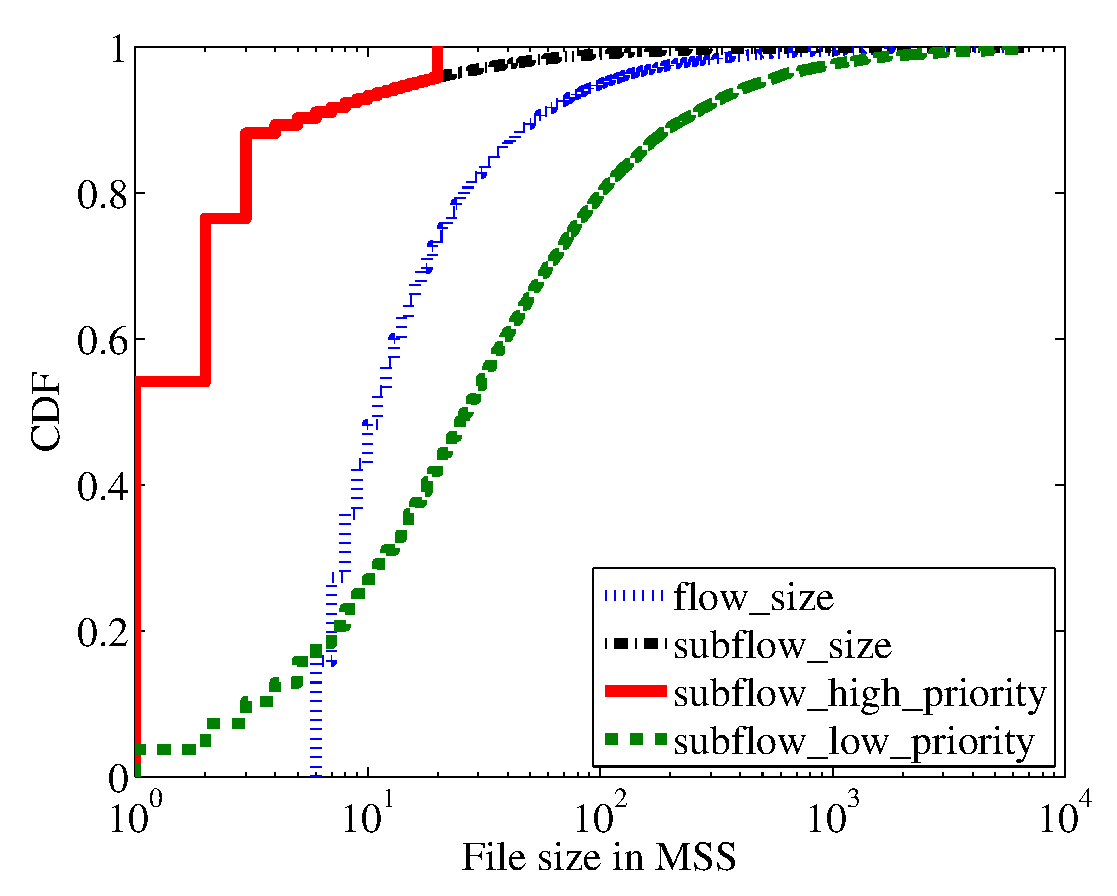
\includegraphics[width=0.495\textwidth]{./fig/wired/topology/mg1_cdf_bp_5_all.eps}}          
%  \caption{Network topology and flow size distribution}
%  \label{fig:wired_topology}
%\end{figure}


\subsubsection{Workload generation}\label{sec:workload}
Suppose that the bottleneck link has a capacity of C bits/s. The traffic demand, expressed as a bit rate, is the product of the flow arrival rate $\lambda$ and the average flow size $E[\sigma]$. The load offered to the link is then defined as:

\begin{equation}
\rho = \frac{\lambda E[\sigma]}{C}
\end{equation}

In all cases, the global load is controlled by tuning the arrival rate of requests. Thus, the congestion level increases as a function of the load. The flow arrivals follow a Poisson process, and the content requested is distributed according to a bounded Zipf distribution. Note that a bounded Zipf distribution is a discrete analog of the continuous bounded Pareto distribution, and Pareto is a heavy-tailed distribution usually adopted for modeling flows in the Internet. %Figure \ref{fig:wired_topology}(b) gives the flow size distribution used in the simulation. %Due to the fact that TCP traffic occupy mass of current Internet traffic, without loss of generality, TCP transfers are generated instead of UDP and FTP/GENERIC applications are applied in our simulation. 
 
%As the first step of study, we generate unidirectional traffic for simplicity. In our case, that is TCP traffic in terms of FTP/GENERIC applications directing from servers to clients (\textit{i.e.} from \{1, 2, 3, 4, 5\} to \{8, 9, 10, 11, 12\} in Figure \ref{fig:result1}).
Transfers are performed over TCP or UDP depending on the simulation. For each simulation set-up, we consider an underload and an overload regime, which correspond respectively to workloads of 8 and 15 Mb/s (80\% and 150\% of the bottleneck capacity). For TCP simulations, we use the GENERIC-FTP model of Qualnet, which corresponds to an unidirectional transfer of data. For UDP transfers, we use a CBR application model where one controls the inter-packet arrival time. The latter enables to control the exact rate at which packets are sent to the bottleneck. In both TCP and UDP cases, IP packets have a fixed size of 1500 bytes.


\subsection{EFD Internal Dynamics }


In this section, we present a detailed analysis of the way EFD manages flows. This is of utmost interest as it is a key distinguishing property of EFD as compared to other size-based scheduling policy. We focus on the following aspects:
\begin{itemize}
\item The evolution of the flow table size;
\item How traffic is split between the low and high priority queue.
\item  How connections are fragmented by the scheduler due to the insertion/removal process within the flow table;
\end{itemize}


% \subsection{Behavior Analysis}
% All simulations are performed lasting the same duration of 500 seconds in our experiments. Workload with two different throughput: 8Mbit/s and 20Mbit/s are generated in our simulation, producing underload ($\rho<1$) and overload ($\rho>1$) conditions respectively since the bottleneck link capacity is 10 Mbit/s. As the first step, it's interesting to study the behavior of EFD on how queue with limited maximum size grows, how flow table goes up and down, how the flow volumes are splitted and how flow sizes distribute in two virtual queues.

% In contrast to FIFO, LAS and RuN2C, flow splitting up is a particular phenomenon in EFD, showing critical effect on the behavior. It's evident that flows with different rates (either high rate or low rate) may exhibit quite distinguishable behavior on flow splitting up. Interestingly, it makes sense to investigate how rate affects the behavior, which is carefully studied in this section using CBR traffic with different rates. In addition, pursuiting how flow volumes distribute in two virtual queues with different priorities can help to better understand how EFD works. 

\subsubsection{Flow table}

Due to the discarding mechanism of flow entries within the flow table in EFD, a flow entry exists in the flow table only if at least one packet of the flow is present in the queue. As stated in Section \ref{sec:efd_alg}, an important consequence is that the flow table size is bounded by the physical queue size in packets\footnote{In most if not all active equipments -- routers, access points -- queues are counted in packets and not in bytes.}. %Indeed, in the worst case, there is as many entries as distinct flows in the physical queue, each with one packet.
%Therefore, it is clear that flow table size is upper bounded by queue size while it mainly depends on the unbouned number of flows on high speed link in LAS, 

For the TCP workload, we plot in Figure \ref{fig:dynamics} the instantaneous queue size and the instantaneous flow table size in underload and overload. Remind that the buffer size is 300 packets in our experiments. Figure \ref{fig:dynamics} reveals that both flow table and packet queue grow up as the traffic intensity increases, but the table size is consistently below the queue size. Even in the overload case, the flow table size remains fairly small. We further investigate this issue in Section \ref{sec:table_size}.%changes from underload to overload. Especially, packet queue reaches full at most time in overload case.  

\begin{figure}[ht]
  \centering
  \subfigure[workload of 8Mbit/s (underload)]{\label{fig:wifib-01}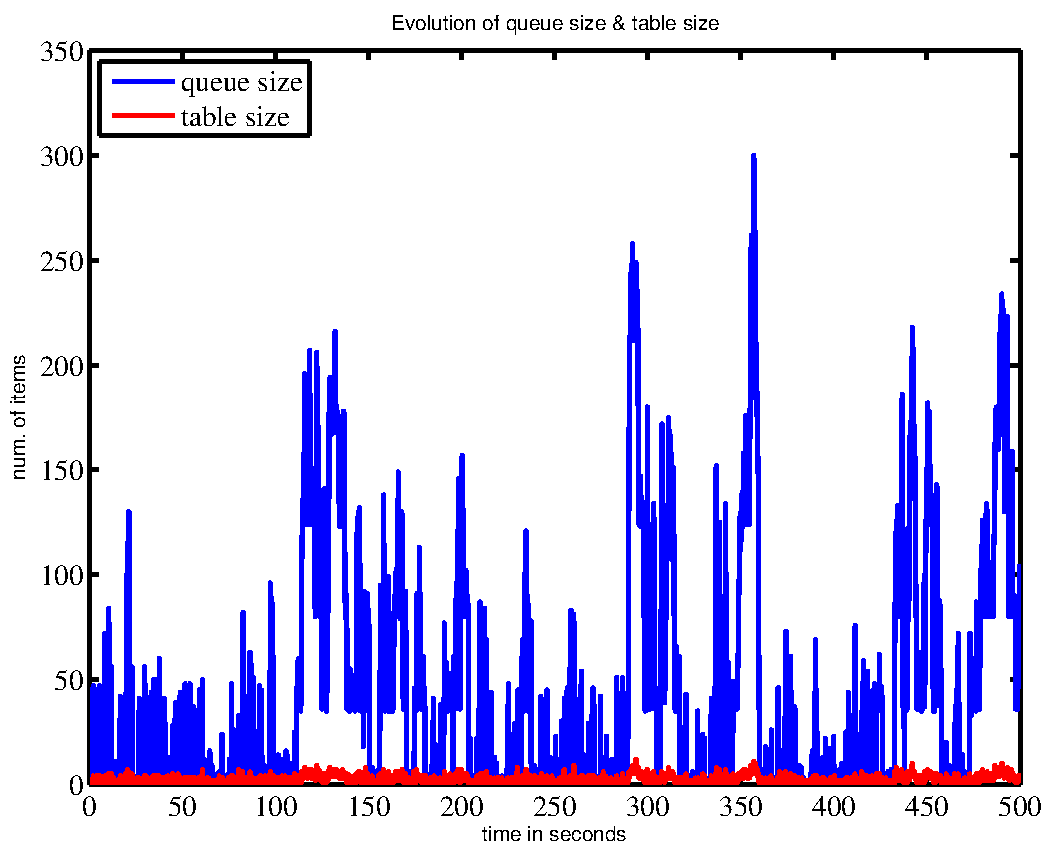
\includegraphics[width=0.49\textwidth]{./fig/wired/internal_dynamics/lq_8}}
  \subfigure[workload of 15Mbit/s (overload)]{\label{fig:wifia-01}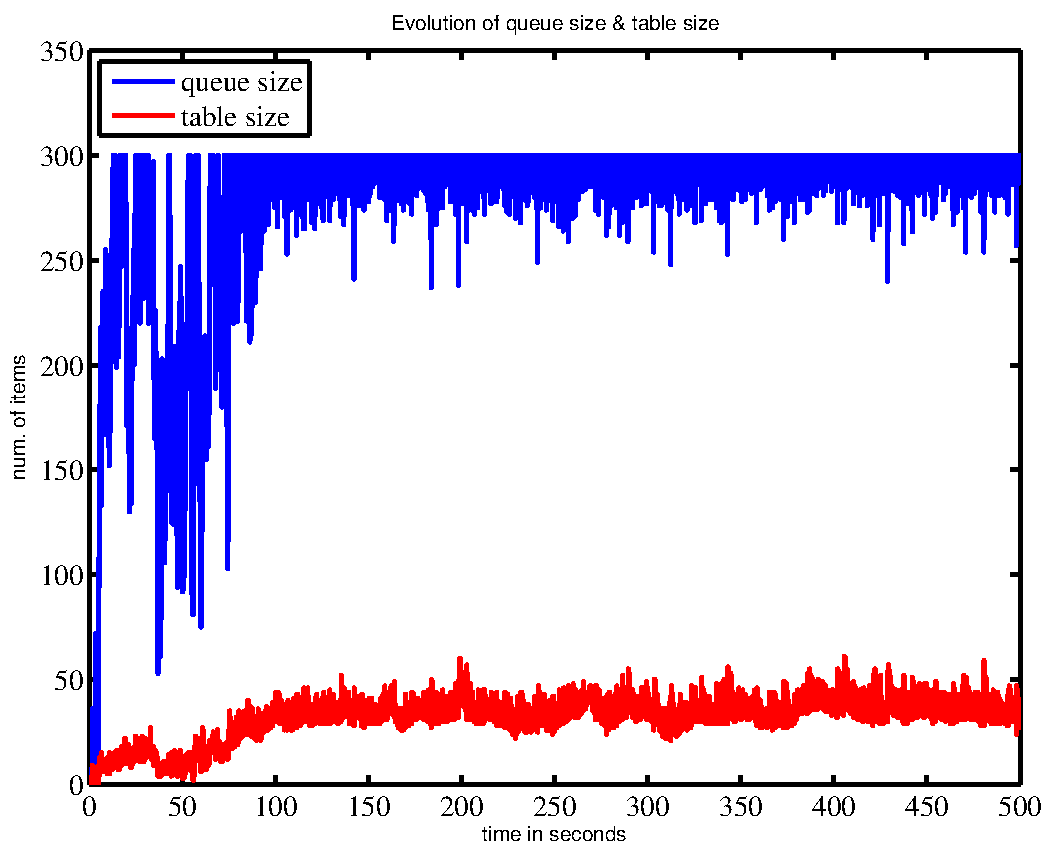
\includegraphics[width=0.49\textwidth]{./fig/wired/internal_dynamics/lq_20}}  
  \caption{Queue size \& Table size}
  \label{fig:dynamics}
\end{figure}

\subsubsection{Virtual queue sizes}

As EFD features two queues with high and low priority respectively, Figure \ref{fig:queue_evo} depicts the evolution of the two virtual queue sizes, together with the overall queue (\textit{i.e.} physical queue) size in underload and overload. One clearly sees that the low priority queue carries the bulk of the traffic. It is in line with our expectation as we want the high priority queue to be lightly loaded so that packets can be served as fast as possible, in order to grant short flows with low mean response times. While the bufferbloat phenomenon is often presented as the persistence of large queues that degrade the performance of every flow, we see that with the size-based scheduling approach, we can have simultaneously high buffer occupancy while still low response to young/short flows.


\begin{figure}[ht]
  \centering
  \subfigure[workload of 8Mbit/s (underload)]{\label{fig:wifib-01}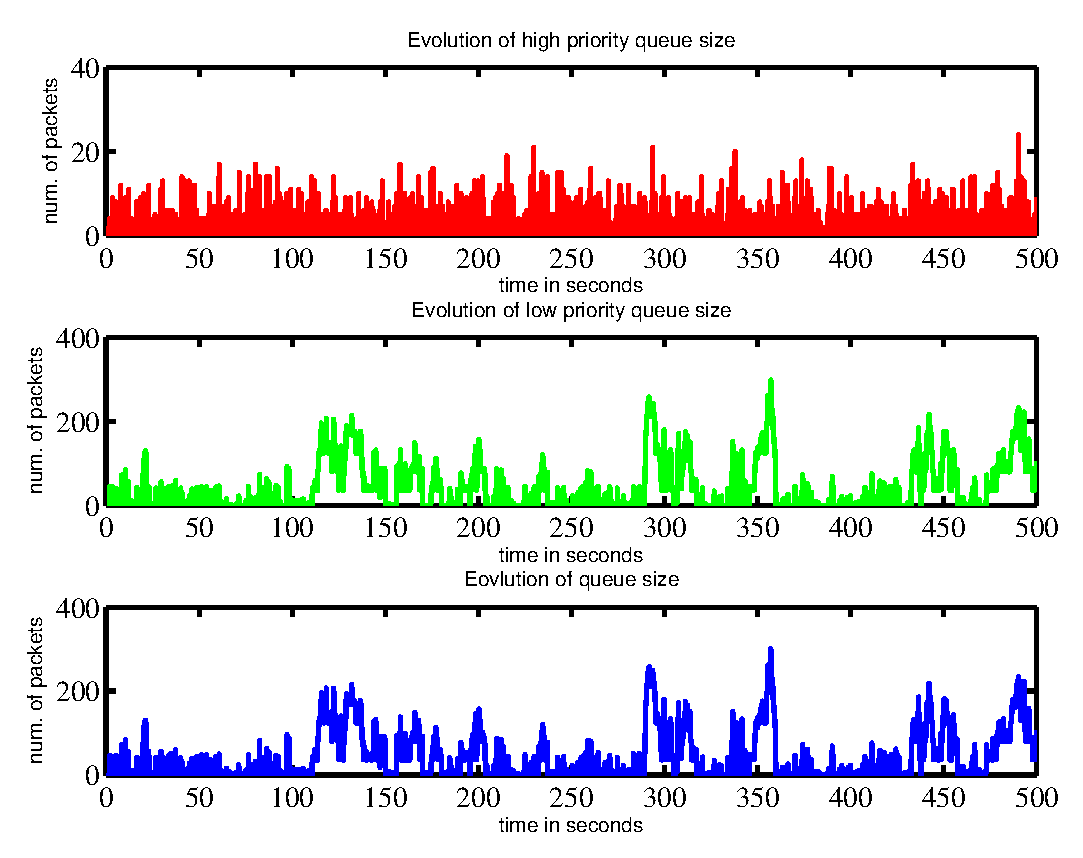
\includegraphics[width=0.49\textwidth]{./fig/wired/internal_dynamics/slpktsub_8.eps}}
  \subfigure[workload of 15Mbit/s (overload)]{\label{fig:wifia-01}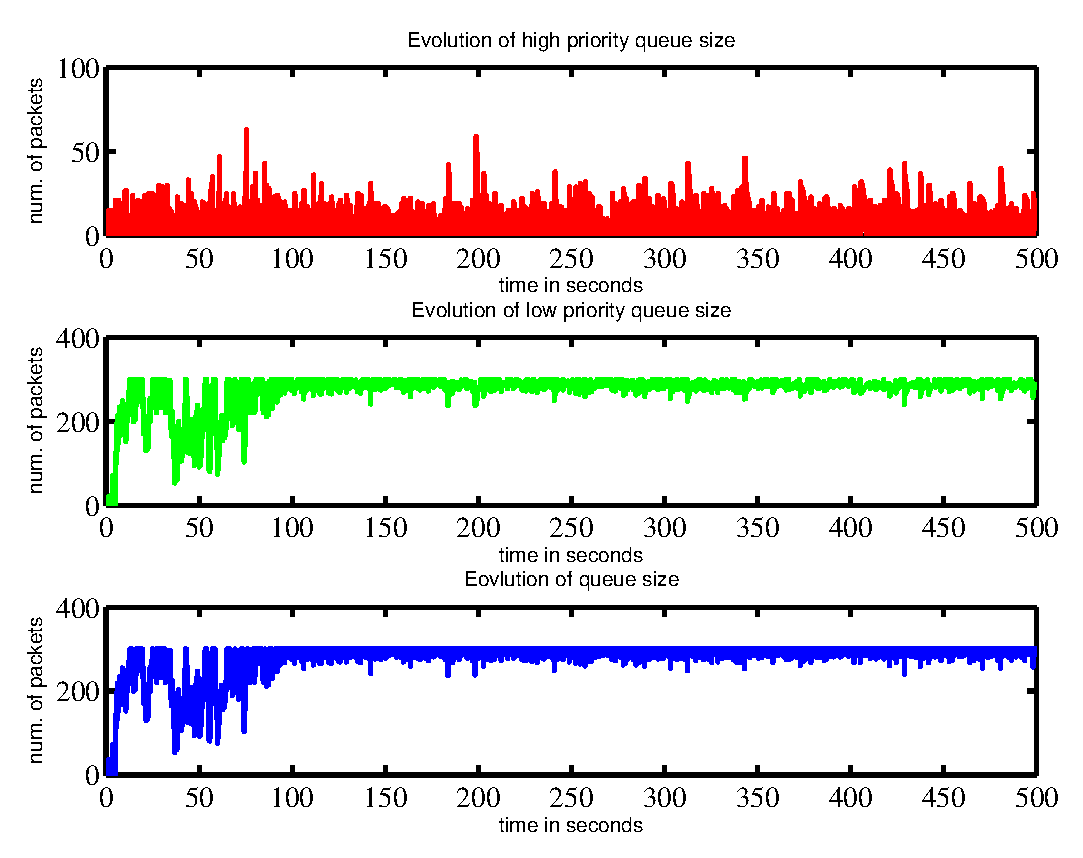
\includegraphics[width=0.49\textwidth]{./fig/wired/internal_dynamics/slpktsub_20.eps}}  
  %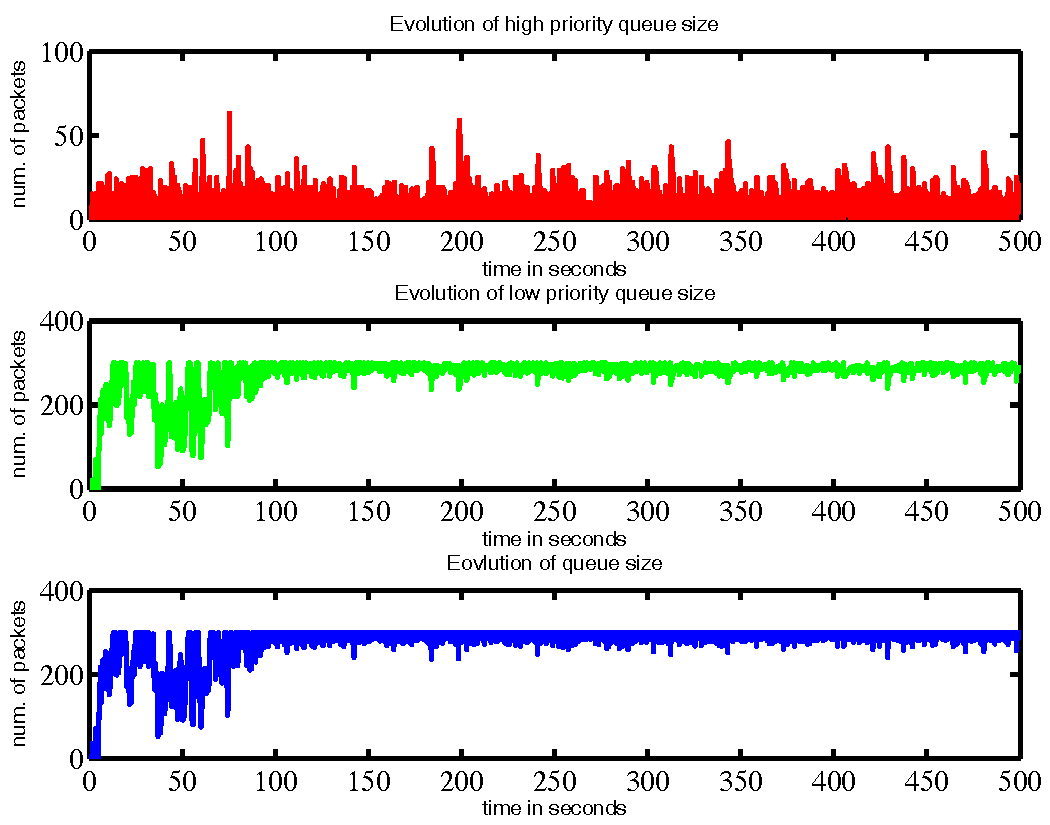
\includegraphics[width=0.4\textwidth]{./fig/internal_dynamics/slpktsub_20}
  \caption{Evolution of high and low priority queue size  in both underload and overload.}
  \label{fig:queue_evo}
\end{figure}


\subsubsection{Flow fragmentation} \label{sec:fragmentation}

With EFD, a connection can be fragmented into many flows - each one is treated as fresh by the scheduler. In addition, the packets of one of these flows might be partly serviced in high priority or low priority queue: the first \textit{th} packets are serviced by the high priority queue and the rest by the low priority queue. We call this phenomenon ``flow fragmentation''. It is in clear contrast to FIFO, LAS and RuN2C.

In practice, several phenomena can lead to break a connection into many fragments. For instance,  during connection establishment, the TCP slow start algorithm limits the number of packets in flight so that it does not continuously occupy the buffer. This is however not a problem, as those flows are smaller than $th$ and thus young  TCP transfers will receive a high priority. If the flow lasts longer and it is effectively able to use its share of the capacity, then the connection will eventually occupy  the buffer without interruption and therefore stay in the flow table. Figure \ref{fig:seg8} illustrates such a scenario. It is apparent that, as the connection size increases, the number of fragments tends to reach a limit so that, for the longest connections, a small number of fragments correspond to many packets.

%"Fragmentation" is often used to describe the phenomenon in which data packet for transmission is shaped by cutting it into certain amount of small packets due to the limitation of MTU in the network. Here we borrow this concept for flows instead of packets, meaning that a single flow is cut into several pieces for some reason.  

%Figure \ref{fig:result5} shows the flow fragmentations in the simulation when the EFD scheduling policy is applied over the bottleneck link. As we know that, EFD's entry-discarding mechanism can effectively restrain flow table from rapidly growing by bounding it with the finite buffer size, but result in flow fragmentation at the same time. In our context, flow fragmentation means that one flow (or connection) is splitted into several blocks, leading to entry recreation time after time and more packet incorporations in high priority queue. From Figure \ref{fig:result5}(a), it's evident that the mass (90th percentage) of the connection fragmentations are distributed in the range of [6, 37], while the number of the fragmentations with dominant values are carried by few coutable connections.

%Figure \ref{fig:seg8} depicts the average number of flows per connection. Those flows are also called segments.  We observe that the average number of segments increases with the connection size, which means that long connections are more prone to be fragmented. This figure calls for several remarks. First, one can notice that for small transfer sizes, the number of segments is larger than the number of data packets to be transmitted. This is because of the TCP control packets. Let us consider the simplest case: a transfer of a single MSS packet. In this case, in the server to client direction, which is the one interest, the scheduler will see one SYN/ACK packet, one data packet and one FIN packet. Ideally, each packet is separated from the other by one RTT. Hence, from the scheduler viewpoint, it is likely that they generate 3 distinct flows or segments. When the transfer size increase, the number of segments also increase but at a smaller speed, as one lays below the bissector line, but still quite close to it (even if the log-log scale might be misleading). One thus have the feeling that each segment corresponds to a modest number of packets. If this were the case, then most of the packets would be directed to the high priority queue, and EFD would degenerate to FIFO. This is however not the case as we have seen in Figure \ref{fig:queue_evo} that the short queue was significantly smaller than the large queue. 

\begin{figure}[ht]
  \centering
  %\subfigure[Distribution of flow fragmentation]{\label{fig:wifib-01}\includegraphics[width=0.49\textwidth]{./fig/seg_cdf_8.eps}}
  %\subfigure[Relationship between flow size and fragmentation]{\label{fig:wifia-01}\includegraphics[width=0.49\textwidth]{./fig/segment_8.eps}}  
  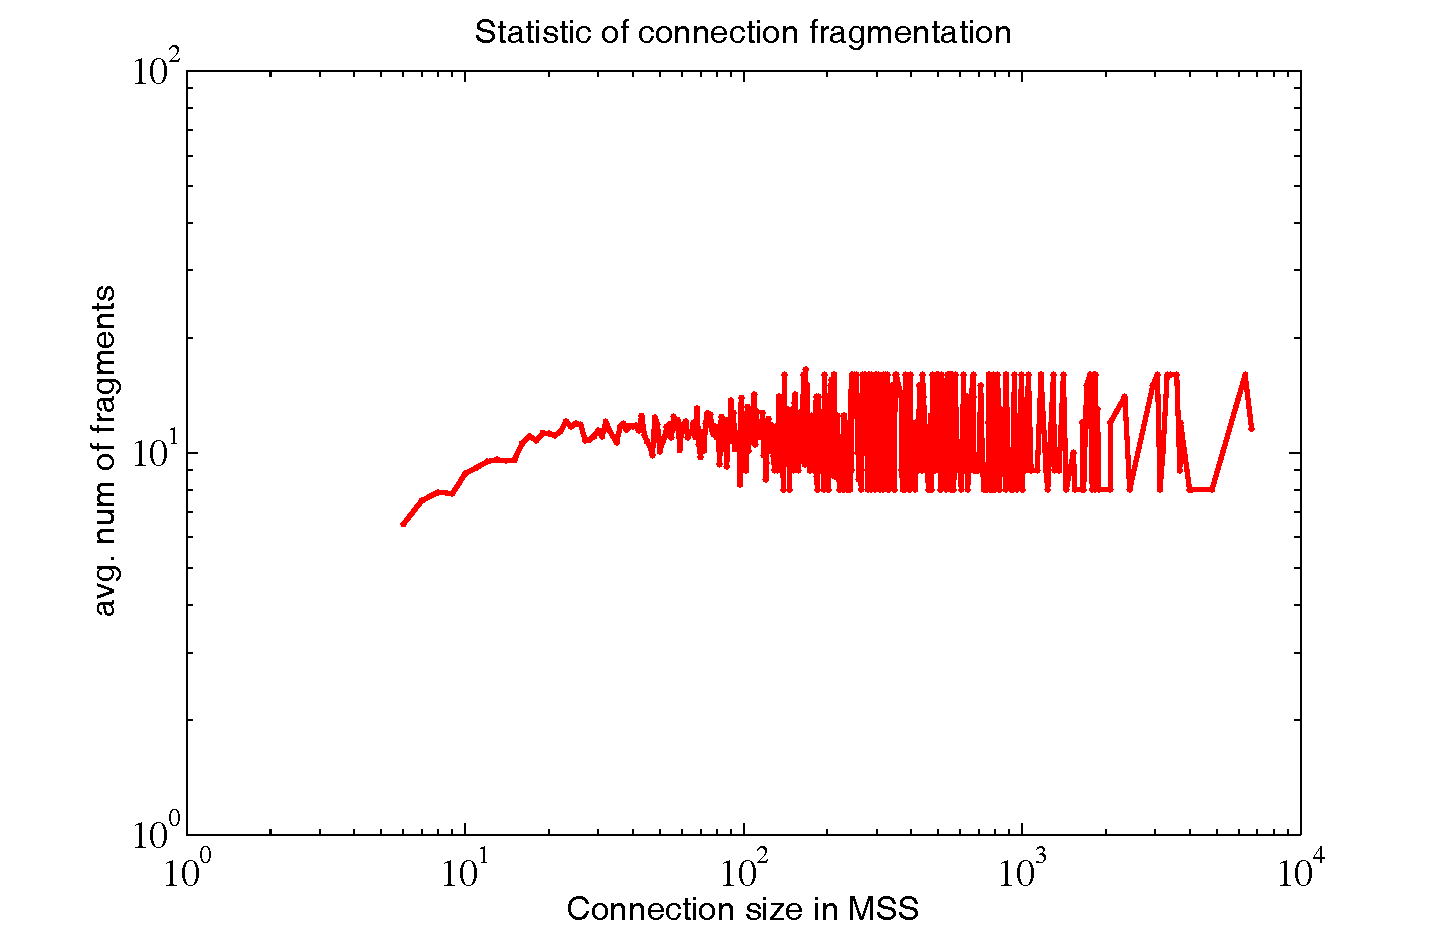
\includegraphics[width=0.7\textwidth]{./fig/wired/internal_dynamics/segment_8}
  \caption{Number of segments per connection - workload of 8Mbit/s}
  \label{fig:seg8}
\end{figure}

\begin{figure}[ht]
  \centering
%  \subfigure[Comparison between flows and subflows - cdf]{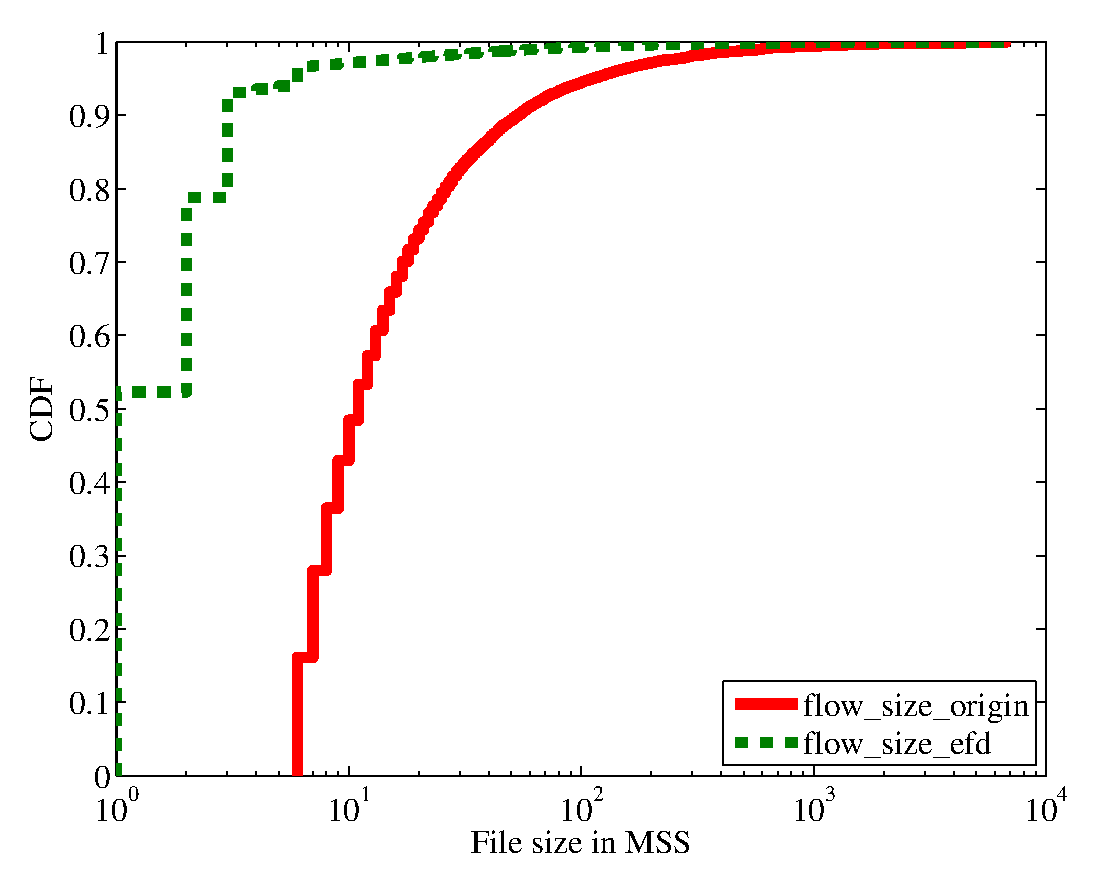
\includegraphics[width=0.495\textwidth]{./Part1/Chapter4/fig/chapter_one/mg1_cdf_bp_5.eps}}
%  \subfigure[Comparison between flows and subflows - prctile]{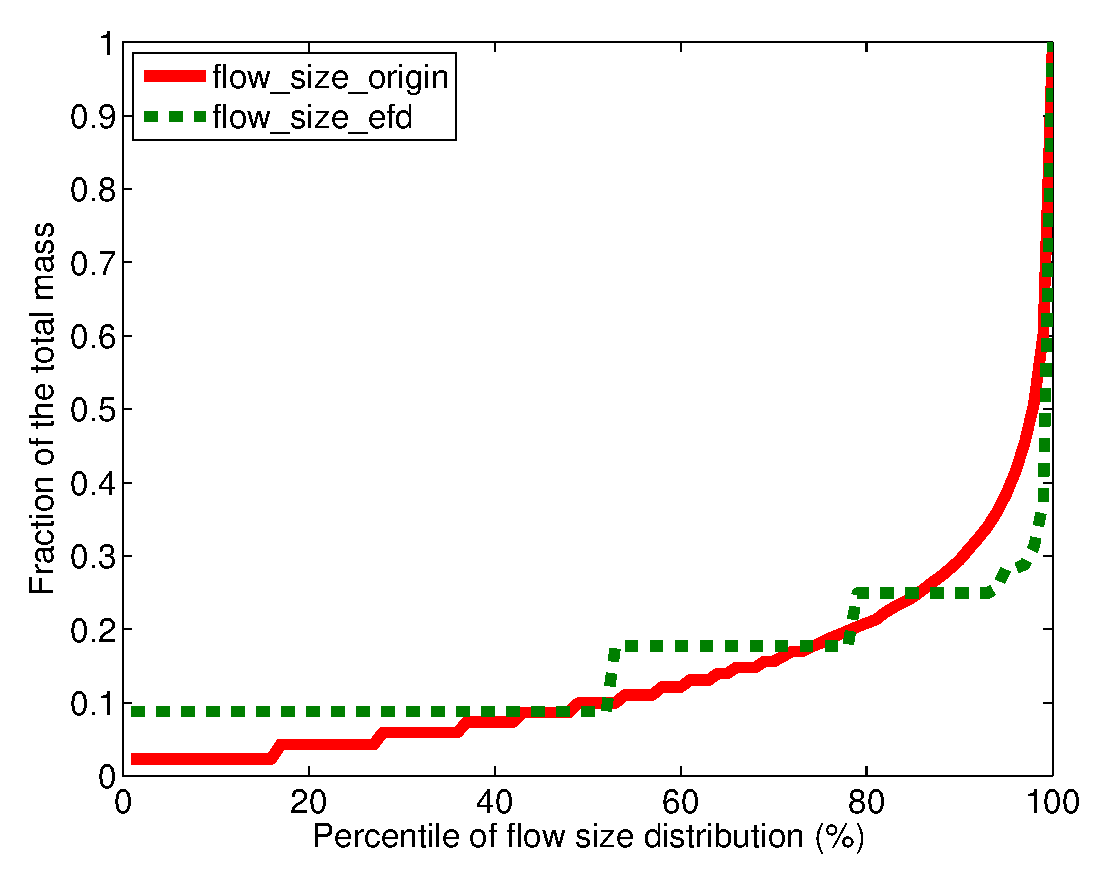
\includegraphics[width=0.495\textwidth]{./Part1/Chapter4/fig/chapter_one/mg1_prctile_bp_5.eps}}	
%  \subfigure[Subflows in two queues - cdf]{\includegraphics[width=0.495\textwidth]{./Part1/Chapter4/fig/chapter_one/mg1_cdf_queue_5.eps}}  
%  \subfigure[Subflows in two queues - prctile]{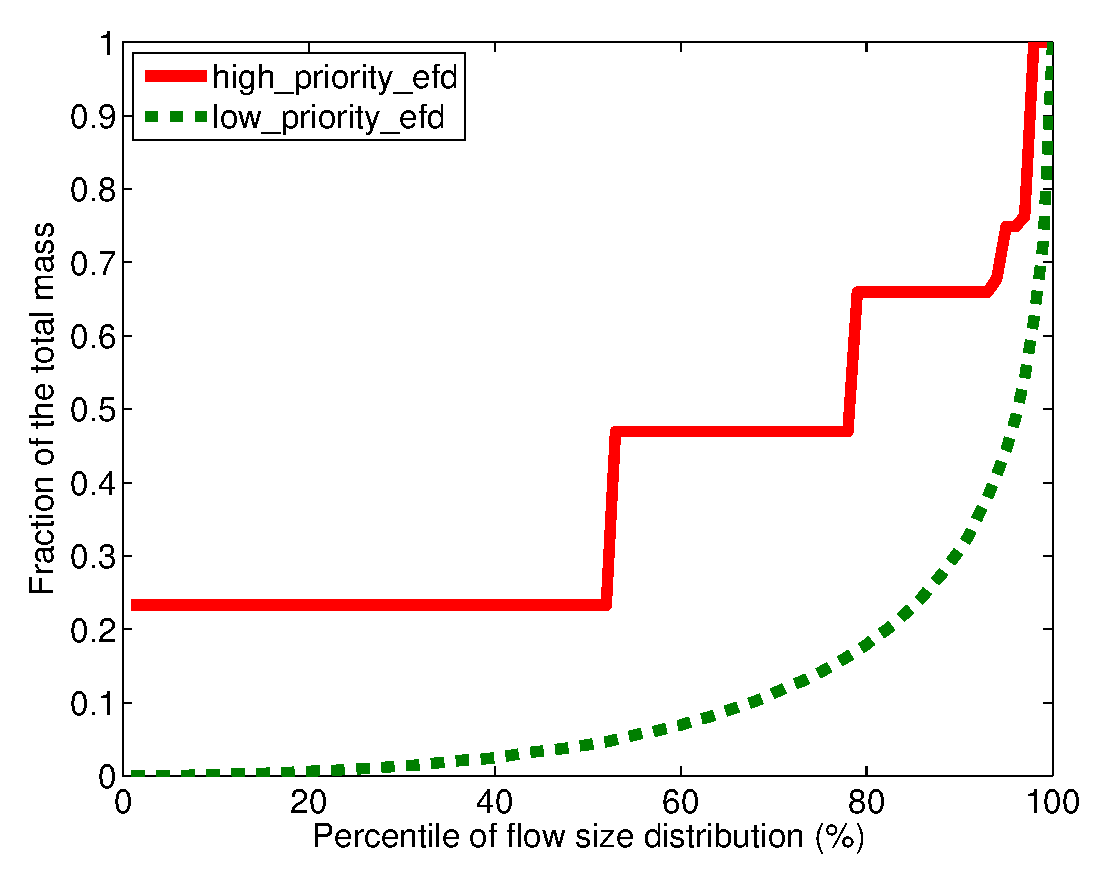
\includegraphics[width=0.495\textwidth]{./Part1/Chapter4/fig/chapter_one/mg1_prctile_queue_5.eps}}  	
  \subfigure[CDF]{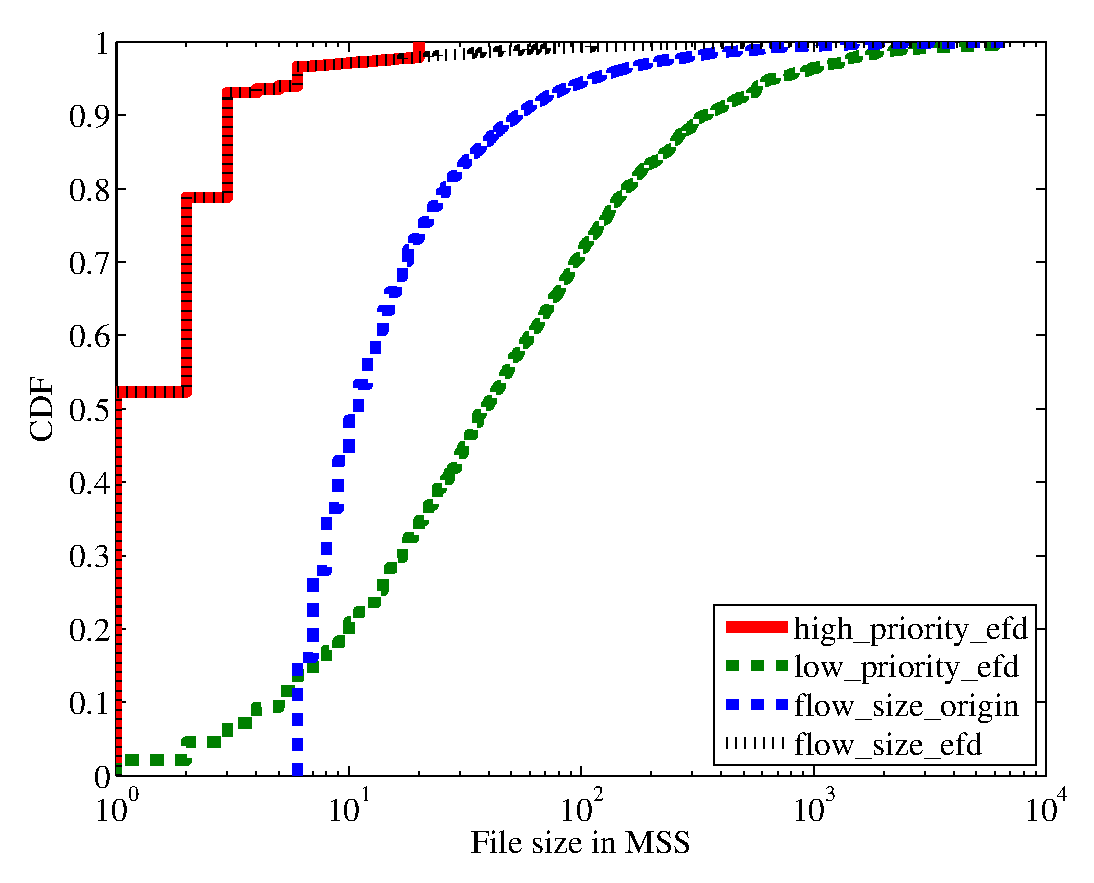
\includegraphics[width=0.495\textwidth]{./fig/analysis/mg1_cdf_bp_5_all.eps}}
  \subfigure[Mass-Weighted Distribution]{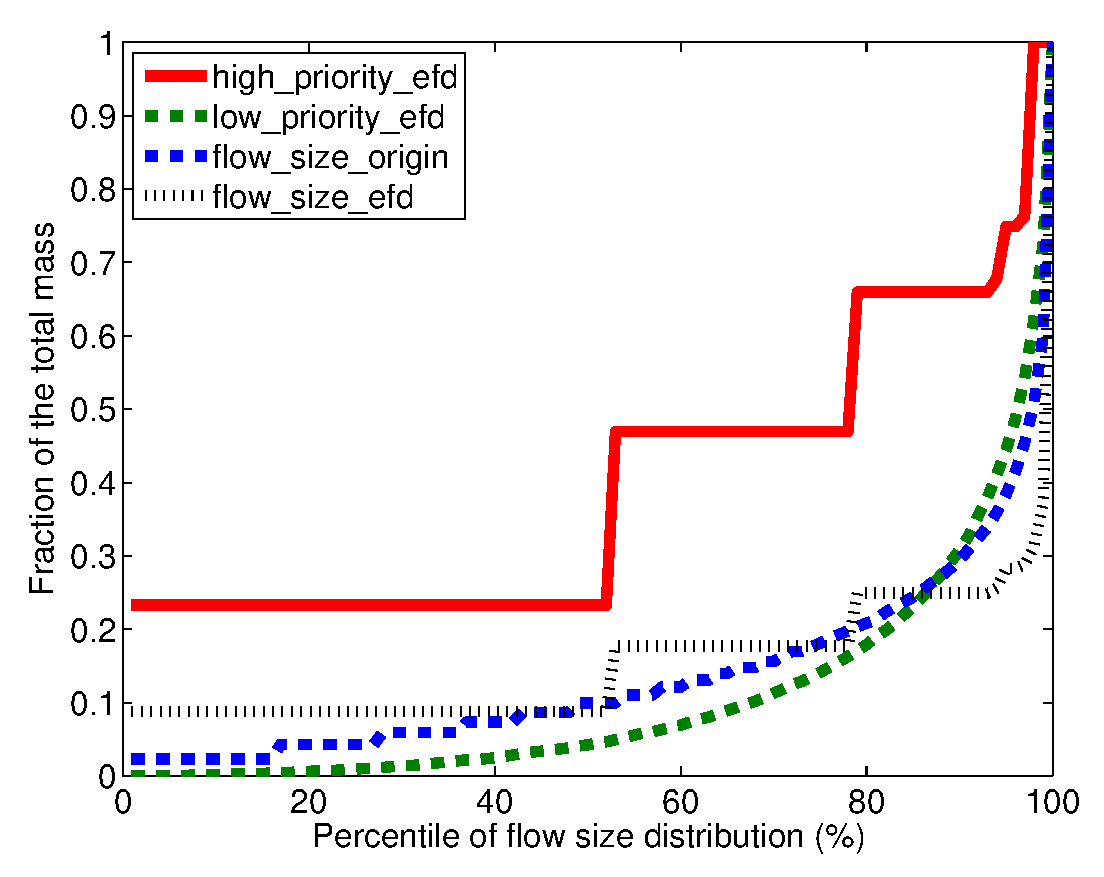
\includegraphics[width=0.495\textwidth]{./fig/analysis/mg1_prctile_bp_5_all.eps}}          
  \caption{Flow and subflow size distribution, workload of 5Mbit/s}
  \label{fig:flow_subflow}
\end{figure}

In order to illustrate how a flow is split into subflows under EFD, we report the flow size and subflow size distributions in Figure \ref{fig:flow_subflow}  for an experimental setup similar to the one in Figure \ref{fig:wired_topology}.  %Ideally, EFD was designed to favor short and persistent low rate flows. In reality, the TCP congestion control policy restricts the packets' arrival behavior, beginning with slow start in general by sending packets in flights and recovering in the manner of timeout (RTO) or fast retransmit/recovery (FR/R) in case of loss event. Furthermore, even the packets sent in the same flight are not always observed to arrive to the scheduler at the same time since they may cross traffic over the same or different paths. 
We observe from Figure \ref{fig:flow_subflow}(a) that, flows are prone to be split into many extremely small subflows, in which subflows with size less than or equal to 3 packets make up around 90\% of subflows, given that the original flow size distribution is Zipfian. In addition, subflow size distribution in the low priority queue (black dotted line) retains the heavy tail property as flow size distribution shown in mass-weighted distribution in Figure \ref{fig:flow_subflow}(b), but exhibits smaller variability in contrast to the original flow size distribution (blue dotted line). 


To get a better understanding of the way EFD partitions traffic among the low and high priority queues, we present in Figure \ref{fig:flow_dist}(a) the distributions of transfer sizes in both queues. Due to the way EFD operates, a given transfer is broken in possibly many flows or fragments from the scheduler's viewpoint. In addition, the \textit{th} first packets of each flow are serviced by the high priority queue and the rest, if any by the low priority queue. For each TCP transfer, we sum the total number of packets serviced at the high priority queue and the low priority queue respectively over all the segments of this transfer. We further add the original distribution of transfer sizes (at the TCP layer). We observe from  Figure \ref{fig:flow_dist}(a) that the distribution of flow sizes  in the low priority queue consists of larger flows than in the high priority queue, even though long transfers can be partially or fully serviced in the high priority queue. This behavior of EFD is in contrast to Run2C, which is another Multi-Level Processor Policy, with the same number of levels and policy at each, but that adopts a fixed threshold per transfer: the first \textit{th} packet goes to the high priority queue while the rest goes to the low priority queue -- see  Figure \ref{fig:flow_dist}(b). Clearly, EFD imposes a higher load on the high priority queue as compared to Run2C. This should not be interpreted as a drawback of EFD as compared to Run2C since it allows EFD to account for rates and not only for volumes, as we further illustrate with the UDP experiments in Section \ref{sec:multi_media}. 

\begin{figure}[ht]
  \centering
  \subfigure[EFD]{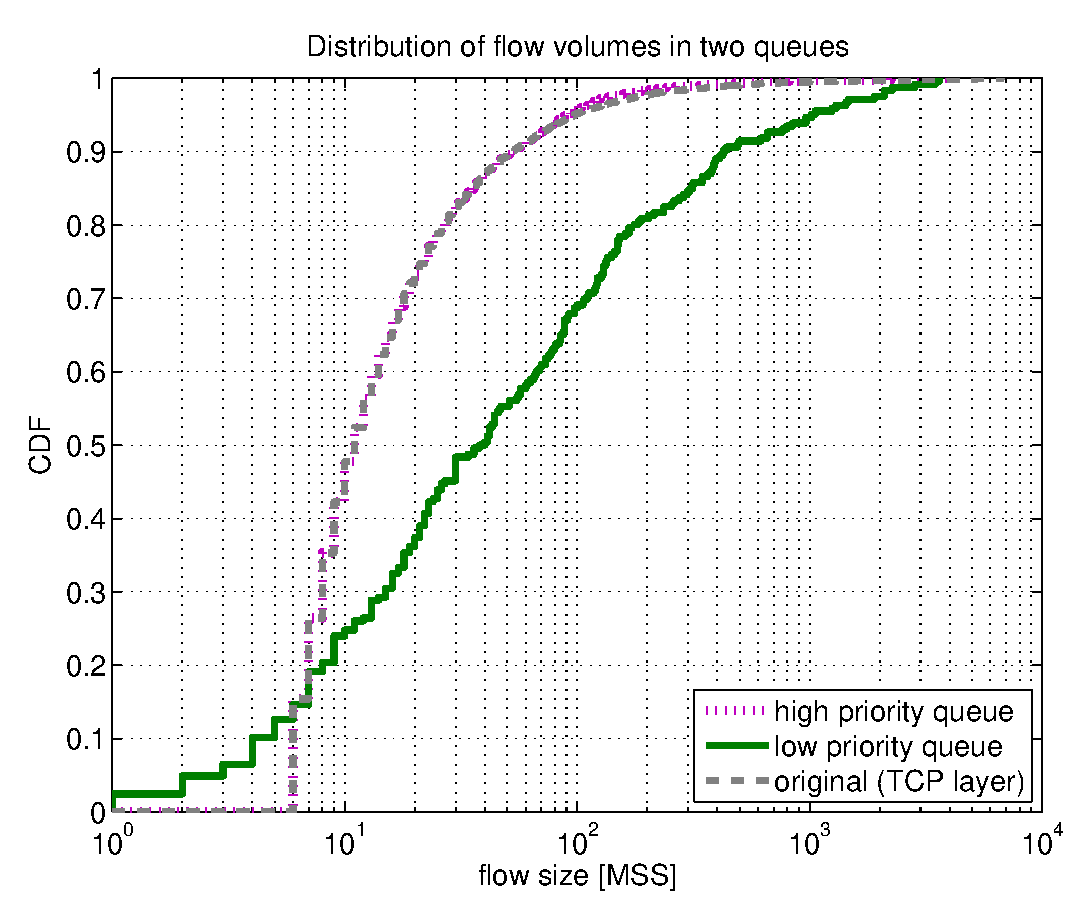
\includegraphics[width=0.49\textwidth]{./fig/wired/internal_dynamics/cumulated_cdf_8}}
 \subfigure[RuN2C]{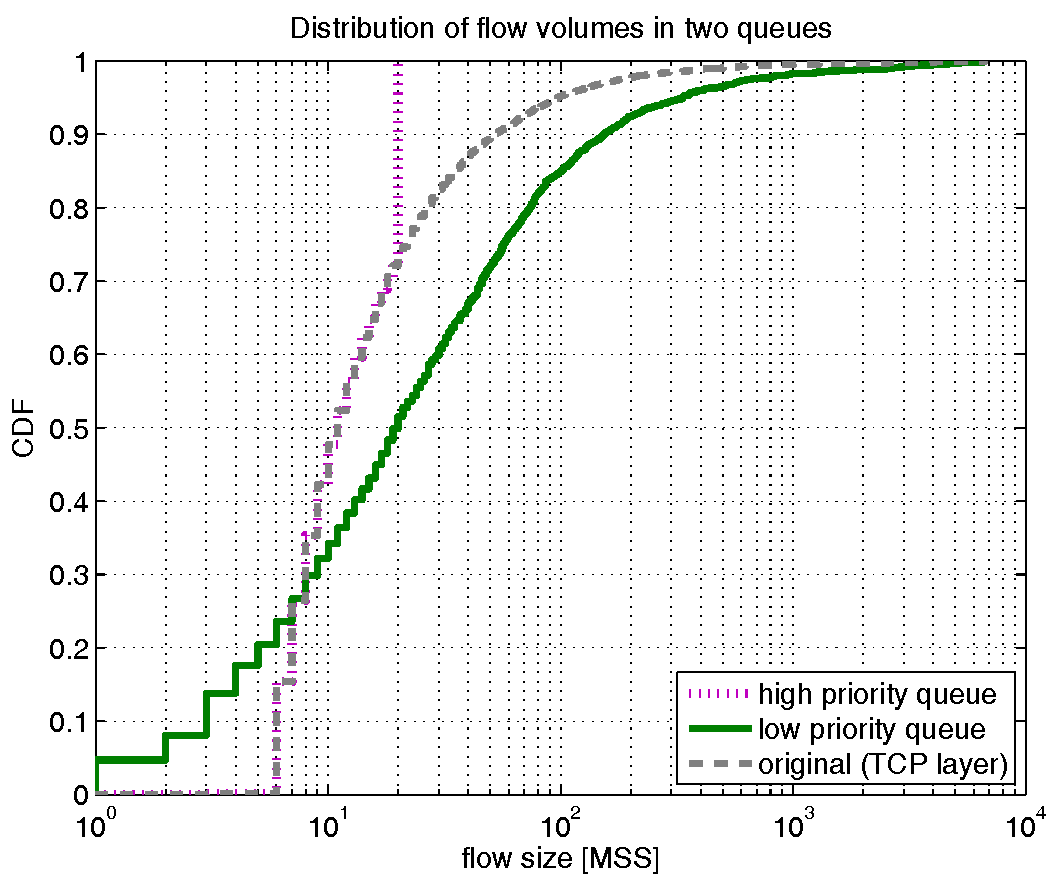
\includegraphics[width=0.49\textwidth]{./fig/wired/internal_dynamics/run2c_isolated_cdf_8}}
  \caption{Distribution of flow volumes in two queues - workload of 8Mbit/s}
  \label{fig:flow_dist}
\end{figure}

\subsection{Performation Evaluation}
We compare the performance of EFD to other scheduling policies. Our objective is to illustrate the ability of EFD to fulfill the 4 objectives listed in the introduction, namely (i) low bookkeeping cost, (ii) low response time to small flows, (iii) avoiding lock-outs, (iv) protecting long lasting delay sensitive flows.%differentiating flows based on volumes but also based on rate/burstiness. 

To illustrate the first 3 items, we consider a TCP workload with homogeneous transfers, \textit{i.e.}, transfers that take place on paths having similar characteristics. For the last item - protecting long lived delay sensitive flows - we add a UDP workload to the TCP workload in the form of a CBR traffic,  in order to highlight the behavior of each scheduler in presence of long lasting delay sensitive flows. %For the last item - taking rate into account - we consider a UDP workload consisting of CBR transfers, that allows to precisely control the rate at which the sender is sending data, and thus highlight the behavior of each scheduler when senders have different sending rates.

%We focus on two important metrics: the size of the flow list size and the response time.


%The objective of the experiments is to investigate the benefits of EFD in the form of granting short flows low response time while limiting the starvation to long flows and taking advantage of flow rate for differentiated service with low resource consumption. we place our emphasis on the study of overhead of flow state keeping and mean response time of flows. In addition, the throughput issue is also examined. 

 

\subsubsection{Overhead of flow state keeping}\label{sec:table_size}
The approaches to maintain the flow table in the size-based scheduling policies proposed so far can be categorized as follows: %, several approaches have been proposed to maintain the flow list:
\begin{itemize}
 \item Full flow table approach as in LAS \cite{Rai04size-basedscheduling}. An argument in favor of keeping one state per active flow is that the number of flows to handle remains moderate as it is expected that such a scheduling policy be implemented at the edge of the Internet.
\item No flow table approach: an external support is provided to the scheduler, either at the end-hosts by modificaitons of the transport layer \cite{Avrachenkov04Run2c} or by some intermediate boxes, as in the case of a DiffServ scheme \cite{Noureddine02improvingthe}, that marks the packets. The extent of the changes required to the Internet architecture prevents the deployment of such approaches in a near future.
%an external mechanism marks the packets or the information is implicit (coded in the TCP SEQ number in Run2C) \cite{Avrachenkov04Run2c,Noureddine02improvingthe}
\item Probabilistic approaches:  a test is performed at each packet arrival for flows that have not already be incorporated in the flow table \cite{DivakaranCAP10,Kortebi04Xprotect,Psounis05Sift}. The test is calibrated in such a way that only long flows should end up in the flow table. Still, false positives are possible. Several options have been envisaged to combat this phenomenon especially, a re-testing approach \cite{Psounis05Sift} or an approach where the flows in the flow table are actually considered as long flows once they have generated more than a certain amount of packets/bytes after their initial insertion \cite{DivakaranCAP10}.
\item EFD deterministic approach:  the EFD approach is fully deterministic as flow entries are removed from the flow table once they have no more packet in the queue. 
\end{itemize}

In this section, we compare all the approaches presented except the ''No flow table approach'' for our TCP workload scenario. We consider one representative of each family: LAS, X-Protect and EFD. We term X-Protect a Multi-Level Processor Scheduling policy that maintains two queues, similarly to Run2C, but uses the probabilistic mechanism proposed by Kortebi \cite{Kortebi04Xprotect} to track long flows. As for the actual scheduling of packets, X-Protect mimics Run2C based on the information it possesses. If the packet does not belong to a flow in the flow table nor passes the test, it is put in the high priority queue. If it belongs to a flow in the flow table, it is put either in the high priority queue or in the low priority queue, depending on the amount of bytes sent by the flow. We use a threshold f 30KB, similar to the one used for EFD.

%As we have mentioned before, probability mechanism can be an option for the differentiation between short and long flows, which is originally proposed for admission control in Cross-protect \cite{Kortebi04Xprotect}. It sees potential improvement since we may only need to keep state information for long flows which are quite few compared to the total number of flows. In order to better understand the overhead of flow state keeping, a scheduling discipline "X-Protect" based on this probability mechanism is deployed in our simulation for comparison with LAS and EFD. Instead of keeping flow state for all active flows in LAS, X-Protect only maintains state information for those flows who pass the probability test, resulting in less resource consumption in terms of flow table size. In addition, X-Protect adopts the same two queues approach and the same buffer management strategy as EFD, while it cleans up the flow entries in the flow table periodically as LAS without entry-discarding mechanism. 

%Concerning the memory consumption, there are several aspects to analize. First of all, examining the evolution of flow table sizes over time series in the whole duration is kind of straightforward, which can be roughly tracked by simply printing out the instantaneous flow table size at the critical time points, such as the event time at which a flow entry is added to or removed from the table, or event time at which a new packet arrives or dequeues, and so on. It makes sense since the time slot between two adjacent events is quite narrow compared to the whole simulation time. 

The evolution of  flow table size over time for load of 8Mbit/s (underload) and 15Mbit/s (overload) are shown in Figure \ref{fig:result11}. For LAS and X-Protect, the flow table is visited  every 5 seconds  and the flows that have been inactive for 30 seconds are removed. %The slope of the curves between two cleaning events, implicitly indicates the constant flow arrival rate of the Poisson process used in the simulation.

\begin{figure}[ht]
  \centering
  \subfigure[workload of 8Mbit/s (underload)]{\includegraphics[width=0.49\textwidth]{./fig/wired/flow_table/evo_8}}
  \subfigure[workload of 15Mbit/s (overload)]{\includegraphics[width=0.49\textwidth]{./fig/wired/flow_table/evo_15}}  
  \caption{Evolution of flow table size over time}
  \label{fig:result11}
\end{figure}

%\begin{figure*}[ht!]
%  \centering
%  \subfigure[workload of 8Mbit/s (underload)]{\includegraphics[width=0.49\textwidth]{./fig/wired/evo_8}}
%  \subfigure[workload of 15Mbit/s (overload)]{\includegraphics[width=0.49\textwidth]{./fig/wired/evo_15}}  
%  \caption{Evolution of flow table size over time}
%  \label{fig:result11}
%\end{figure*}

We observe how X-Protect roughly halves the number of tracked flows, compared to LAS. By contrast, EFD reduces it by one order of magnitude. The reason why X-Protect offers deceptive performance is the race condition that exists between the flow size distribution and the probabilistic detection mechanism. Indeed, even though a low probability, say 1\%, is used to test if a flow is long, there exists so many short flows that the number of false positives becomes quite large, which prevents the flow table from being significantly smaller than in LAS. The histograms in Figure \ref{fig:result12} confirm the good performance of EFD in underload and also overload, as EFD keeps the flow table size to a few 10s of entries at most. Note that this is clearly smaller than the actual queue size (300 packets) that constitutes an upper bound on the flow table size in EFD as explained before. We also report the mean value and the 95\% level confidence interval of the flow table size over 1000 seconds simulation for both load conditions in Table \ref{tab:flow_table_size}. 
  %, benefitting from the probability mechanism for flow differentiation. However, it's still far away from our expection since the average flow table size can finally reach a small order of magnitude if flows can be well differentiated as short and long ones. In contrast to LAS and X-Protect, thanks to the entry-discarding mechanism, EFD sees encourging and considerable improvement with quite small overhead of flow state keeping. Precisely, the average flow table size keeps small in underload while it increases a bit in overload. 


%The statistics of memory consumption (in terms of flow table sizes in our case) in different scheduling policies (LAS, X-Protect and EFD) can be appropriately characterized with the method of weighted-average. Suppose that each existing flow table size $l_{i}$ lasts for the duration $\Delta t_{i}$, then the average flow table size $L_{avg}$ can be calculated in a weighted way, that is $L_{avg}$=$\frac{\sum^N_{i=1} l_{i}\Delta t_{i}} {\sum^N_{i=1} \Delta t_{i}}$, in which $N$ is the space size of all possible value of flow table sizes in one simulation. Therefore, this value $L_{avg}$ can be used to generally represent the memory consumption from the statistical point of view. Table \ref{tab:value} in the following shows these values what we have obtained from the simulation. In addition, the frequency of each unique flow table size can be presented as the division of the corresponding cumulated time duration and the total time period, which can be illustrated in the form of histogram shown in Figure \ref{fig:result12}.

%From Table \ref{tab:value}, we found that X-Protect roughly cuts the overhead of flow state keeping into half compared to LAS, benefitting from the probability mechanism for flow differentiation. However, it's still far away from our expection since the average flow table size can finally reach a small order of magnitude if flows can be well differentiated as short and long ones. In contrast to LAS and X-Protect, thanks to the entry-discarding mechanism, EFD sees encourging and considerable improvement with quite small overhead of flow state keeping. Precisely, the average flow table size keeps small in underload while it increases a bit in overload. 

% \begin{table*}[ht]
% 		\centering
%     \begin{tabular}{ | c | c | c | c | c | c |}
%     \hline
%     & FIFO & LAS & X-Protect & RuN2C & EFD \\ \hline
%     8Mbit/s & - & 389.988447 & 174.777213 & - & 2.479975  \\ \hline
%     10Mbit/s & - & 473.297309 & 214.915498 & - & 2.843578  \\ \hline
%     20Mbit/s & - & 988.913109 & 558.939708 & - & 31.089862 \\ \hline
%     \end{tabular}
%     \caption{Average flow table sizes}
%     \label{tab:value}  
% \end{table*}

\begin{figure}[ht]
  \centering
  \subfigure[workload of 8Mbit/s (underload)]{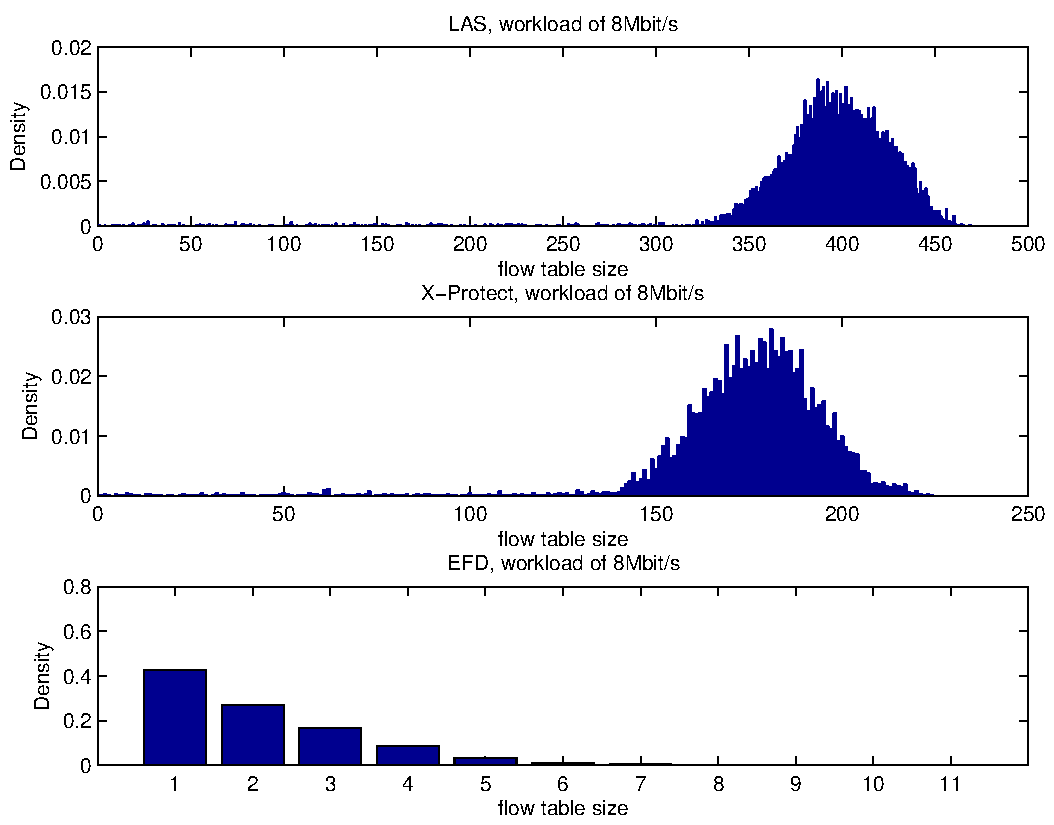
\includegraphics[width=0.49\textwidth]{./fig/wired/flow_table/density_8}}
  \subfigure[workload of 15Mbit/s (overload)]{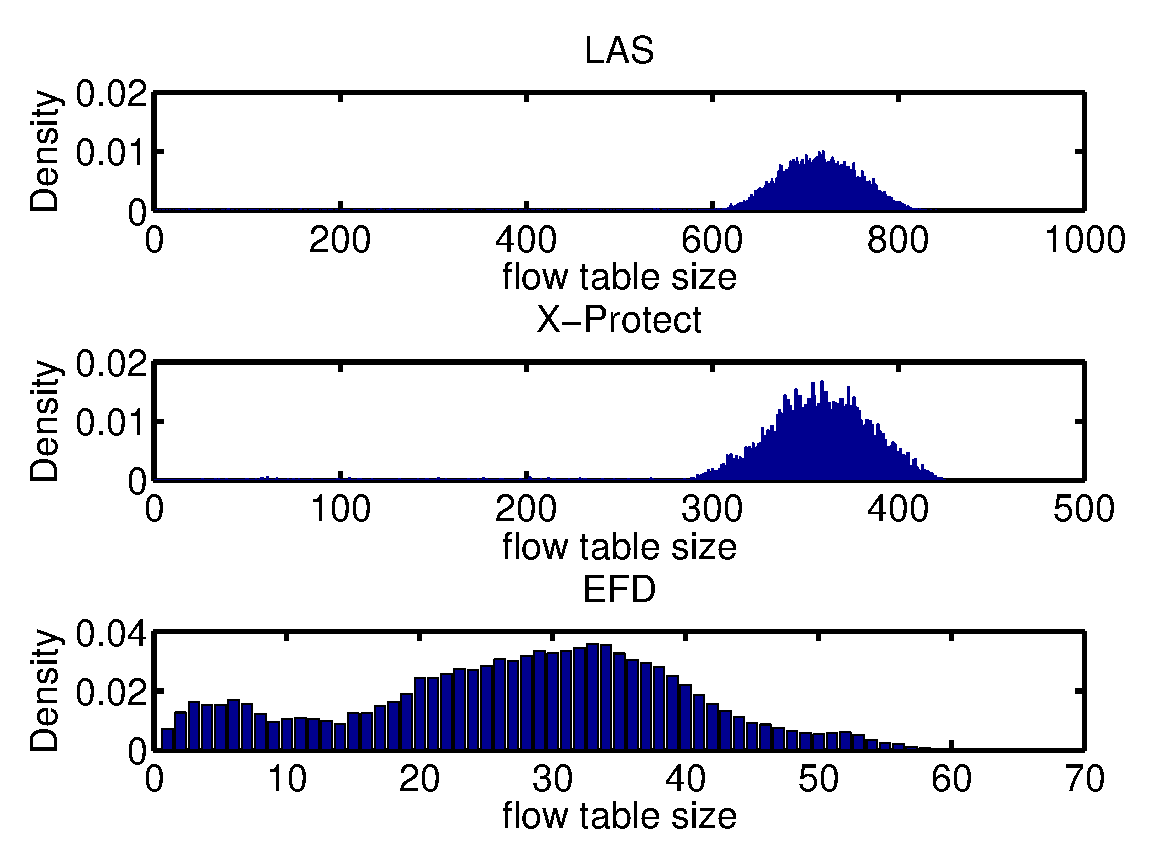
\includegraphics[width=0.49\textwidth]{./fig/wired/flow_table/density_15}}  
  \caption{Histogram of the flow table size}
  \label{fig:result12}
\end{figure}


\begin{table*}[ht]
		\centering
    \caption{Statistics - flow table size}
		\vspace{5mm}
		\resizebox{13cm}{!}{
    \begin{tabular}{ | c | c | c | c | c |}
    \hline
		\multicolumn{2}{|c|}{} & LAS & X-Protect & EFD \\ \hline \hline
		8Mbit/s & mean & 392.49 & 176.84 & 1.99 \\ \cline{2-5}
		(underload) & 95\%-CI & [392.37,  392.61] & [176.78,  176.89] & [1.9962,    2.0032] \\ \hline
		15Mbit/s & mean & 704 & 352.95 & 27.90\\ \cline{2-5}
		(overload) & 95\%-CI & [703.8,  704.2] & [352.86,  353.05] & [27.88,   27.92] \\ \hline	
    \end{tabular}
		}
    \label{tab:flow_table_size}  
\end{table*}

\subsubsection{Mean response time}

Response time is a key metric for a lot of applications, especially interactive ones. An objective of EFD and size-based scheduling policies in general  is to favor interactive applications, hence the emphasis put on response time. We consider four scheduling policies: FIFO, LAS, Run2C and EFD. FIFO is the current de facto standard and it is thus important to compare the performance of EFD to this policy. LAS can be considered as a reference in terms of (blind) size-based scheduling policies as a lot of other disciplines have positioned themselves with respect to LAS. Run2C, for instance, aims at avoiding the lock out of long flows observed more often with LAS than for \textit{e.g.}  FIFO. We do not consider the X-protect policy discussed in Section \ref{sec:table_size}, as Run2C can be considered as a perfect version of X-protect since Run2C distinguishes packets of flows below and above the threshold $\textit{th}$ (we use the same threshold $\textit{th}$ for both EFD and Run2C).

%To differentiate short flows from long flows in the figures, we adopt a simple definition: flows whose size is smaller than the 90$^\textrm{th}$ of the flow size distribution  (about 50 MSS) are considered as short flows, while the others are called long flows.

Response times are computed only for flows that complete their transfer before the end of the simulation. When comparing response times, one must thus also consider the amount of traffic due to flows that terminated their transfer and to flows that did not complete. The lack of completion of a flow can be due to a premature end of simulation. However, in overload and for long enough simulations as in our case, the main reason is that they were set aside by the scheduler. %It is thus important to analyze the distributions of the flows sizes that die not complete their transfers. 

%We first present in Figure \ref{fig:aggregate_vol} 
We first turn our attention to the aggregate volumes of traffic per policy for the underload and overload cases. We observe no significant difference between the different scheduling policies in terms both of number of complete and incomplete connections. The various scheduling policies lead to a similar level of medium\footnote{The medium is the IP path as those policies operate at the IP level.} utilization. 

%\begin{figure*}[ht!]
%  \centering
%  \subfigure[workload of 8Mbit/s (underload)]{\includegraphics[width=0.49\textwidth]{./fig/wired/incomple_8_0}}
%  \subfigure[workload of 15Mbit/s (overload)]{\includegraphics[width=0.49\textwidth]{./fig/wired/incomple_15_0}}  
%  \caption{Aggregate volumes of complete and incomplete transfers}
%  \label{fig:aggregate_vol}
%\end{figure*}

In contrast, when looking at the distribution of incomplete transfers, it appears that the flows killed by the different scheduling policies are not the same. We present in Figure \ref{fig:distrib_incomplete} the distribution of incomplete transfers where the size of a transfer is the total amount of MSS packets transferred at the end of the simulation. A transfer is deemed incomplete if we do not observe a proper TCP tear down with two FIN flags. As expected, we observe that FIFO tends to kill a lot of small flows while the other policies discriminate long flows.

\begin{figure}[ht]
  \centering
  \subfigure[workload of 8Mbit/s (underload)]{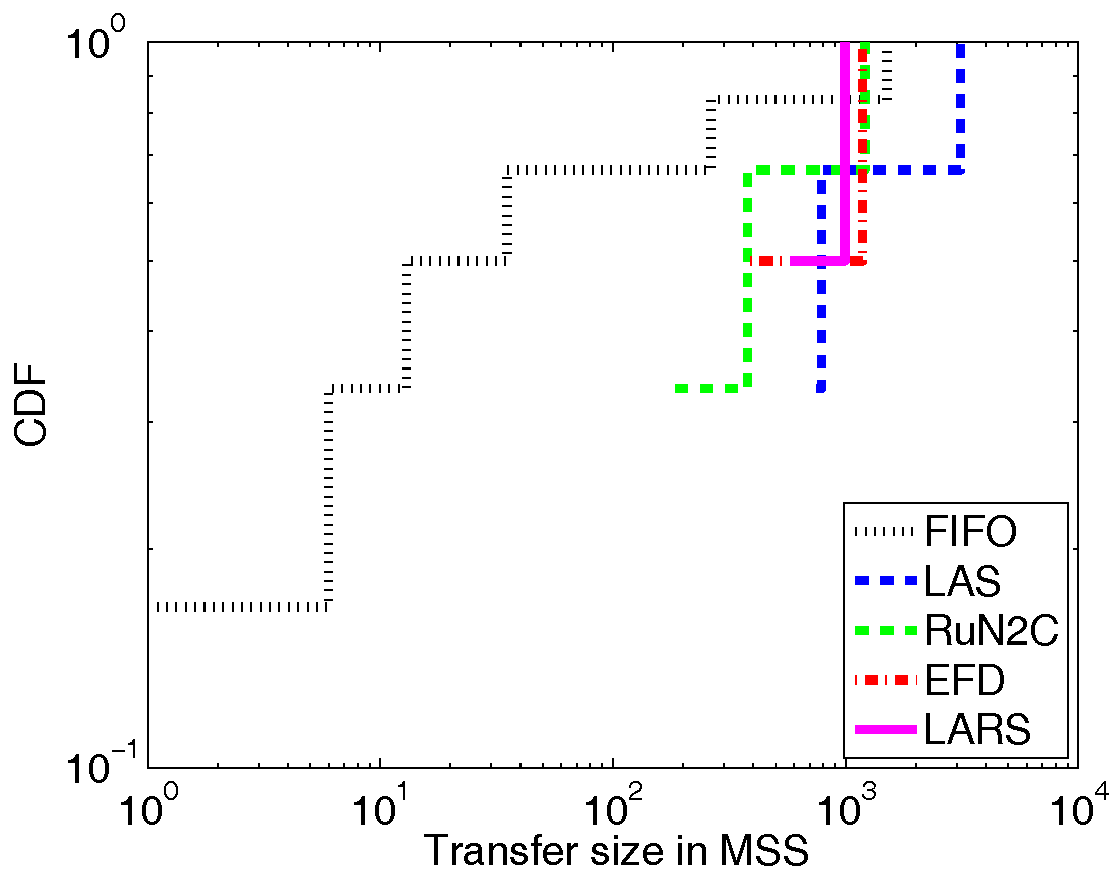
\includegraphics[width=0.49\textwidth]{./fig/wired/mean_time/cdf_incomplete_8_0}}
  \subfigure[workload of 15Mbit/s (overload)]{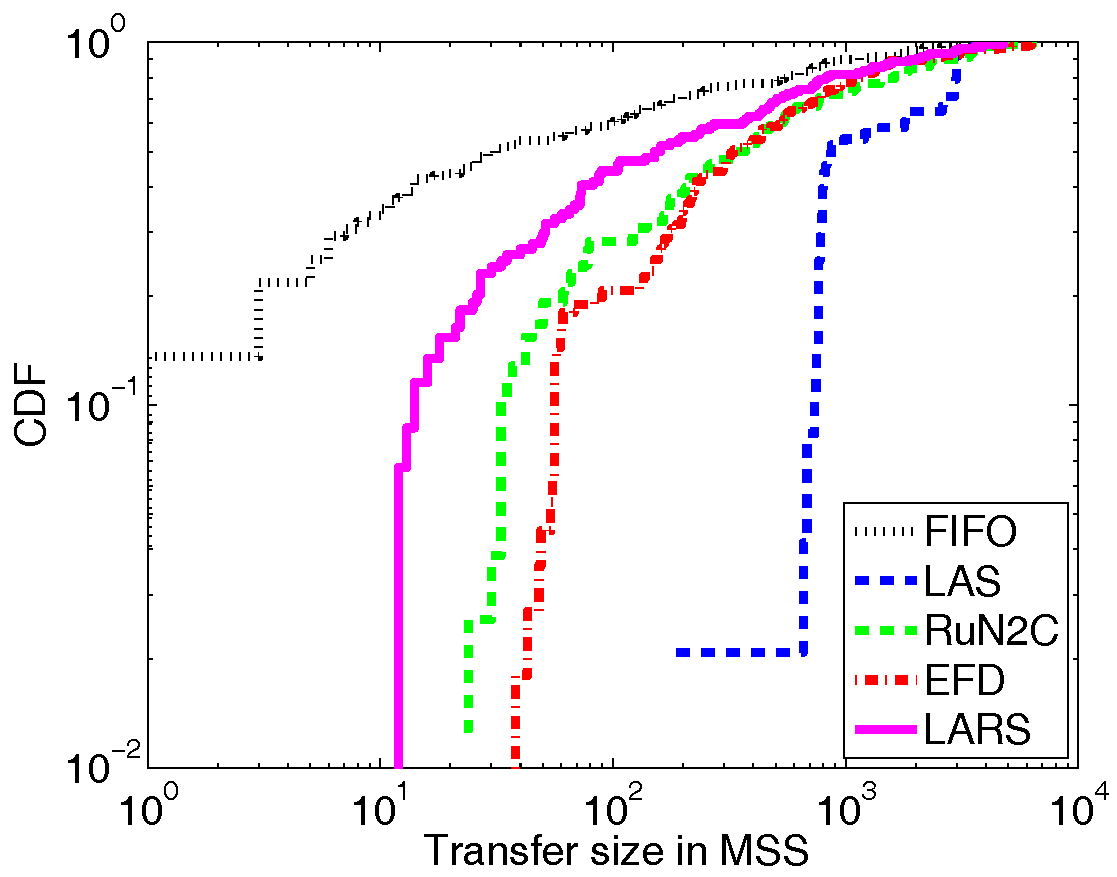
\includegraphics[width=0.49\textwidth]{./fig/wired/mean_time/cdf_incomplete_15_0}}  
  %\vspace{-5mm}
  \caption{Distributions of incomplete transfers size}
  \label{fig:distrib_incomplete}
\end{figure}


%\begin{figure*}[ht!]
%  \centering
%  \subfigure[workload of 8Mbit/s (underload)]{\includegraphics[width=0.49\textwidth]{./fig/wired/mg1_tw_fs_exp_8_0}}%{./fig/wired/boxplot_8_0}}
%  \subfigure[workload of 15Mbit/s (overload)]{\includegraphics[width=0.49\textwidth]{./fig/wired/mg1_tw_fs_exp_15_0}}%{./fig/wired/boxplot_20_0}}  
%  \caption{Conditional mean response time}
%  \label{fig:result14}
%\end{figure*}

Distributions of the response times for the (complete) short and long transfers in underload and overload conditions are presented in Figure \ref{fig:resp_time}. Under all load conditions, LAS, EFD and Run2C manage to significantly improve the response time of the short flows as compared to FIFO. EFD and Run2C offer similar performance. They both have a transition of behavior at about \textit{th} value ($\textit{th}=20$ MSS). Still, the transition of EFD is smoother than the one of Run2C. This was expected as Run2C applies a strict rule: below or above $\textit{th}$ for a given transfer, whereas EFD can further cut a long transfer into fragments which individually go first to the high priority queue. Overall, EFD provides similar or slightly better performance than Run2C with a minimal price in terms of flow bookkeeping. LAS offers the best response time of size-based scheduling policies in our experiment for small and intermediate size flows. For large flows its performance is equivalent to what other policies obtain for the underload case and significantly better for overload. However, one has to keep in mind that in overload conditions, LAS deliberately killed a large set of long flows (see Figure \ref{fig:distrib_incomplete}), hence its apparent better performance.   


%\vspace{-5mm}
\begin{figure}[ht]
  \centering
  \subfigure[workload of 8Mbit/s (underload)]{\includegraphics[width=0.49\textwidth]{./fig/wired/mean_time/mg1_tw_fs_exp_8_0}}
  \subfigure[workload of 15Mbit/s (overload)]{\includegraphics[width=0.49\textwidth]{./fig/wired/mean_time/mg1_tw_fs_exp_15_0}}  
  %\vspace{-5mm}
  \caption{Conditional mean response time}
  \label{fig:resp_time}
\end{figure}
%\vspace{-5mm}

As a complement to Figure \ref{fig:resp_time}, we plot the mean value together with the 95\% confidence interval of the response time over the flow size in Figure \ref{fig:resp_time_ci}. Remember that the distribution of flow sizes generated exhibits high variability - meaning that small number of longest flows carry the majority of traffic load. Thus, it is problematic when calculating the confidence interval of flow response time, especially for long flows as the number of long flows collected from the workload is limited. To handle this issue, we accumulate the samples by starting from a certain flow size and spanning adjacent flow sizes in an ascending order until the number of samples reaches a threshold value given (threshold value equals to 200 for example), during which the mean value of all flow sizes traversed is taken as the flow size to pair with the confidence interval. Although flow size spans a smaller range of values (up to 300 MSS) compared to Figure \ref{fig:resp_time} (up to 9000 MSS) by taking the processing method presented above, Figure \ref{fig:resp_time_ci} confirms the phenomenon observed previously. % the credibility of the simulation results. 
Also note how LARS behaves similarly to LAS in underload and degrades to fair queueing --which brings it close to FIFO in this case-- when the networks is overloaded.

%\vspace{-5mm}
\begin{figure}[ht]
  \centering
  \subfigure[workload of 8Mbit/s (underload)]{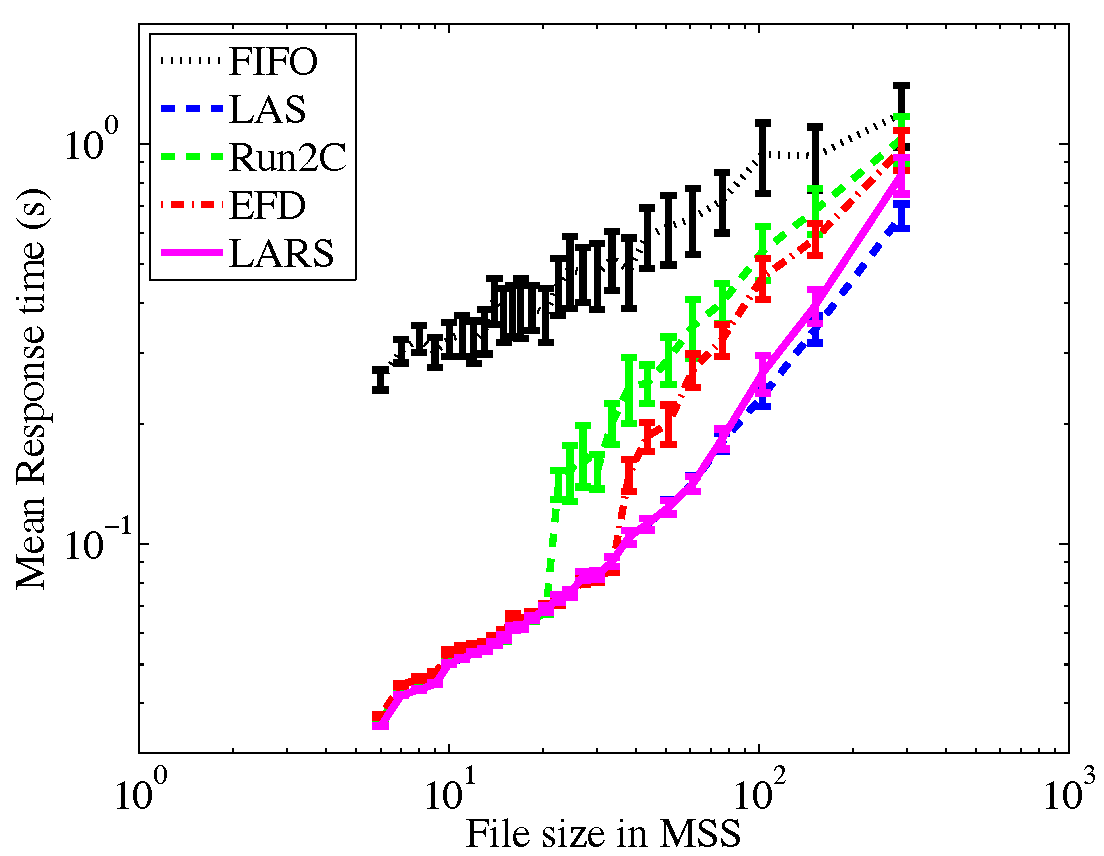
\includegraphics[width=0.49\textwidth]{./fig/wired/mean_time/CI/mg1_tw_fs_exp_8_0_log}}
  \subfigure[workload of 15Mbit/s (overload)]{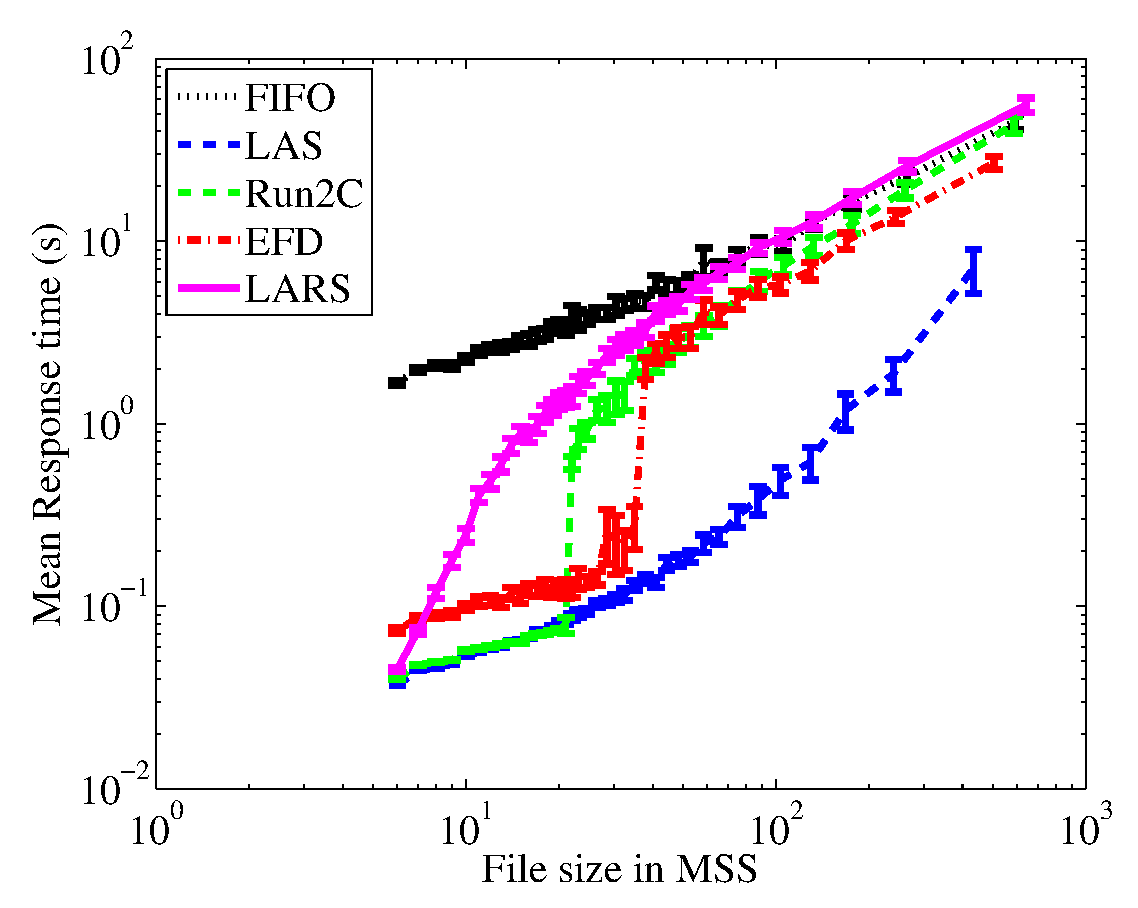
\includegraphics[width=0.49\textwidth]{./fig/wired/mean_time/CI/mg1_tw_fs_exp_15_0_log}}  
  %\vspace{-5mm}
  \caption{Confidence interval of response time over flow size}
  \label{fig:resp_time_ci}
\end{figure}
%\vspace{-5mm}


%\textcolor{red}{I know it is unpublished but shall we keep this paragraph below?}
%Given the flows which have completed their transfers before the end of the simulation - meaning that two FINs have been observed, we next partition them into short and long ones with the definition that long flows contribute to 50\% of the traffic load. This classification method coming from experimental study has the advantage that the meaning of short and long flows is consistently similar for both load regimes given in Table \ref{tab:resp_time}. We further summarize the mean value, along with the 95\% level confidence interval of data transfer response time for short and long flows respectively in Table \ref{tab:resp_time}. It makes sense as we are able to intuitively observe the improvement the new size-based scheduling brings from these statistic data in a synthetic way. Table \ref{tab:resp_time} confirms the ability of giving small response time to short flows with negligible penalty on long flows of size-based schedulings (LAS, LARS, Run2C and EFD) as compared to the legacy FIFO - in particular for the case of underload, in line with the results illustrated in Figure \ref{fig:resp_time}. 
%
%%quickly which  since the improvement are highly enphasized.   
%
%%Short and long flows are unfairly treated by size-based scheduling disciplines, it is therefore important to investigate the response time for short and long flows respectively, 
%
%\begin{table*}[ht]
%		\centering
%    \caption{Performance Statistics - 300MSS buffer - 10Mbit/s bottleneck link}
%		\vspace{5mm}
%		\resizebox{13cm}{!}{
%    \begin{tabular}{ | c | c | c | c | c | c | c |}
%    \hline
%		\multicolumn{3}{|c|}{} & \multicolumn{2}{|c|}{8Mbit/s - underload} & \multicolumn{2}{|c|}{15Mbit/s - overload} \\ \cline{4-7}
%		\multicolumn{3}{|c|}{} & short flows & long flows & short flows & long flows \\ \hline \hline
%		\multicolumn{3}{|c|}{Mean size (MSS)} & 21 & 1020 & 21 & 1086 \\ \hline
%		\multirow{10}{*}{\rotatebox{90}{Response time (seconds)}} & \multirow{5}{*}{mean} & FIFO & 0.390 & 3.519 & 3.264 & 55.788 \\ \cline{3-7}
%    & & LAS & 0.070 & 3.944 & 0.104 & 34.517 \\ \cline{3-7}
%		& & Run2C & 0.108 & 3.861 & 0.848 & 58.406 \\ \cline{3-7}
%		& & EFD & 0.090 & 3.758 & 0.705 & 40.014 \\ \cline{3-7}
%		& & LARS & 0.073 & 3.842 & 1.521 & 64.882 \\ \cline{2-7}
%		& \multirow{5}{*}{95\%-CI} & FIFO & [0.379, 0.400] & [2.709, 4.329] & [3.211, 3.317] & [48.951, 62.625] \\ \cline{3-7}
%    & & LAS & [0.069, 0.071] & [2.727, 5.161] & [0.099, 0.109] & [24.970, 44.064] \\ \cline{3-7}
%		& & Run2C & [0.104, 0.112] & [2.942, 4.779] & [0.808, 0.888] & [49.902, 66.911] \\ \cline{3-7}
%		& & EFD & [0.087, 0.093] & [2.887, 4.628] & [0.673, 0.738] & [34.397, 45.630] \\ \cline{3-7}
%		& & LARS & [0.071, 0.075] & [2.886, 4.798] & [1.471, 1.572] & [56.686, 73.078] \\ \hline	
%    \end{tabular}
%		}
%    \label{tab:resp_time}  
%\end{table*}

\subsubsection{Lock-outs}

The low priority queue of EFD is managed as a FIFO queue. As such, we expect EFD, similarly to Run2C, to avoid lock-outs observed under LAS whereby an ongoing long transfer is blocked for a significant amount of time by a newer transfer of significant size. This behavior of LAS is clearly observable in Figure \ref{fig:lockout_8_LAS} where the progress (accumulated amount of bytes sent) over time of the 3 largest transfers of one of the above simulations\footnote{Those 3 connections did not start at the same time, the time axis is relative to their starting time.}. We indeed observe large periods of times where the transfers experience no progress, which leads to several plateaus. This is clearly in contrast to the cases of LARS, EFD and to a lesser extent of Run2C, for the same connections, shown in  Figures \ref{fig:lockout_8_LARS}, \ref{fig:lockout_8_EFD} and  \ref{fig:lockout_8_Run2C}  respectively. The progress of the connections in the latter cases is indeed clearly smoother with no noticeable plateau. 

%\vspace{-5mm}
\begin{figure}[ht!]
  \centering
  \subfigure[LAS, underload\label{fig:lockout_8_LAS}]{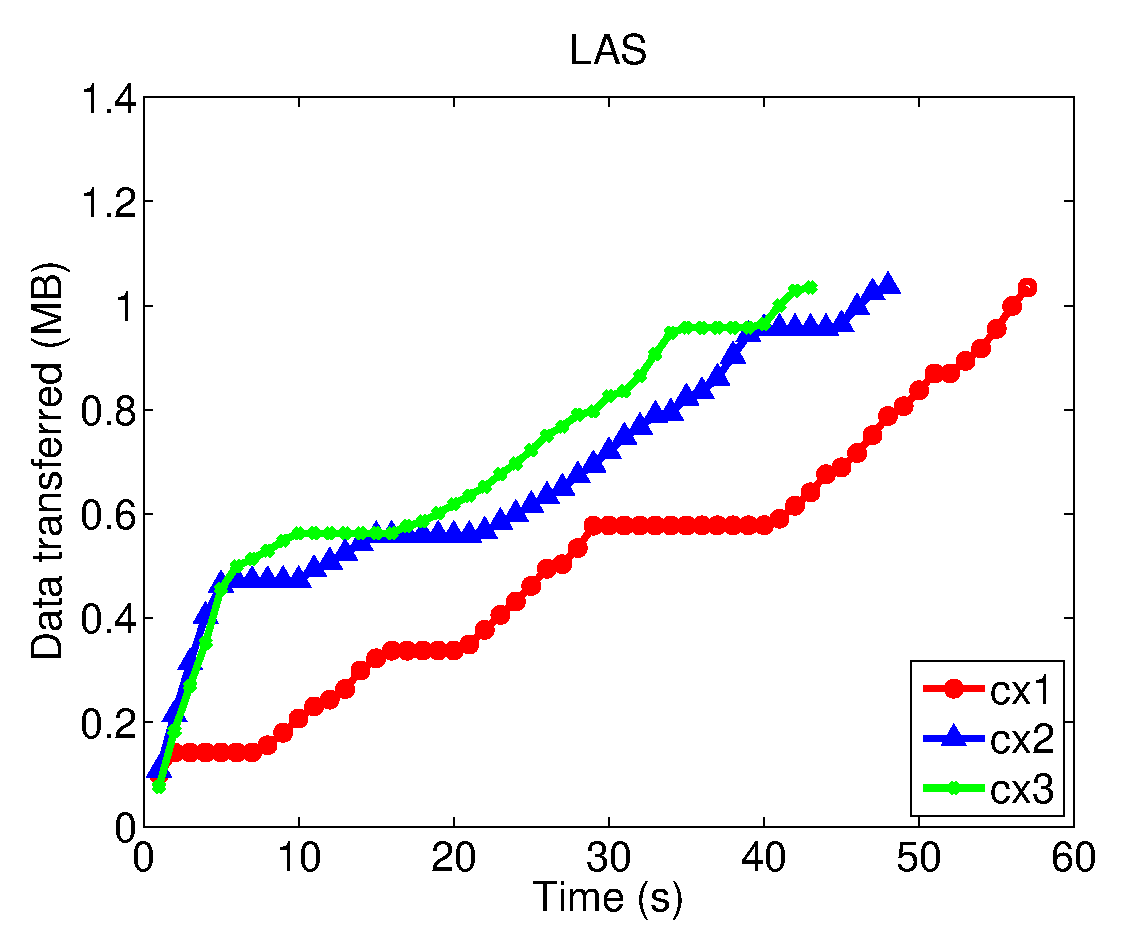
\includegraphics[width=0.49\textwidth]{./fig/wired/lock_outs/longlive_las_8}}
  \subfigure[LARS, underload\label{fig:lockout_8_LARS}]{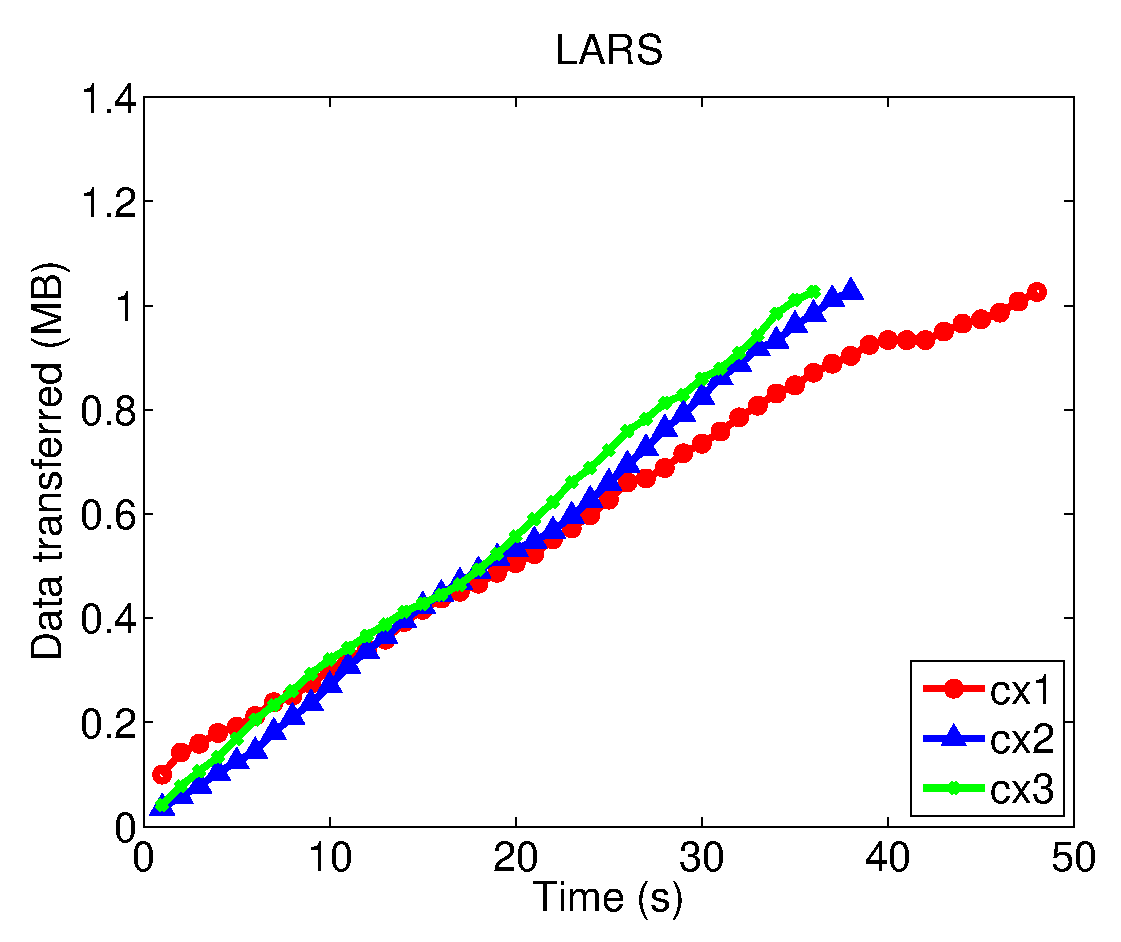
\includegraphics[width=0.49\textwidth]{./fig/wired/lock_outs/longlive_lars_8}}
  \subfigure[EFD, underload\label{fig:lockout_8_EFD}]{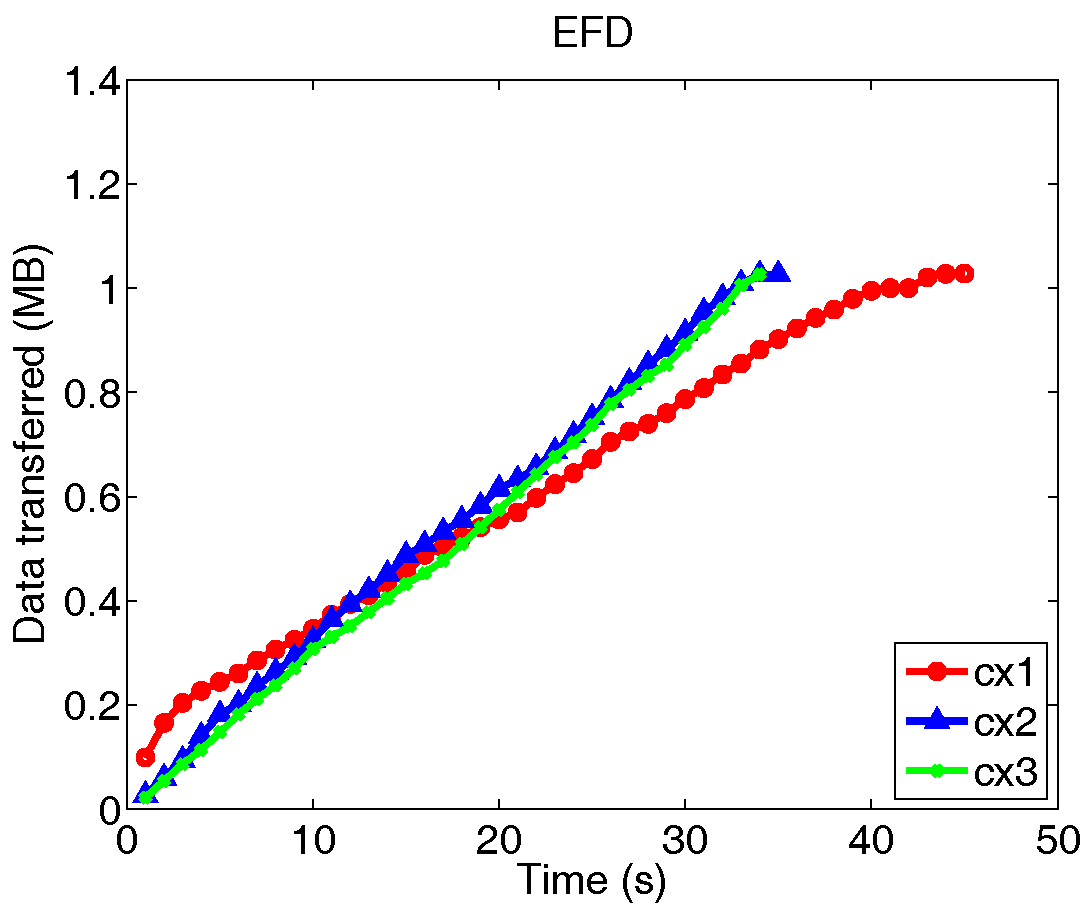
\includegraphics[width=0.49\textwidth]{./fig/wired/lock_outs/longlive_efd_8}}
  \subfigure[Run2C, underload\label{fig:lockout_8_Run2C}]{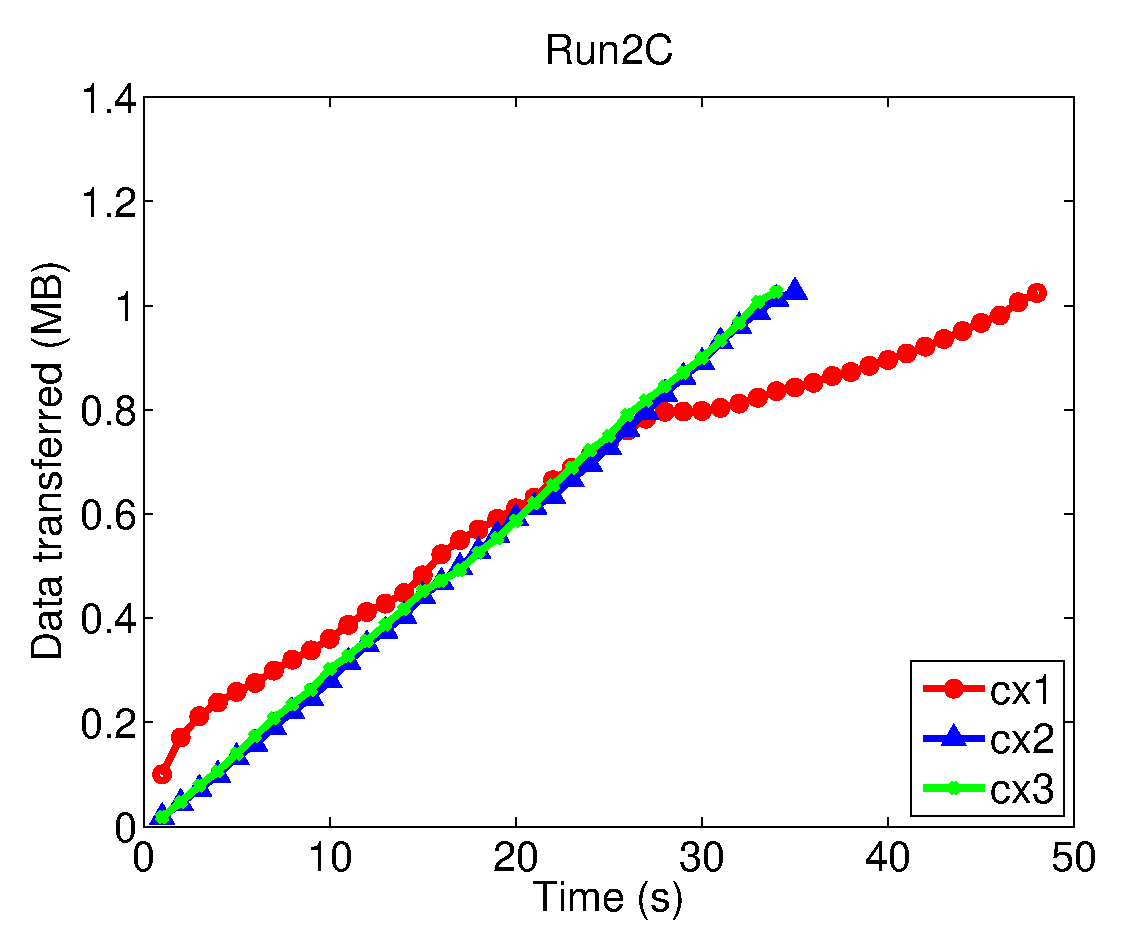
\includegraphics[width=0.49\textwidth]{./fig/wired/lock_outs/longlive_run2c_8}}
  %\vspace{-5mm}
   \caption{Time diagrams of the 3 largest TCP transfers under LAS, LARS, EFD and Run2C (underload), relative to the start of each transfer}
  \label{fig:lockout_8}
\end{figure}
%\vspace{-5mm}

%In addition, as an evidence of lock-outs, it is clear that it takes longer time for LAS to complete the long transfers as compared to EFD and Run2C, which can be easily observed from the figures.

%\textbf{Jinbang, the notations are not fully consistent between LAS and the two others (which are consitent with each other. I also wonder why cx 5 seems longer under Run2C than its equivalent under LAS and Run2C. Is there some losses at the end? In the worst case, eliminate this single connection as the rest is consistent. Though, I would prefer to know why there is this little issue....}



\subsubsection{The Case of Multimedia Traffic}\label{sec:multi_media}
In the TCP scenario considered above, FTP servers were homogeneous in the sense that they had the same access link capacity and the same latency to each client. The transfer rate was controlled by TCP. In such conditions, it is difficult to illustrate how EFD takes into accounts the actual transmission rate of data sources. In this section, we have added a single CBR flow to the TCP workload used previously.% traffic defined in Section \ref{sec:workload} (TCP transfers of Zipf distributed flow size and exponential distributed inter-arrival time). 

We consider two  rates 64Kb/s and 500Kb/s for the CBR flow, representing typical audio (\textit{e.g.}, VoIP) and video stream (\textit{e.g.}, YouTube video - even though the YouTube uses HTTP streaming)  respectively. The background load also varies - 4, 8 and 12Mbps-  which correspond to underload/moderate/overload regimes as the bottleneck capacity is 10 Mbps. To avoid the warm-up period of the background workload, the CBR flow is started at time t=10s and keeps on sending packets continuously until the end of the simulation. The simulation lasts for 1000 seconds. Since small buffers are prone to packet loss, we assign to the bottleneck a buffer of 50 packets, instead of 300 packets previously. The loss rates experienced by the CBR flow are given in Figure \ref{fig:loss_rate}, in which a well-known fair scheduling scheme called SCFQ \cite{Golestani94SCFQ} is added for the comparison, in addition to the disciplines mentioned before.

\begin{figure}[ht!]
   \centering
    %\includegraphics[width=0.55\textwidth]{./udp3/loss/udp_loss_8.eps}
  	\subfigure[a CBR flow with rate of 64Kb/s]{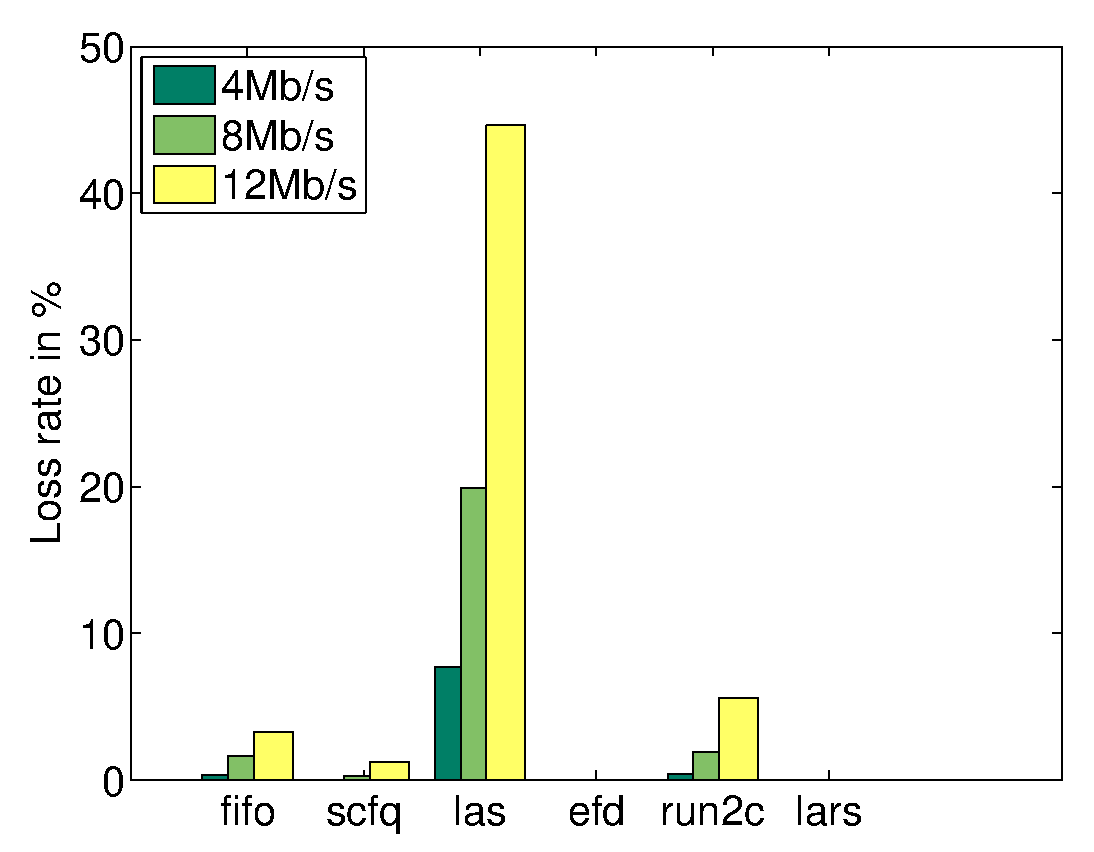
\includegraphics[width=0.49\textwidth]{./fig/wired/multimedia/loss_64/udp_loss.eps}}
  	\subfigure[a CBR flow with rate of 500Kb/s]{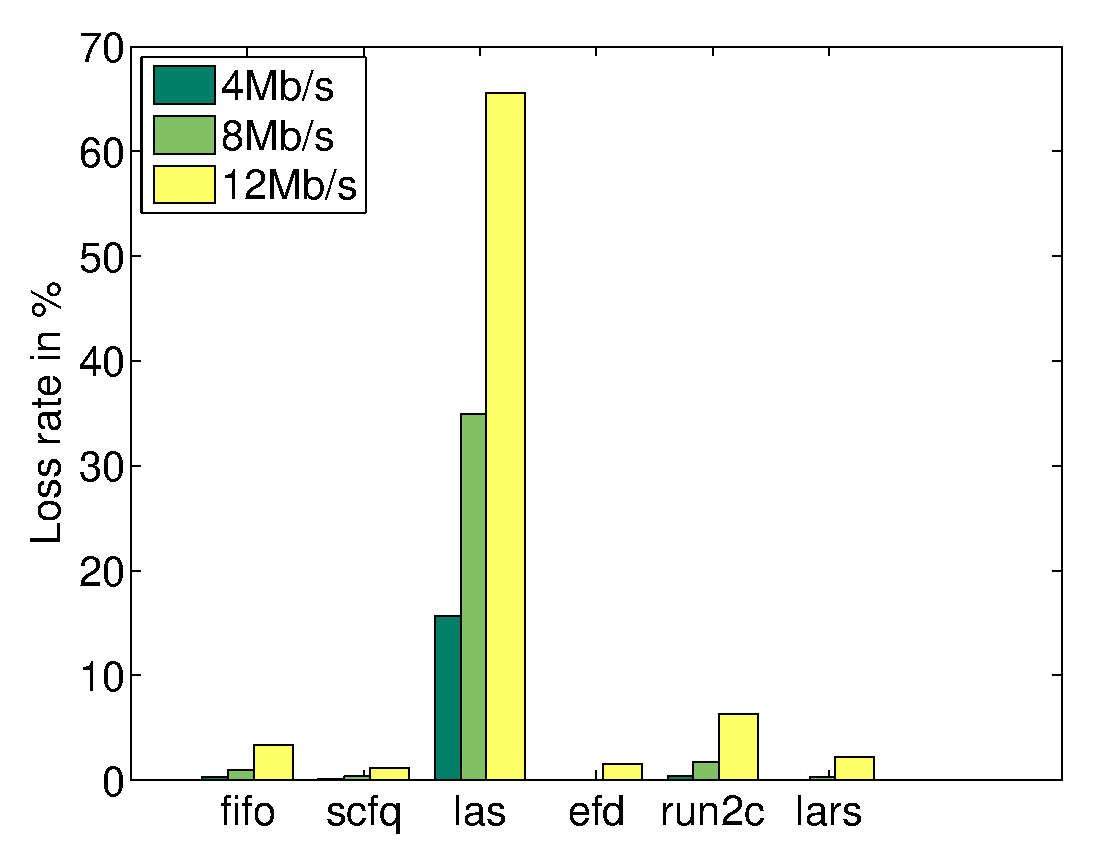
\includegraphics[width=0.49\textwidth]{./fig/wired/multimedia/loss_500/udp_loss.eps}}   
  	\caption{Loss rate experienced by a CBR flow in different background loads}
  	\label{fig:loss_rate}  
\end{figure}

As we can see from the figure, for the case of a CBR flow with rate of 64Kbps, LAS discards a large fraction of packets even at low load. This was expected as LAS only considers the accumulated volume of traffic of the flow and even at 64 kbps, the CBR flow has sent more than 8 MB of data in 1000 s (without taking the Ethernet/IP layers overhead into account). In contrast, FIFO, SCFQ and Run2C offer low loss rates in the order of a few percents at most. As for EFD and LARS, they effectively protect the CBR flow under all load conditions.

To further analyze this behavior, we next examine the inter-departure time distribution of the CBR flow \cite{Martin10Lars}. We do not report results for all three background loads but simply pick two of them  - 4Mbps and 12Mbps as they are representative for the illustration. We present them in Figure \ref{fig:jitter64} for a CBR flow with rate of 64Kbps.  We observe from Figure \ref{fig:jitter64} that, LAS serves packets in batch (many packets have short delay between them) while EFD and LARS forward packets in a much more regular way as most packets have almost the same delay between them in both background load regimes. In addition, the jitter apparently ramps up under LAS and Run2C as the background traffic grows from 4Mbps (underload) to 12Mbps (overload). 

\begin{figure}[ht]
  \centering
  \subfigure[CDF of inter-departure times for a CBR flow with 4Mb/s background traffic]{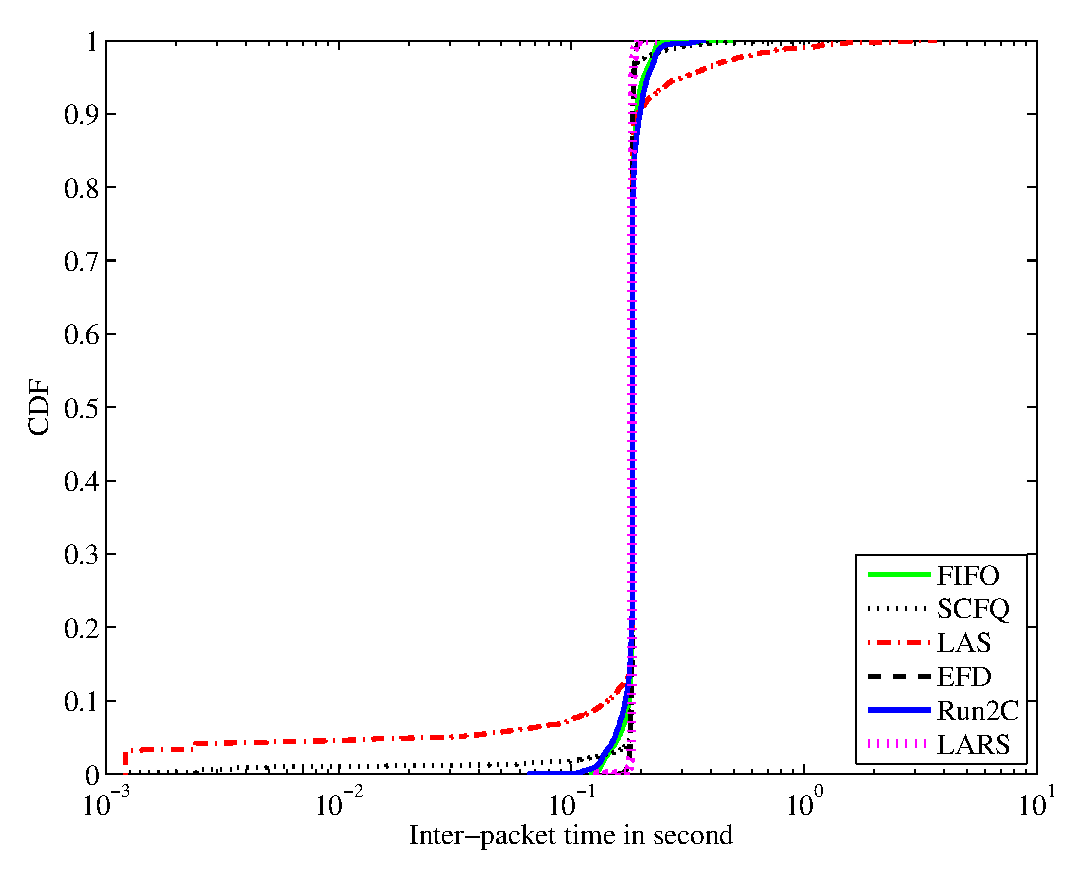
\includegraphics[width=0.49\textwidth]{./fig/wired/multimedia/jitter_64/inter_time_4.eps}}  
  \subfigure[CDF of inter-departure times for a CBR flow with 12Mb/s background traffic]{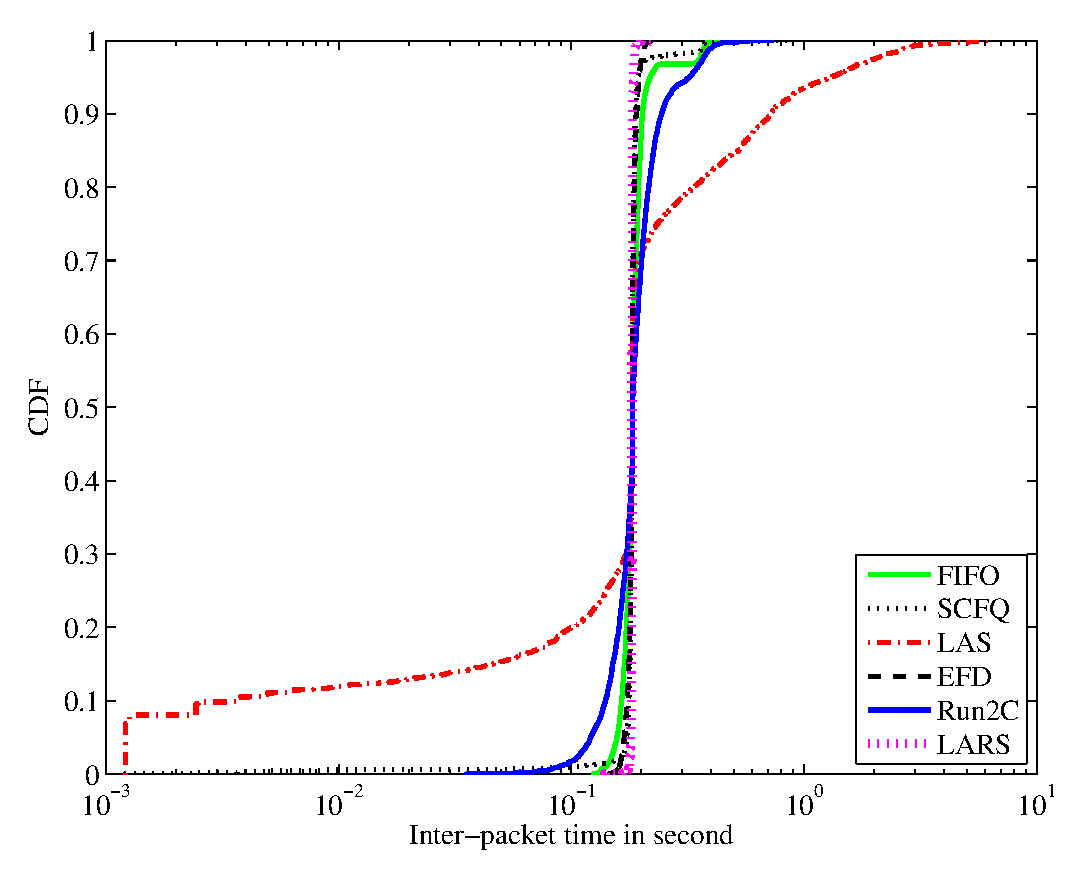
\includegraphics[width=0.49\textwidth]{./fig/wired/multimedia/jitter_64/inter_time_12.eps}}     
  \caption{Jitter of a CBR flow with rate of 64Kb/s}
  \label{fig:jitter64}
\end{figure}

%\begin{figure}[ht]
  %\centering
  %\subfigure[CDF of inter-departure times for a CBR flow with 4Mb/s background traffic]{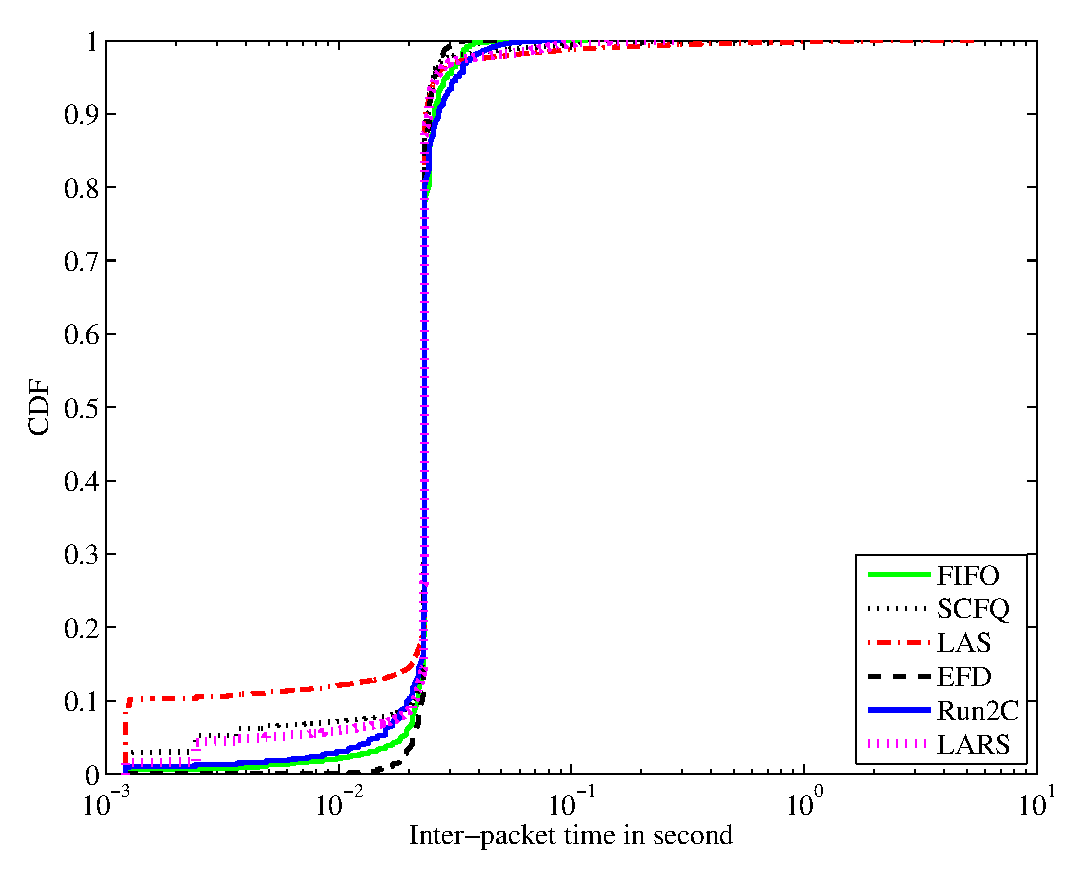
\includegraphics[width=0.49\textwidth]{./fig/wired/multimedia/jitter_500/inter_time_4.eps}}  
  %\subfigure[CDF of inter-departure times for a CBR flow with 12Mb/s background traffic]{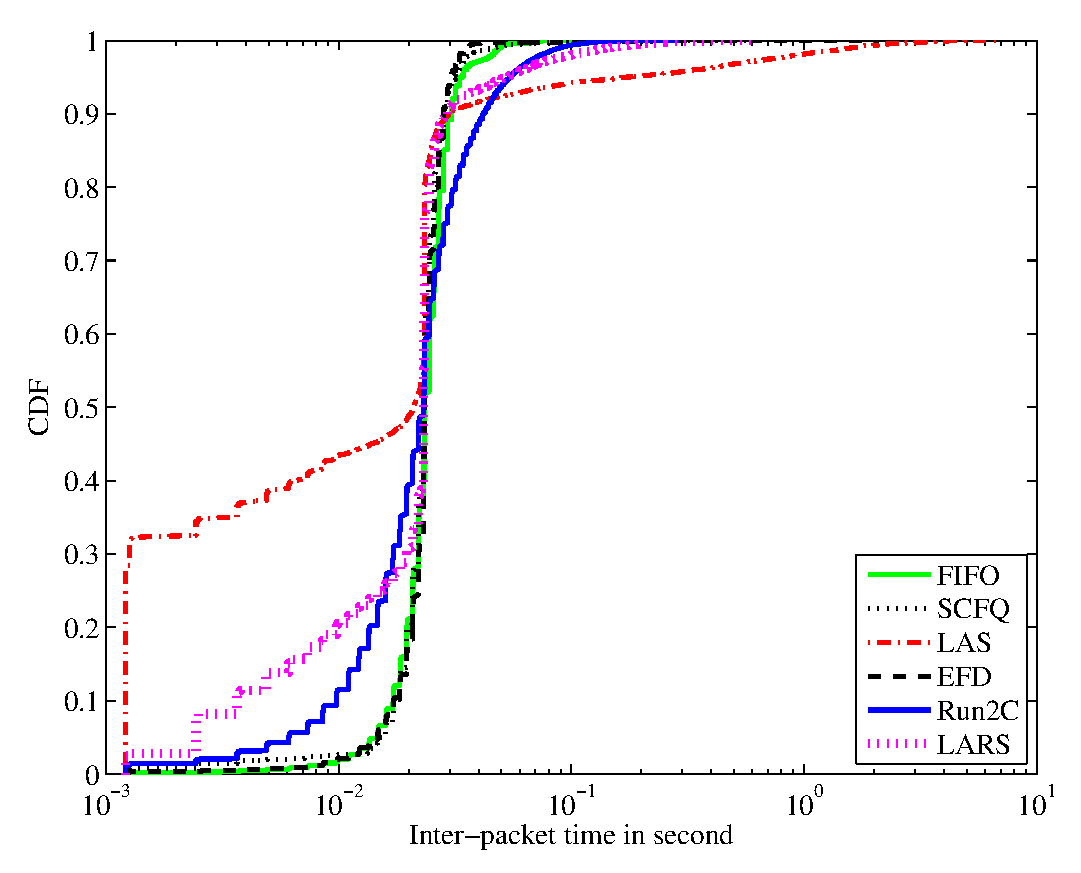
\includegraphics[width=0.49\textwidth]{./fig/wired/multimedia/jitter_500/inter_time_12.eps}}     
  %\caption{Jitter of a CBR flow with rate of 500Kb/s}
  %\label{fig:jitter500}
%\end{figure}



%\cite{Golestani94SCFQ}
As the rate of the CBR flow increases from 64Kbps to 500Kbps, no packet loss is observed for EFD in underload/moderate load  conditions, similarly to SCFQ, whereas  the other scheduling disciplines (FIFO, LAS, Run2C and LARS) are hit at  various degrees. In overload, EFD and LARS blow up similarly to LAS (which still represents an upper bound on the loss rate as the CBR flow is continuously granted the lowest priority). EFD behaves slightly better than LARS as the load in the high priority queue is by definition lower under EFD than under Run2C.%, especially the observation of packet loss under LARS. In overload regime (with the background traffic of 6Mbps), in contrast to FIFO, SCFQ and Run2C, considerable packet losses are experienced by EFD and LARS, but EFD is still better than LARS in terms of loss rate.

When looking at the above results from a high level perspective, one can think at first sight that FIFO and SCFQ do a decent job as they provide low loss rates to the CBR flow in most scenarios (under or overload). However, those apparently appealing results are a side effect of a well-known and non desirable behavior of FIFO. Indeed, under FIFO, the non responsive CBR flow adversely impacts the TCP workload, leading to high loss rates. This is especially true for the CBR flow working at 500 kbps. SCFQ tends to behave similarly if  not paired with an appropriate buffer management policy \cite{Golestani94SCFQ}. In contrast, LARS and EFD offer a nice trade-off as they manage to simultaneously grant  low loss rates to the CBR flow with a low penalty to the TCP background workload. Run2C avoids the  infinite memory of LAS but still features quite high loss rates since the CBR flow remains continuously stuck in the low priority queue.


Overall, EFD manages to keep the desirable properties of size-based scheduling policies and in addition manages, with a low bookkeeping cost, to protect multimedia flows as it  implicitly accounts for the rate of this flow and not only its accumulated volume. 


\section{EFD over a half-duplex link}
\label{sec:perf_wlan}
%EFD is designated with quite large buffers of typically 300 packets in mind, which is not unusual for routers. 
In this section, we evaluate the performance of EFD's adaptations, EFDACK and PEFD,  to  802.11  networks. % , where buffer sizes tend to be smaller as they typically range between 30 and 100 packets. 
We consider  typical infrastructure-based WLAN, esp. enterprise networks, where the Access Point (AP) constitutes the performance bottleneck. Another challenge for PEFD and EFDACK stems from the half duplex nature of  the legacy DCF method, which %,  the AP relays traffic to and from the wired network. In many cases,  the wireless LAN is the performance bottleneck, \textit{e.g.}  companies or labs frequently use access links to the Internet with 100 Mbit/s or higher  capacity. 
leads to the so called ``TCP Unfairness'' \cite{Pilosof03understandingtcp} problem -- where uploads from wireless stations get a higher fraction of the shared channel capacity than downloads. 

PEFD and EFDACK are implemented at the IP layer, leaving the MAC layer unchanged.  A last challenge for EFD in WLAN is the smaller amount of memory available at the AP, which directly constrains the memory of the scheduler. Indeed, typical APs feature shared memory chips able to buffer between 30 and 100 packets.
%Recently, several size-based scheduling solutions proposed to improve the performance of short transfers \cite{Rai2004Performance,Avrachenkov04Run2c}, have been analyzed to solve the TCP unfairness problem, \textit{e.g}, LASACK \cite{Keller2008Improving} and LARS \cite{heusse2011least}. As a variant of LAS for a half-duplex symmetric bandwidth scenario (\textit{e.g.} , 802.11 WLAN), LASACK bases its decision on the total amount of bytes sent so far by each flow in both directions by looking up the ACK number in the TCP header. LARS capitalizes on the same idea as LASACK to handle bi-directional flows over half-duplex links, and at the same time applies a temporal decay to the service obtained by a flow, which helps to bound the impact of a new flow on ongoing ones and incorporate the flow rate as a factor on the scheduling decision, as well as the volumes. In this section, we evaluate the performance of EFDACK and PEFD, and compare them to state-of-the-art size-based scheduling policies, Run2C, LASACK, LARS and also FIFO and SCFQ. 

\subsection{Evaluation methodology} \label{sec:wireless_methodology}

%In this section, we provide a high level overview of the evaluation methodology we apply to compare the variants of EFD to state-of-the-art scheduling policies. 

%\subsubsection{Network Configuration}
In our simulations for 802.11 wireless networks, we consider a simple network configuration, in which ten wireless stations communicate with ten servers in the wired part of the network across an access point, as depicted in Figure \ref{fig:setup}. We use the 802.11a protocol with nominal bit rate of 54Mb/s, with RTS/CTS disabled. Good and fair radio transmission conditions are guaranteed as the ten wireless stations are at the same physical distance (within 10 m) from the access point and in line of sight of each other. The ten wired hosts are connected to a router with an output rate 10 times larger than its input rate, so that its output queue never builds up. With such a configuration, the bottleneck if any, is the access point. We use QualNet 4.5 to obtain all simulation results.  TCP NewReno is used with delayed ACK enabled in the simulations. 


\begin{figure}[!ht]
   \centering
    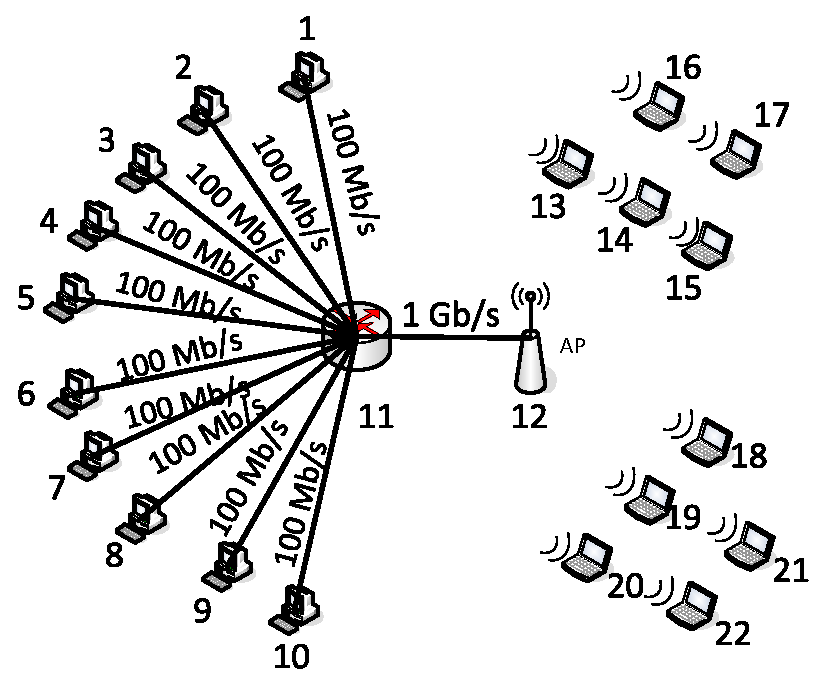
\includegraphics[width=0.5 \textwidth]{./fig/wireless/setup/wlan_topology_bandwidth.eps}
  \caption{Network Set-up, with one way delay of 2ms in wired part}
  \label{fig:setup}  
\end{figure}

\subsubsection{Workload Generation}
%We consider essentially two workloads. First, we use only long-lived flows: while unrealistic, results obtained under such a workload enable to pinpoint easily some fundamental characteristics of a scheduling policy, due to the relative simplicity of the scenario. 

To evaluate the performance of EFD and its variants in 802.11 WLANs, we have considered a realistic synthetic workload with a mix of short and long TCP transfers. We assume that TCP connections use 1460 bytes MSS and arrive according to a Poisson process with rate $\lambda$. We have adjusted $\lambda$ to obtain two load regimes: 10 Mb/s (moderate load) and 20 Mb/s (high load). For reference, a single TCP transfer can achieve a maximum throughput of 27.3 Mb/s over 802.11a at 54 Mb/s \cite{Matthew2003}. TCP transfers'  size is drawn from a bounded Zipf distribution with an average size of about 60 Kbytes (40 packets with size of 1500 bytes each), which is in line with the measurements performed on typical large WLANs \cite{MengWYL04}. The minimum transfer size is 6 MSS, and the maximum transfer volume corresponds to 10 MB with a coefficient of variation\footnote{The CoV is defined as the ratio of the standard deviation to the mean of a distribution. The larger it is, the more skewed the distribution. } of about 6, which controls how  mass is split between short and long transfers. %Note that bounded Zipf is a discrete equivalent of a continuous (bounded) Pareto distribution, and Pareto is a long tailed distribution usually adopted for modeling flows in the Internet. 
%Each packet has a fixed size of 1500 bytes in our simulations. 

A last important parameter of the workload in a 802.11 scenario, is the ratio between download and upload traffic. We denote by $\lambda_{d}$ and $\lambda_{u}$ the arrival rate of TCP downloads and uploads respectively. We considered initially  three scenarios: $\frac{\lambda{d}}{\lambda{u}}$=1 for symmetric load, $\frac{\lambda{d}}{\lambda{u}}$=10 and $\frac{\lambda{d}}{\lambda{u}}$=100 for two asymmetric loads respectively. Those three scenarios are related to real use cases. The case $\frac{\lambda{d}}{\lambda{u}}$=10  corresponds to a typical residential user browsing the Web with no  heavy P2P nor HTTP streaming (YouTube, DailyMotion, \textit{etc.}) activity \cite{Pietrzyk2011}. Clients that rely heavily on P2P tend to produce more symmetric ratios, corresponding to $\frac{\lambda{d}}{\lambda{u}}$=1. On the other side of the spectrum, a trend in residential network is to see more and more heavy hitters characterized by a heavy HTTP streaming activity \cite{Pietrzyk2011}. In such a scenario, almost all bytes flow from the server to the client, leading to ratios close to 100.


To gain insights about the typical traffic within an enterprise network, we captured one full day of traffic within the Eurecom network - a medium size research lab%\footnote{In the context of the ELAN projet \url{http://elan.eurecom.fr/}}
, which comprises about 600 machines and 60 servers. We analyzed the ratio of download to upload traffic for intranet traffic and Internet traffic of each host and found that Internet traffic corresponds to an average ratio of 10, as users mostly browse the Internet, without heavy HTTP streaming activity. In contrast, intranet traffic (SMB, LDAP, \textit{etc}.) is  larger in volume and highly symmetric, \textit{i.e.} characterized by ratio close to 1. A reason why the ratio of the latter is symmetric is that P2P traffic is banned from the network, as from most enterprise networks in general. 


Hereafter, we consider the cases  $\frac{\lambda{d}}{\lambda{u}}$=1 for symmetric load, and $\frac{\lambda{d}}{\lambda{u}}$=10 for asymmetric load as the case $\frac{\lambda{d}}{\lambda{u}}$=100 is less frequent in enterprise networks and degenerates to the pure download case, where the TCP unfairness problem typically vanishes. %We sum up the simulation parameters in Table \ref{tab:simu_para}.


%\begin{table}[tch]
%		\centering
%		\caption{Simulation parameters for the evaluation in 802.11 WLANs}		
%		\vspace{5mm}
%		\resizebox{10cm}{!}{
%		\begin{tabular}{ | c | c | c | c | }
%		\hline
%		\multicolumn{2}{|c|}{Simulator} & \multicolumn{2}{|c|}{QualNet 4.5} \\ \hline
%		\multicolumn{2}{|c|}{MAC protocol} & \multicolumn{2}{|c|}{802.11a@54Mbit/s} \\ \hline \hline
%		\multirow{6}{*}{\rotatebox{90}{Workload}} & buffer size & \multicolumn{2}{|c|}{30MSS / 300 MSS} \\ \cline{2-4}
%		& transfer size distr. & \multicolumn{2}{|c|}{bounded Zipf} \\ \cline{2-4}
%		& \multirow{2}{*}{load regimes} & medium & 10 Mbit/s \\ \cline{3-4}
%		& & high & 20 Mbit/s \\ \cline{2-4}
%		& \multirow{2}{*}{traffic ratio} & sym. & $\lambda_{d}/\lambda_{u} = 1$ \\ \cline{3-4}
%		& & asym. & $\lambda_{d}/\lambda_{u} = 10$ \\ \hline		
%		\end{tabular}
%		}
%		\label{tab:simu_para}  
%\end{table}
%
%\vspace{-5mm}

%\subsubsection{Performance Metrics}

%We focus on two performance metrics in our study. First, the global volumes uploaded and downloaded. It is important to keep an eye on this metric to assess the ability of a scheduling policy to effectively use the available network capacity. Secondly, the conditional response times in each flow direction as they allow to observe how the scheduling discipline treats each flow size and also if unfairness exists between uploads and downloads or between flows of various sizes. 


%\subsection{The discussion of the AP buffer units} \label{sec:buffer_granularity}
%In 802.11 scenario, before assessing the performance of EFD policy in depth, we first discuss the effect of the AP buffer granularity. We term the buffer granularity as the unit in which the buffer size of the network device interface is measured, and we use two units for that in our discussion - byte and packet, although networking devices generally limit the size of their queues by the number of packets they can hold as opposed to the number of bytes the packets are worth.%, although some devices indicate the memory in bytes by default by the manufacturer. %In addition, we restrict our discussion to 802.11 Wireless LANs, in which the unfairness issue is commonly raised and highlighten\cite{Pilosof03understandingtcp}. 
%
%Let us consider a scenario of five upload and five download long-lived connections, with the ratio of download to upload traffic equal to 1. To show the possible effect that different buffer units may bring, we simply discuss how the FIFO discipline reacts to the varying units of the AP buffer size - which typically ranges between 30 and 100 packets. When the buffer size is measured in packets - meaning that the buffer is configured to be filled packet by packet, and the buffer full-checking is performed with the unit of number of packets - five upstream flows will easily fill up the buffer by emitting at most $5\times(43/2)$ ACKs simultaneously (with delayed ACK enabled and the receiver's advertised window of 65 KB - equivalent to 43 MSS). In contrast, significant space will be left for data packets of downloads to grab for the case where the buffer size is measured in bytes since $5\times(43/2)$ ACKs with size of 40 bytes each make up only a small percentage of the buffer (For example, with the maximum buffer size of 30 MSS, $5\times(43/2)\times40$bytes which comes to 4.3KB account for less than 10\% of the buffer size). Consequently, more packets of downloads are able to be incorporated in the buffer and avoid being dropped. 
%
%In this part, we restrict ourselves to the discussion on the impact of the buffer granularity on TCP performance of scheduling policies in 802.11 networks, in which data typically flows in both directions. For simplicity, we consider initially the symmetric load, \textit{i.e.} $\frac{\lambda_{d}}{\lambda_{u}} = 1$. The disciplines to be discussed include LASACK, LARS, Run2C, BEFD, PEFD, EFDACK, as well as FIFO and SCFQ. As in 802.11 scenario in the case of Run2C \cite{Avrachenkov04Run2c}, we use a variant that takes into account the volume transferred in both directions (by tracking ACK number progress). We refer to it as Run2CACK. 
%
%%Since TCP accounts for more than 90\% of the Internet traffic, a TCP centric approach to measure the impact of buffer granularity would be appropriate in practice. We consider TCP traffic only and report the results for TCP connections. When conducting simulations for scheduling disciplines, it is interesting to highlight the impact of having a buffer in bytes or in packets granularity for unidirectional and bidirectional traffic. We restrict ourselves to the case of single bottleneck link. The simulation methodology is similar to the one presented in Section \ref{sec:wireless_methodology}. 
%
%We investigate the impact of buffer granularity by examining the conditional response time of uploads and downloads, assuming a highly skewed (as the coefficient of variation is 6) flow size distribution. We run the simulations for a moderate load of 10Mbit/s, setting the buffer size to be 30 MSS. The simulations are conducted  in two scenarios with different buffer granularity - the unit of packets and bytes respectively. Each simulation lasts 1000 seconds. We demonstrate the results in Figure \ref{fig:realistic_one} and Figure \ref{fig:realistic_two}, in which line styles along with colors are used to denote different scenarios (with unit of byte or packet), whereas line widths are used to indicate traffic in two directions. 
%
%\begin{figure*}[ht!]
%  \centering
%  \subfigure[FIFO]{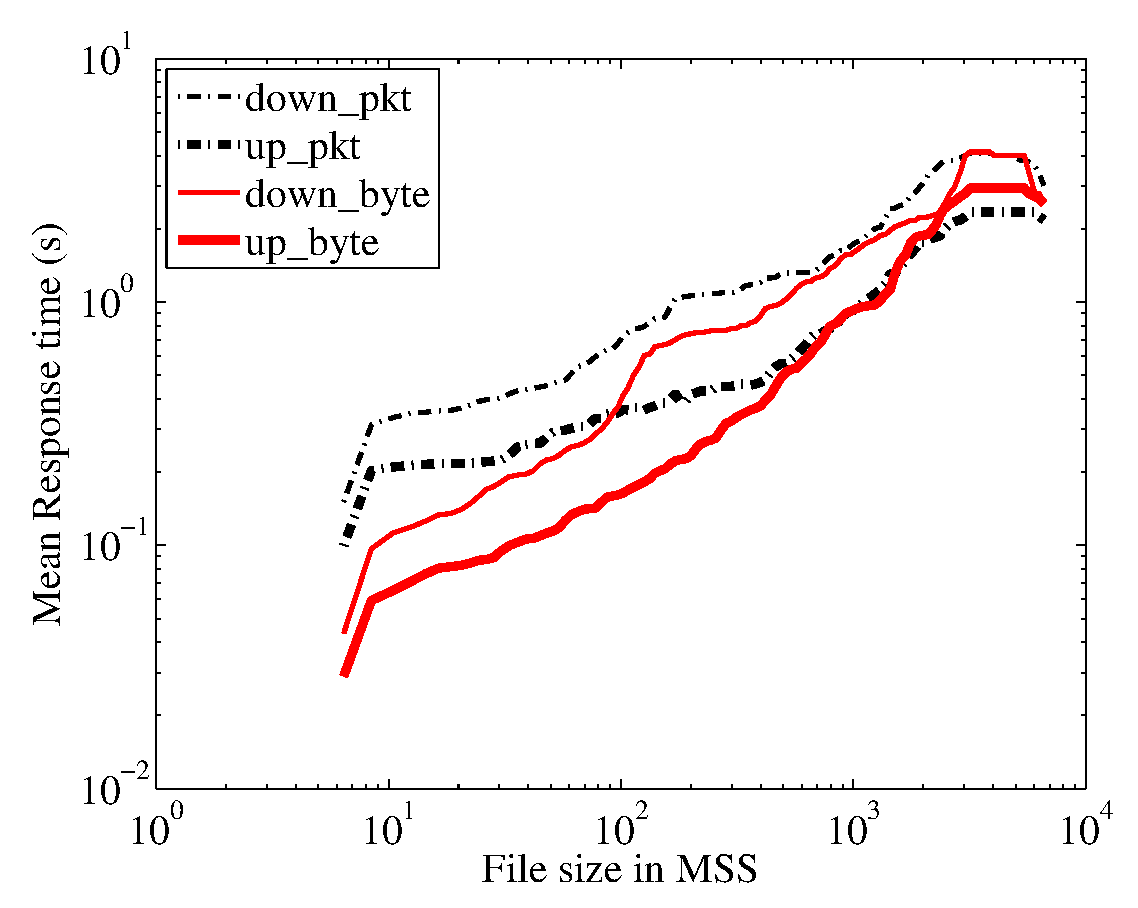
\includegraphics[width=0.495\textwidth]{./fig/buffer/realistic/mg1_mixed_fifo_10_0.eps}}
%  \subfigure[SCFQ]{\includegraphics[width=0.495\textwidth]{./fig/buffer/realistic/mg1_mixed_scfq_10_0.eps}}
%  \subfigure[BEFD]{\includegraphics[width=0.495\textwidth]{./fig/buffer/realistic/mg1_mixed_befd_10_0.eps}}		
%	\subfigure[Run2CACK]{\includegraphics[width=0.495\textwidth]{./fig/buffer/realistic/mg1_mixed_llasn_10_0.eps}}			
%  \caption{Average response time, symmetric load, 10Mbit/s workload}
%  \label{fig:realistic_one}
%\end{figure*}
%
%\begin{figure*}[ht!]
%  \centering
%  \subfigure[LASACK]{\includegraphics[width=0.495\textwidth]{./fig/buffer/realistic/mg1_mixed_lasack_10_0.eps}}
%  \subfigure[LARS]{\includegraphics[width=0.495\textwidth]{./fig/buffer/realistic/mg1_mixed_lars_10_0.eps}}
%  \subfigure[PEFD]{\includegraphics[width=0.495\textwidth]{./fig/buffer/realistic/mg1_mixed_pefd_10_0.eps}}
%  \subfigure[EFDACK]{\includegraphics[width=0.495\textwidth]{./fig/buffer/realistic/mg1_mixed_efdack_10_0.eps}}	
%  \caption{Average response time, symmetric load, 10Mbit/s workload (cont.)}
%  \label{fig:realistic_two}
%\end{figure*}
%
%In the case of mixed workload - which is believed to be close to the reality, measuring the buffer with the unit of bytes is highly preferred for FIFO, Run2CACK and BEFD as it provides significantly lower conditional response time for the majority of the flows in both two directions, especially for small and medium size flows, although the unfairness between uploads and downloads in terms of response time exists and is not improved by the observation from Figure \ref{fig:realistic_one}. Recall that the unfairness in 802.11 WLANs lies in the competition for accessing the limited buffer of the AP between the upload and the download. When the buffer size is in bytes, the download is granted more opportunities to reside in the queue and then to be served, avoiding being dropped frequently as what happens in the scenario of packet-based buffer granularity. 
%
%%which is quite similar to the case of long-lived connections - although different metrics are used to measure the performance in two workload cases. 
%
%
%Not surprisingly, SCFQ, LASACK, LARS, PEFD, EFDACK are observed to be insensitive to the buffer granularity in the case of mixed workload with heavy-tailed flow size distribution. However, the unfairness is quite pronounced for SCFQ, in terms of high performance discrepancy between uploads and downloads. Unlike SCFQ, the other policies (LASACK, LARS, PEFD, EFDACK) shown in Figure \ref{fig:realistic_two} enforce a good level of fairness for most of the flow sizes. 
%
%In summary, we investigate the impact of the buffer granulartiy (instead of the buffer sizing) on the performance of scheduling disciplines over 802.11 WLANs in this part. The discussion is conducted with two buffer granularities - packets and bytes. We investigate the mean conditional response time in the case of realistic synthetic workload with heavy-tailed size distribution. We conclude that measuring the buffer with the unit of bytes is highly preferred for FIFO, Run2CACK and BEFD, while LASACK, LARS and SCFQ are insensitive to the buffer granularity. 
%
%One of the lessons of the above discussion is that, SCFQ and BEFD are clearly ineffective when the traffic consists of both uploads and downloads. This is why we rule them out from further investigation bellow. One can argue that this is also the case for FIFO. However, as FIFO is the legacy scheduling discipline, we keep it as a reference point hereafter.

\subsection{Realistic synthetic workload} \label{section:realistic_workload}
In this part, we first investigate the impact of varying the scheduling discipline for EFD-like schemes. We consider 4 combinations of disciplines: FIFO+FIFO, LAS+FIFO, FIFO+LAS, LAS+LAS  in two different flavors corresponding to  a threshold either in byte like in EFDACK or in  packets like PEFD. We conclude that the original FIFO+FIFO is a good candidate and thus focus only on the original PEFD and EFDACK in subsequent analysis.

We next compare PEFD and EFDACK to FIFO, LARS, LASACK and Run2CACK.  We examine the conditional response time of uploads and downloads, assuming a highly skewed (as the coefficient of variation is 6) flow size distribution.  Finally, we discuss the impact of the buffer size at the AP on the performance of scheduling policies in 802.11 networks. 

To highlight the benefits of size-based scheduling policies compared to FIFO, we have configured the AP buffer size to be measured in packets. We use two buffer sizes - 30 MSS and 300 MSS - to represent respectively small and large buffer size. Each simulation lasts for 5000s. %Some connections are unfinished at the end of a simulation due to the premature end of simulation; however, under high load and for long enough simulations as in our case, the main reason is that they were set aside by the scheduler. 
We report performance results only for the connections that have completed a transfer. We do not represent on the figures the confidence intervals  (for each flow size) as, given the number of curves per figure, they tend to obscure the graphs. Still, they enabled us to check that the simulations were long enough to draw conclusions based on the conditional mean response times. 

\subsubsection{Comparison of EFD Variants} \label{section:4schemes}

In this part, we consider four variants of EFD: LAS+FIFO, FIFO+LAS, LAS+LAS as well as FIFO+FIFO itself. For each variant, we have two flavors, depending on the bookkeeping option which is either in bytes like EFDACK or packets as PEFD.%Our results in previous sections demonstrate that the two options we considered to adapt EFD to WLAN, namely counting volumes in packets or counting in bytes but considering the sequence numbers of TCP ACK are viable options. We thus consider those two strategies for each of the 4 scheduling policies here. 

Before going into the details, we need to explicit the way LAS is used here. This is the global EFD scheduler that assigns the volumes, either in packets or bytes depending on the strategy. Each packet is thus marked with an associated volume and, when LAS is used, it manages the queue where it is applied in such a way that packets are always sorted in ascending order of their associated volume.

We conducted experiments with a symmetric load and 10 Mb/s (moderate load) and 20 Mb/s (high load) respectively. The buffer size is set to 30 packets. Average conditional response times of byte-based schemes are depicted in Figure \ref{fig:asym_byte} while the case for the packet-based schemes are illustrated in Figure \ref{fig:asym_pkt}. Results with an asymmetric load are qualitatively similar and we do not present them here.

\begin{figure*}[ht!]
  \centering
  \subfigure[Workload of 10Mbit/s]{\includegraphics[width=0.495\textwidth]{./fig/wireless/4schemes/byte/mg1_tw_fs_exp_10_0.eps}}
  \subfigure[Workload of 20Mbit/s]{\includegraphics[width=0.495\textwidth]{./fig/wireless/4schemes/byte/mg1_tw_fs_exp_20_0.eps}}  
  \caption{Comparison between various queueing policies in EFD  queues -- Average response time, symmetric load, byte-based}
  \label{fig:asym_byte}
\end{figure*}

\begin{figure*}[ht!]
  \centering
  \subfigure[Workload of 10Mbit/s]{\includegraphics[width=0.495\textwidth]{./fig/wireless/4schemes/pkt/mg1_tw_fs_exp_10_0.eps}}
  \subfigure[Workload of 20Mbit/s]{\includegraphics[width=0.495\textwidth]{./fig/wireless/4schemes/pkt/mg1_tw_fs_exp_20_0.eps}}  
  \caption{Comparison between various queueing policies in EFD  queues -- Average response time, symmetric load, packet-based}
  \label{fig:asym_pkt}
\end{figure*}

We observe from Figure \ref{fig:asym_byte}(a) that the 4 schemes perform similarly. They all offer lower response time to short flows as compared to FIFO, but at the cost of  a slight increase of completion time for long flows when the offered load is moderate at 10 Mbit/s. A similar effect for the case of packet-based scenario is visible in Figure \ref{fig:asym_pkt}(a). When the load is high, the behavior of the 4 different schemes differ especially for the byte-based scenario. FIFO+LAS basically offers the best response time for both scenarios, as illustrated in Figure \ref{fig:asym_byte}(b) and Figure \ref{fig:asym_pkt}(b). FIFO+FIFO performs quite close to FIFO+LAS for the byte-based scenario. Using LAS in the high priority queue seems  detrimental. We believe that the bad performance obtained when LAS is used in the high priority queue is a consequence of the bad performance of LAS when the distribution has a low variability - see \cite{kleinrock_76_queueing}. This is the case in the high  priority queue perspective here, since the flow sizes in this queue range  between 1 and 30 MSS only, and the distribution is much less skewed (CoV close to 1) than the overall distribution (CoV of 6).  We further investigate this issue in Section \ref{sec:analysis_efd} where we discuss analytical models for EFD.

In conclusion, modifying the queuing discipline of each individual queue in an EFD scheduler (reasoning on packet or bytes) appear beneficial only for the low priority queue and can have a detrimental effect in the high priority. Overall, the benefit of LAS in the low priority queue seems limited in comparison to the increased complexity. We thus consider only the original FIFO+FIFO flavors, namely PEFD and EFDACK in the rest of this section.

\subsubsection{Impact of Load and Symmetry Ratio} \label{section:response_time}

We present simulation results for 10 and 20 Mb/s and for symmetric ($\frac{\lambda{d}}{\lambda{u}}$=1) and asymmetric ($\frac{\lambda{d}}{\lambda{u}}$=10) scenarios. The buffer size is set to 30 packets. Conditional response times of uploads and downloads are depicted in Figures \ref{fig:avg_time_sym} and \ref{fig:avg_time_asym} respectively. The response time is defined as the time required for a TCP connection of a given size to complete its transfer (set-up, data transfer and tear-down). 


\begin{figure*}[ht!]
  \centering
  \subfigure[Workload of 10Mbit/s]{\includegraphics[width=0.495\textwidth]{./fig/wireless/latency/sym/mg1_tw_fs_exp_10_0.eps}}
  \subfigure[Workload of 20Mbit/s]{\includegraphics[width=0.495\textwidth]{./fig/wireless/latency/sym/mg1_tw_fs_exp_20_0.eps}}  
  \caption{Comparison of EFD variants for a symmetric workload: average response time --  AP buffer of 30MSS}
  \label{fig:avg_time_sym}
\end{figure*}

\begin{figure*}[ht!]
  \centering
  \subfigure[Workload of 10Mbit/s]{\includegraphics[width=0.495\textwidth]{./fig/wireless/latency/asym/mg1_tw_fs_exp_10_0.eps}}
  \subfigure[Workload of 20Mbit/s]{\includegraphics[width=0.495\textwidth]{./fig/wireless/latency/asym/mg1_tw_fs_exp_20_0.eps}}  
  \caption{Comparison of EFD variants for an asymmetric workload: average response time --  AP buffer of 30MSS}
  \label{fig:avg_time_asym}
\end{figure*}

We first observe that under FIFO, for all the scenarios and all load condition - even a moderate load - the TCP unfairness problem is visible. It is thus a performance problem for any operational 802.11 network.

In contrast, we observe that all size-based scheduling policies mitigate the TCP unfairness problem, while granting a high priority to short flows, whose performance significantly improve as compared to FIFO. These are obtained at the cost of a negligible increase of the response time of long flows. 

An important remark is that we  present conditional response times as a function of flow size so as to see the impact of the scheduling disciplines on each flow size. However, with a point of view that would perhaps better account for user experience, one could have considered the percentiles of flow size on the x-axis. This would have magnified the left side of each plot because short flows represent the majority of flows, \textit{e.g.} , the 90-th quantile is less than approximately 50 packets, meaning that 90\% of the flows experience a significant improvement with the size-based scheduling policies we consider.

The figures show that LASACK performs slightly better than PEFFD and EFDACK, especially for mid-size-flows. This is a side-effect of the threshold used in PEFD and EFDACK.  Overall, the take-away message is that PEFD and EFDACK are able to achieve almost as well as state-of-the-art size-based scheduling policies that keep track of all flows (in contrast to EFD like policies that have a memory ``limited to the buffer''). 
Here, Run2CACK uses the same threshold as EFD to decide in which queue a packet should go. But due to its infinite memory, flows go earlier in the low priority queue. In fact, Run2CACK  gives a more marked transition than EFD, with a pronounced protection of short flows detrimental to mid-size ones, so that it is in fact more sensitive to the transition threshold setting.


\subsubsection{The Impact of Buffer size at AP}

We considered buffer sizes ranging from 10 to 500 packets. We picked two representative values: 30 and 300 packets.  Simulations are conducted in an asymmetric load scenario. Results are presented respectively  in Figures \ref{fig:avg_time_asym} and  \ref{fig:asym_buffer}. 

%\begin{figure}[h!]
%   \centering
%    \includegraphics[width=0.9\textwidth]{./Part2/Chapter5/fig/buffersize/large/sym/mg1_tw_fs_exp_20_0.eps}
%  \caption{Buffer with size of 300 packets, workload of 20Mbit/s, $\frac{\lambda{u}}{\lambda{d}}=1$}
%  \label{fig:sym_large_20}  
%\end{figure}
%
%\begin{figure}[h!]
%   \centering
%    \includegraphics[width=0.9\textwidth]{./Part2/Chapter5/fig/buffersize/large/asym/mg1_tw_fs_exp_20_0.eps}
%  \caption{Buffer with size of 300 packets, workload of 20Mbit/s, $\frac{\lambda{u}}{\lambda{d}}=0.5$}
%  \label{fig:asym_large_20}  
%\end{figure}

\begin{figure*}[ht!]
  \centering
  \subfigure[Workload of 10Mbit/s]{\includegraphics[width=0.495\textwidth]{./fig/wireless/buffersize/large/asym/mg1_tw_fs_exp_10_0.eps}}
  \subfigure[Workload of 20Mbit/s]{\includegraphics[width=0.495\textwidth]{./fig/wireless/buffersize/large/asym/mg1_tw_fs_exp_20_0.eps}}  
  \caption{Comparison of EFD variants for an asymmetric workload: average response time --  AP buffer of 300MSS}
  \label{fig:asym_buffer}
\end{figure*}

When the buffer size is large - 300 MSS for instance, there is no more unfairness between uploads and downloads even with FIFO regardless of the load, as the queue rarely overflows. Nevertheless, this is obtained at the cost of very long times spent in the AP downlink queue. 

Compared to the results from Figure \ref{fig:avg_time_asym}, PEFD, EFDACK and LASACK do not suffer nor benefit from larger buffer space. This is in line with our previous results and the results obtained in the original EFD - see Section \ref{sec:perf_wired}, although the buffer size is directly linked to the scheduler ``memory''. This confirms that, unlike FIFO, (some) size-based scheduling policies are much less sensitive to the actual buffer size. 

Overall, this section presents the adaptation and evaluation of EFD to the case of IEEE 802.11 networks, the most common half duplex links effectively in use. Compared to size-based scheduler with infinite flow states memory, the two adaptations of EFD -- PEFD and EFDACK, are marginally less efficient in combatting the TCP unfairness problem than LARS or LASACK; this is especially evident for long lived flow experiments. Nevertheless, for a more realistic workload,  this difference vanishes even for relatively short buffers. In brief, the EFD variants are simple, low overhead  schedulers that can effectively improve performance in wireless networks, without the usual drawbacks associated to size-based schedulers.


\section{Conclusions}
\label{sec:conclu}

Size-based scheduling is an appealing alternative to the legacy FIFO/drop\-tail policy that (i) is unable to protect young/small flows, while they are key flows from the user perspetive, (ii) is at the root of the bufferbloat issue and (iii) worsens the TCP unfairness problem observed in 802.11 networks.  Still, the deployment of such a policy is not envisaged in the near future as they feature an original sin, which is their requirements in terms of flow bookkeeping. 

In this paper, we have investigated a radical approach to the bookkeeping cost by constraining it to the buffer size of router/switch. The proposed policy, \textit{Early Flow Discard} (EFD), removes a flow entry from the table once its last packet currently residing in the queue leaves, and gives time and space priority to small/young.% flows, any of which is fresh from the scheduler's perspective, and hence the small flows and persistent low-rate flows.

%In this paper, we have proposed a new packet scheduling scheme called \textit{Early Flow Discard} (EFD) - a PS+PS policy that removes a flow entry from the table once its last packet currently residing in the queue leaves, and gives time and space priority to the beginning of all flows, any of which is fresh from the scheduler's perspective, and hence the small flows and persistent low-rate flows. The proposed discipline is simple and easy to implement with bounded flow state tracking - which is an significant advantage over other policies as state maintenance for all flows is required for most of previous solutions. Therefore, EFD is in particular suitable for the high speed private networks which are sentative to the overhead consuming and processing complexity. 

Through extensive simulations with Ethernet and 802.11 networks, we have demonstrated that EFD meets our expectations: it gives small response time to small flows, limits lock-out of long flows, and is able to protect low-rate multimedia traffic, especially if it operates at low rate due to its limited memory. The latter means that as long as a flow requires a rate that is such that it does not create a significant backlog in the queue, it will be granted a high priority. In addition, EFD solves the TCP unfairness issue of 802.11 networks either by working at the packet level (PEFD) or by accounting for the amount of traffic carried by TCP in the reverse direction (EFDACK).%by means of two adaptations: keep track of the volumes exchanged in both directions or simply count packets in a single direction. As a low-overhead scheduler, EFD can effectively improve performance in wireless networks, without the usually drawbacks associated to size-based schedulers. 

As future work, we intend to extend the analytical model proposed for the high priority queue of EFD and investigate how EFD could be used jointly with advances active queue management scheme like CoDel \cite{Jacobson12}, a rencently proposed AQM policy aims at solving bufferbloat problem. The idea would be that CoDel manages the low priority queue to limit the average delay in the queue.
%Future directions of research concerning EFD could be to conduct experiments to assess the performance of EFD in real network by implementing and incorporating the scheme into the network devices, but not only relys on simulations for the performance evaluation. In addition, deriving an analytical model for EFD scheduling policy might be a future work, although it is not a easy task. Finally, EFD sees the potential energy efficiency from the mobile device viewpoint - it can be used at the bottleneck to reshape the traffic from streaming servers before delivering it to the mobile (3G or WiFi) clients in order to reduce its energy consumption. We can implement EFD so as to make experiments to test its efficiency for this issue. 


%% The Appendices part is started with the command \appendix;
%% appendix sections are then done as normal sections
%% \appendix

%% \section{}
%% \label{}

%% References
%%
%% Following citation commands can be used in the body text:
%% Usage of \cite is as follows:
%%   \cite{key}          ==>>  [#]
%%   \cite[chap. 2]{key} ==>>  [#, chap. 2]
%%   \citet{key}         ==>>  Author [#]

%% References with bibTeX database:

\bibliographystyle{model1-num-names}
\bibliography{./bib/mybib,./bib/urvoy-size-based}

%% Authors are advised to submit their bibtex database files. They are
%% requested to list a bibtex style file in the manuscript if they do
%% not want to use model1-num-names.bst.

%% References without bibTeX database:

% \begin{thebibliography}{00}

%% \bibitem must have the following form:
%%   \bibitem{key}...
%%

% \bibitem{}

% \end{thebibliography}


\end{document}

%%
%% End of file `elsarticle-template-1-num.tex'.
